\documentclass[a4paper]{book}
\usepackage{a4wide}
\usepackage{makeidx}
\usepackage{graphicx}
\usepackage{multicol}
\usepackage{float}
\usepackage{listings}
\usepackage{color}
\usepackage{textcomp}
\usepackage{alltt}
\usepackage{times}
\usepackage{ifpdf}
\ifpdf
\usepackage[pdftex,
            pagebackref=true,
            colorlinks=true,
            linkcolor=blue,
            unicode
           ]{hyperref}
\else
\usepackage[ps2pdf,
            pagebackref=true,
            colorlinks=true,
            linkcolor=blue,
            unicode
           ]{hyperref}
\usepackage{pspicture}
\fi
\usepackage[utf8]{inputenc}
\usepackage{doxygen}
\lstset{language=C++,inputencoding=utf8,basicstyle=\footnotesize,breaklines=true,breakatwhitespace=true,tabsize=8,numbers=left }
\makeindex
\setcounter{tocdepth}{3}
\renewcommand{\footrulewidth}{0.4pt}
\begin{document}
\hypersetup{pageanchor=false}
\begin{titlepage}
\vspace*{7cm}
\begin{center}
{\Large libGDF }\\
\vspace*{1cm}
{\large Generated by Doxygen 1.7.1}\\
\vspace*{0.5cm}
{\small Wed Sep 15 2010 15:37:08}\\
\end{center}
\end{titlepage}
\clearemptydoublepage
\pagenumbering{roman}
\tableofcontents
\clearemptydoublepage
\pagenumbering{arabic}
\hypersetup{pageanchor=true}
\chapter{Todo List}
\label{todo}
\hypertarget{todo}{}
\label{todo__todo000001}
\hypertarget{todo__todo000001}{}
 
\begin{DoxyDescription}
\item[Member \hyperlink{classgdf_1_1_record_ae3a20e7fb29218efb793a8440688bfa6}{gdf::Record::fill}() ]What values should we fill in? NaN would be nice for floating point, but what about other data types? 
\end{DoxyDescription}
\chapter{Class Index}
\section{Class Hierarchy}
This inheritance list is sorted roughly, but not completely, alphabetically:\begin{DoxyCompactList}
\item \contentsline{section}{gdf::exception::bad\_\-type\_\-assigned\_\-to\_\-channel}{\pageref{classgdf_1_1exception_1_1bad__type__assigned__to__channel}}{}
\item \contentsline{section}{gdf::Channel}{\pageref{classgdf_1_1_channel}}{}
\item \contentsline{section}{gdf::ChannelDataBase}{\pageref{classgdf_1_1_channel_data_base}}{}
\begin{DoxyCompactList}
\item \contentsline{section}{gdf::ChannelData$<$ T $>$}{\pageref{classgdf_1_1_channel_data}}{}
\end{DoxyCompactList}
\item \contentsline{section}{gdf::exception::corrupt\_\-recordbuffer}{\pageref{classgdf_1_1exception_1_1corrupt__recordbuffer}}{}
\item \contentsline{section}{gdf::exception::empty\_\-container}{\pageref{classgdf_1_1exception_1_1empty__container}}{}
\item \contentsline{section}{gdf::EventHeader}{\pageref{classgdf_1_1_event_header}}{}
\item \contentsline{section}{gdf::exception::feature\_\-not\_\-implemented}{\pageref{classgdf_1_1exception_1_1feature__not__implemented}}{}
\item \contentsline{section}{gdf::exception::file\_\-exists}{\pageref{classgdf_1_1exception_1_1file__exists}}{}
\item \contentsline{section}{gdf::exception::file\_\-exists\_\-not}{\pageref{classgdf_1_1exception_1_1file__exists__not}}{}
\item \contentsline{section}{gdf::exception::file\_\-not\_\-open}{\pageref{classgdf_1_1exception_1_1file__not__open}}{}
\item \contentsline{section}{gdf::GDFHeaderAccess}{\pageref{classgdf_1_1_g_d_f_header_access}}{}
\item \contentsline{section}{gdf::exception::general}{\pageref{classgdf_1_1exception_1_1general}}{}
\item \contentsline{section}{gdf::exception::header\_\-issues}{\pageref{classgdf_1_1exception_1_1header__issues}}{}
\item \contentsline{section}{gdf::HeaderItemBase}{\pageref{structgdf_1_1_header_item_base}}{}
\begin{DoxyCompactList}
\item \contentsline{section}{gdf::HeaderArray$<$ T, P, L $>$}{\pageref{structgdf_1_1_header_array}}{}
\item \contentsline{section}{gdf::HeaderItem$<$ T, P $>$}{\pageref{structgdf_1_1_header_item}}{}
\end{DoxyCompactList}
\item \contentsline{section}{gdf::HeaderRef}{\pageref{structgdf_1_1_header_ref}}{}
\item \contentsline{section}{gdf::exception::illegal\_\-eventmode\_\-change}{\pageref{classgdf_1_1exception_1_1illegal__eventmode__change}}{}
\item \contentsline{section}{gdf::exception::index\_\-out\_\-of\_\-range}{\pageref{classgdf_1_1exception_1_1index__out__of__range}}{}
\item \contentsline{section}{gdf::exception::invalid\_\-eventmode}{\pageref{classgdf_1_1exception_1_1invalid__eventmode}}{}
\item \contentsline{section}{gdf::exception::invalid\_\-operation}{\pageref{classgdf_1_1exception_1_1invalid__operation}}{}
\item \contentsline{section}{gdf::exception::invalid\_\-type\_\-id}{\pageref{classgdf_1_1exception_1_1invalid__type__id}}{}
\item \contentsline{section}{gdf::MainHeader}{\pageref{classgdf_1_1_main_header}}{}
\item \contentsline{section}{gdf::exception::mismatch\_\-channel\_\-number}{\pageref{classgdf_1_1exception_1_1mismatch__channel__number}}{}
\item \contentsline{section}{gdf::exception::mixed\_\-types\_\-not\_\-allowed}{\pageref{classgdf_1_1exception_1_1mixed__types__not__allowed}}{}
\item \contentsline{section}{gdf::Mode1Event}{\pageref{structgdf_1_1_mode1_event}}{}
\item \contentsline{section}{gdf::Mode3Event}{\pageref{structgdf_1_1_mode3_event}}{}
\item \contentsline{section}{gdf::exception::nonexistent\_\-channel\_\-access}{\pageref{classgdf_1_1exception_1_1nonexistent__channel__access}}{}
\item \contentsline{section}{gdf::Reader}{\pageref{classgdf_1_1_reader}}{}
\begin{DoxyCompactList}
\item \contentsline{section}{gdf::Modifier}{\pageref{classgdf_1_1_modifier}}{}
\end{DoxyCompactList}
\item \contentsline{section}{gdf::Record}{\pageref{classgdf_1_1_record}}{}
\item \contentsline{section}{gdf::RecordBuffer}{\pageref{classgdf_1_1_record_buffer}}{}
\item \contentsline{section}{gdf::RecordBuffer::RecordFullHandler}{\pageref{classgdf_1_1_record_buffer_1_1_record_full_handler}}{}
\begin{DoxyCompactList}
\item \contentsline{section}{gdf::Writer}{\pageref{classgdf_1_1_writer}}{}
\end{DoxyCompactList}
\item \contentsline{section}{gdf::exception::serialization\_\-error}{\pageref{classgdf_1_1exception_1_1serialization__error}}{}
\item \contentsline{section}{gdf::exception::signal\_\-exists}{\pageref{classgdf_1_1exception_1_1signal__exists}}{}
\item \contentsline{section}{gdf::exception::signal\_\-exists\_\-not}{\pageref{classgdf_1_1exception_1_1signal__exists__not}}{}
\item \contentsline{section}{gdf::SignalHeader}{\pageref{classgdf_1_1_signal_header}}{}
\item \contentsline{section}{gdf::TagHeader}{\pageref{classgdf_1_1_tag_header}}{}
\item \contentsline{section}{gdf::exception::wrong\_\-eventmode}{\pageref{classgdf_1_1exception_1_1wrong__eventmode}}{}
\end{DoxyCompactList}

\chapter{Class Index}
\section{Class List}
Here are the classes, structs, unions and interfaces with brief descriptions:\begin{DoxyCompactList}
\item\contentsline{section}{\hyperlink{classgdf_1_1exception_1_1bad__type__assigned__to__channel}{gdf::exception::bad\_\-type\_\-assigned\_\-to\_\-channel} (A member function from \hyperlink{classgdf_1_1_channel_data_base}{ChannelDataBase} was called. This should not happen and is usually caused by providing an argument with the wrong datatype to a data access function )}{\pageref{classgdf_1_1exception_1_1bad__type__assigned__to__channel}}{}
\item\contentsline{section}{\hyperlink{classgdf_1_1_channel}{gdf::Channel} (Representation of a channel (signal in GDF) )}{\pageref{classgdf_1_1_channel}}{}
\item\contentsline{section}{\hyperlink{classgdf_1_1_channel_data}{gdf::ChannelData$<$ T $>$} (Contains data samples for a channel of given type and length )}{\pageref{classgdf_1_1_channel_data}}{}
\item\contentsline{section}{\hyperlink{classgdf_1_1_channel_data_base}{gdf::ChannelDataBase} (Base class that provides access to channels of different types )}{\pageref{classgdf_1_1_channel_data_base}}{}
\item\contentsline{section}{\hyperlink{classgdf_1_1exception_1_1corrupt__recordbuffer}{gdf::exception::corrupt\_\-recordbuffer} (\hyperlink{classgdf_1_1_record}{Record} Buffer is corrupt. This likely indicates an internal programming error )}{\pageref{classgdf_1_1exception_1_1corrupt__recordbuffer}}{}
\item\contentsline{section}{\hyperlink{classgdf_1_1exception_1_1empty__container}{gdf::exception::empty\_\-container} (A container of some sort (list, vector, array, ... ) is empty )}{\pageref{classgdf_1_1exception_1_1empty__container}}{}
\item\contentsline{section}{\hyperlink{classgdf_1_1_event_header}{gdf::EventHeader} (Class that provides access to GDF events )}{\pageref{classgdf_1_1_event_header}}{}
\item\contentsline{section}{\hyperlink{classgdf_1_1exception_1_1feature__not__implemented}{gdf::exception::feature\_\-not\_\-implemented} (Feature is not implemented yet )}{\pageref{classgdf_1_1exception_1_1feature__not__implemented}}{}
\item\contentsline{section}{\hyperlink{classgdf_1_1exception_1_1file__exists}{gdf::exception::file\_\-exists} (File exists )}{\pageref{classgdf_1_1exception_1_1file__exists}}{}
\item\contentsline{section}{\hyperlink{classgdf_1_1exception_1_1file__exists__not}{gdf::exception::file\_\-exists\_\-not} (File dos not exist )}{\pageref{classgdf_1_1exception_1_1file__exists__not}}{}
\item\contentsline{section}{\hyperlink{classgdf_1_1exception_1_1file__not__open}{gdf::exception::file\_\-not\_\-open} (File is not open )}{\pageref{classgdf_1_1exception_1_1file__not__open}}{}
\item\contentsline{section}{\hyperlink{classgdf_1_1_g_d_f_header_access}{gdf::GDFHeaderAccess} }{\pageref{classgdf_1_1_g_d_f_header_access}}{}
\item\contentsline{section}{\hyperlink{classgdf_1_1exception_1_1general}{gdf::exception::general} (A general exception )}{\pageref{classgdf_1_1exception_1_1general}}{}
\item\contentsline{section}{\hyperlink{classgdf_1_1exception_1_1header__issues}{gdf::exception::header\_\-issues} (Header Issues )}{\pageref{classgdf_1_1exception_1_1header__issues}}{}
\item\contentsline{section}{\hyperlink{structgdf_1_1_header_array}{gdf::HeaderArray$<$ T, P, L $>$} (Store array-\/style header variable of length L and type T at offset P )}{\pageref{structgdf_1_1_header_array}}{}
\item\contentsline{section}{\hyperlink{structgdf_1_1_header_item}{gdf::HeaderItem$<$ T, P $>$} (Store header variable of type T at offset P )}{\pageref{structgdf_1_1_header_item}}{}
\item\contentsline{section}{\hyperlink{structgdf_1_1_header_item_base}{gdf::HeaderItemBase} }{\pageref{structgdf_1_1_header_item_base}}{}
\item\contentsline{section}{\hyperlink{structgdf_1_1_header_ref}{gdf::HeaderRef} }{\pageref{structgdf_1_1_header_ref}}{}
\item\contentsline{section}{\hyperlink{classgdf_1_1exception_1_1illegal__eventmode__change}{gdf::exception::illegal\_\-eventmode\_\-change} (Illegal attempt to change event mode )}{\pageref{classgdf_1_1exception_1_1illegal__eventmode__change}}{}
\item\contentsline{section}{\hyperlink{classgdf_1_1exception_1_1index__out__of__range}{gdf::exception::index\_\-out\_\-of\_\-range} (An index exceeds it's valid range )}{\pageref{classgdf_1_1exception_1_1index__out__of__range}}{}
\item\contentsline{section}{\hyperlink{classgdf_1_1exception_1_1invalid__eventmode}{gdf::exception::invalid\_\-eventmode} (Invalid event mode )}{\pageref{classgdf_1_1exception_1_1invalid__eventmode}}{}
\item\contentsline{section}{\hyperlink{classgdf_1_1exception_1_1invalid__operation}{gdf::exception::invalid\_\-operation} (Preconditions for operation are not met )}{\pageref{classgdf_1_1exception_1_1invalid__operation}}{}
\item\contentsline{section}{\hyperlink{classgdf_1_1exception_1_1invalid__type__id}{gdf::exception::invalid\_\-type\_\-id} (Type ID used is not defined in \hyperlink{_types_8h_source}{Types.h} )}{\pageref{classgdf_1_1exception_1_1invalid__type__id}}{}
\item\contentsline{section}{\hyperlink{classgdf_1_1_main_header}{gdf::MainHeader} (Contains all information required to construct the GDF fixed header )}{\pageref{classgdf_1_1_main_header}}{}
\item\contentsline{section}{\hyperlink{classgdf_1_1exception_1_1mismatch__channel__number}{gdf::exception::mismatch\_\-channel\_\-number} (Number of channels does not match )}{\pageref{classgdf_1_1exception_1_1mismatch__channel__number}}{}
\item\contentsline{section}{\hyperlink{classgdf_1_1exception_1_1mixed__types__not__allowed}{gdf::exception::mixed\_\-types\_\-not\_\-allowed} (Channels of different types were used where it's not allowed )}{\pageref{classgdf_1_1exception_1_1mixed__types__not__allowed}}{}
\item\contentsline{section}{\hyperlink{structgdf_1_1_mode1_event}{gdf::Mode1Event} }{\pageref{structgdf_1_1_mode1_event}}{}
\item\contentsline{section}{\hyperlink{structgdf_1_1_mode3_event}{gdf::Mode3Event} }{\pageref{structgdf_1_1_mode3_event}}{}
\item\contentsline{section}{\hyperlink{classgdf_1_1_modifier}{gdf::Modifier} (Class for reading, modifying and saving changes to GDF files )}{\pageref{classgdf_1_1_modifier}}{}
\item\contentsline{section}{\hyperlink{classgdf_1_1exception_1_1nonexistent__channel__access}{gdf::exception::nonexistent\_\-channel\_\-access} (\hyperlink{classgdf_1_1_channel}{Channel} does not exist )}{\pageref{classgdf_1_1exception_1_1nonexistent__channel__access}}{}
\item\contentsline{section}{\hyperlink{classgdf_1_1_reader}{gdf::Reader} (Class for reading GDF files to disc )}{\pageref{classgdf_1_1_reader}}{}
\item\contentsline{section}{\hyperlink{classgdf_1_1_record}{gdf::Record} (A \hyperlink{classgdf_1_1_record}{Record} is a block of data that contains a short time period of samples from all channels )}{\pageref{classgdf_1_1_record}}{}
\item\contentsline{section}{\hyperlink{classgdf_1_1_record_buffer}{gdf::RecordBuffer} (Buffers incomplete records before they are written to disk )}{\pageref{classgdf_1_1_record_buffer}}{}
\item\contentsline{section}{\hyperlink{classgdf_1_1_record_buffer_1_1_record_full_handler}{gdf::RecordBuffer::RecordFullHandler} }{\pageref{classgdf_1_1_record_buffer_1_1_record_full_handler}}{}
\item\contentsline{section}{\hyperlink{classgdf_1_1exception_1_1serialization__error}{gdf::exception::serialization\_\-error} (File exists )}{\pageref{classgdf_1_1exception_1_1serialization__error}}{}
\item\contentsline{section}{\hyperlink{classgdf_1_1exception_1_1signal__exists}{gdf::exception::signal\_\-exists} (\hyperlink{classgdf_1_1_channel}{Channel} does exist )}{\pageref{classgdf_1_1exception_1_1signal__exists}}{}
\item\contentsline{section}{\hyperlink{classgdf_1_1exception_1_1signal__exists__not}{gdf::exception::signal\_\-exists\_\-not} (\hyperlink{classgdf_1_1_channel}{Channel} does not exist )}{\pageref{classgdf_1_1exception_1_1signal__exists__not}}{}
\item\contentsline{section}{\hyperlink{classgdf_1_1_signal_header}{gdf::SignalHeader} (Contains all information required to construct the GDF signal header )}{\pageref{classgdf_1_1_signal_header}}{}
\item\contentsline{section}{\hyperlink{classgdf_1_1_tag_header}{gdf::TagHeader} (Contains all information required to construct the optional GDF tag header )}{\pageref{classgdf_1_1_tag_header}}{}
\item\contentsline{section}{\hyperlink{classgdf_1_1_writer}{gdf::Writer} (Class for writing GDF files to disc )}{\pageref{classgdf_1_1_writer}}{}
\item\contentsline{section}{\hyperlink{classgdf_1_1exception_1_1wrong__eventmode}{gdf::exception::wrong\_\-eventmode} (Operation on wrong event mode )}{\pageref{classgdf_1_1exception_1_1wrong__eventmode}}{}
\end{DoxyCompactList}

\chapter{Class Documentation}
\hypertarget{classgdf_1_1exception_1_1bad__type__assigned__to__channel}{
\section{gdf::exception::bad\_\-type\_\-assigned\_\-to\_\-channel Class Reference}
\label{classgdf_1_1exception_1_1bad__type__assigned__to__channel}\index{gdf::exception::bad\_\-type\_\-assigned\_\-to\_\-channel@{gdf::exception::bad\_\-type\_\-assigned\_\-to\_\-channel}}
}


A member function from \hyperlink{classgdf_1_1_channel_data_base}{ChannelDataBase} was called. This should not happen and is usually caused by providing an argument with the wrong datatype to a data access function.  




{\ttfamily \#include $<$Exceptions.h$>$}

\subsection*{Public Member Functions}
\begin{DoxyCompactItemize}
\item 
\hypertarget{classgdf_1_1exception_1_1bad__type__assigned__to__channel_a60c322aa1ed352ce69e321cc87d0752d}{
{\bfseries bad\_\-type\_\-assigned\_\-to\_\-channel} (std::string str=\char`\"{}\char`\"{})}
\label{classgdf_1_1exception_1_1bad__type__assigned__to__channel_a60c322aa1ed352ce69e321cc87d0752d}

\end{DoxyCompactItemize}


\subsection{Detailed Description}
A member function from \hyperlink{classgdf_1_1_channel_data_base}{ChannelDataBase} was called. This should not happen and is usually caused by providing an argument with the wrong datatype to a data access function. 

The documentation for this class was generated from the following file:\begin{DoxyCompactItemize}
\item 
include/GDF/Exceptions.h\end{DoxyCompactItemize}

\hypertarget{classgdf_1_1_channel}{
\section{gdf::Channel Class Reference}
\label{classgdf_1_1_channel}\index{gdf::Channel@{gdf::Channel}}
}


Representation of a channel (signal in GDF).  




{\ttfamily \#include $<$Channel.h$>$}



Collaboration diagram for gdf::Channel:
\nopagebreak
\begin{figure}[H]
\begin{center}
\leavevmode
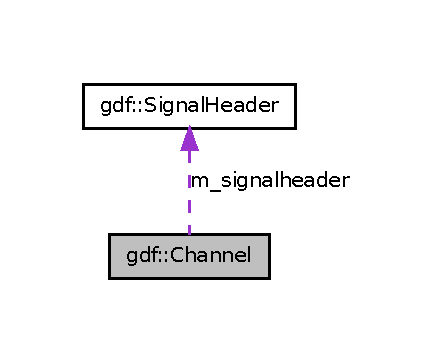
\includegraphics[width=208pt]{classgdf_1_1_channel__coll__graph}
\end{center}
\end{figure}
\subsection*{Public Member Functions}
\begin{DoxyCompactItemize}
\item 
\hypertarget{classgdf_1_1_channel_ac2b2017a6e756749a16af2b9c8509cc0}{
\hyperlink{classgdf_1_1_channel_ac2b2017a6e756749a16af2b9c8509cc0}{Channel} (const \hyperlink{classgdf_1_1_signal_header}{SignalHeader} $\ast$sig\_\-hdr, const size\_\-t length)}
\label{classgdf_1_1_channel_ac2b2017a6e756749a16af2b9c8509cc0}

\begin{DoxyCompactList}\small\item\em Constructor. \item\end{DoxyCompactList}\item 
\hyperlink{classgdf_1_1_channel_af27f9328085d4b662d6039a9fa36b650}{Channel} (const \hyperlink{classgdf_1_1_signal_header}{SignalHeader} $\ast$sig\_\-hdr)
\begin{DoxyCompactList}\small\item\em Constructor. \item\end{DoxyCompactList}\item 
\hypertarget{classgdf_1_1_channel_ac8a48799dbf99cd2d6c93c1de2985d1d}{
virtual \hyperlink{classgdf_1_1_channel_ac8a48799dbf99cd2d6c93c1de2985d1d}{$\sim$Channel} ()}
\label{classgdf_1_1_channel_ac8a48799dbf99cd2d6c93c1de2985d1d}

\begin{DoxyCompactList}\small\item\em Destructor. \item\end{DoxyCompactList}\item 
void \hyperlink{classgdf_1_1_channel_aab748d2a7de10901b179c3ab0088e2bd}{addSamplePhys} (const double value)
\begin{DoxyCompactList}\small\item\em Add a physical sample to the channel. \item\end{DoxyCompactList}\item 
{\footnotesize template$<$typename T $>$ }\\void \hyperlink{classgdf_1_1_channel_af3f1c59ce05c2ce53f67e975475cae0b}{addSampleRaw} (const T rawval)
\begin{DoxyCompactList}\small\item\em Add a raw sample to the channel. \item\end{DoxyCompactList}\item 
void \hyperlink{classgdf_1_1_channel_a9283ade92e758c9b9d069cc2915e2166}{blitSamplesPhys} (const double $\ast$values, size\_\-t num)
\begin{DoxyCompactList}\small\item\em Blit a number of physical samples into channel. \item\end{DoxyCompactList}\item 
{\footnotesize template$<$typename T $>$ }\\void \hyperlink{classgdf_1_1_channel_a4dbee85af31381a4b60807938374d435}{blitSamplesRaw} (const T $\ast$values, size\_\-t num)
\begin{DoxyCompactList}\small\item\em Blit a number of raw samples into channel. \item\end{DoxyCompactList}\item 
void \hyperlink{classgdf_1_1_channel_a076665b0f8cfc07b99cf23bf40aabf46}{fillPhys} (const double value, size\_\-t num)
\begin{DoxyCompactList}\small\item\em Fill a number of samples with the same physical value. \item\end{DoxyCompactList}\item 
{\footnotesize template$<$typename T $>$ }\\void \hyperlink{classgdf_1_1_channel_a8c94145830b7f3de1413a7c79bd791dd}{fillRaw} (const T value, size\_\-t num)
\begin{DoxyCompactList}\small\item\em Fill a number of samples with the same raw value. \item\end{DoxyCompactList}\item 
\hypertarget{classgdf_1_1_channel_a5e11e8837429d02fc4e88c4293e49d19}{
void \hyperlink{classgdf_1_1_channel_a5e11e8837429d02fc4e88c4293e49d19}{setSamplePhys} (size\_\-t pos, double value)}
\label{classgdf_1_1_channel_a5e11e8837429d02fc4e88c4293e49d19}

\begin{DoxyCompactList}\small\item\em set sample value \item\end{DoxyCompactList}\item 
\hypertarget{classgdf_1_1_channel_af332515256e6cc82e8638dc13305c96f}{
double \hyperlink{classgdf_1_1_channel_af332515256e6cc82e8638dc13305c96f}{getSamplePhys} (size\_\-t pos)}
\label{classgdf_1_1_channel_af332515256e6cc82e8638dc13305c96f}

\begin{DoxyCompactList}\small\item\em get sample value \item\end{DoxyCompactList}\item 
void \hyperlink{classgdf_1_1_channel_a12b0aac7591e46cd0bb9bad0d683d1b5}{deblitSamplesPhys} (double $\ast$values, size\_\-t start, size\_\-t num)
\begin{DoxyCompactList}\small\item\em Blit a number of physical samples from channel to buffer. \item\end{DoxyCompactList}\item 
\hypertarget{classgdf_1_1_channel_a280b7c8bddfadc3b8a587b0344750d62}{
{\footnotesize template$<$typename T $>$ }\\void \hyperlink{classgdf_1_1_channel_a280b7c8bddfadc3b8a587b0344750d62}{deblitSamplesRaw} (T $\ast$values, size\_\-t start, size\_\-t num)}
\label{classgdf_1_1_channel_a280b7c8bddfadc3b8a587b0344750d62}

\begin{DoxyCompactList}\small\item\em Blit a number of raw samples from channel to buffer. \item\end{DoxyCompactList}\item 
\hypertarget{classgdf_1_1_channel_a394ca2e97a35c0acc4c9af45e7d7bc3f}{
size\_\-t \hyperlink{classgdf_1_1_channel_a394ca2e97a35c0acc4c9af45e7d7bc3f}{getFree} ()}
\label{classgdf_1_1_channel_a394ca2e97a35c0acc4c9af45e7d7bc3f}

\begin{DoxyCompactList}\small\item\em Get number of free samples. \item\end{DoxyCompactList}\item 
\hypertarget{classgdf_1_1_channel_a103d927127768cc75b61502415b5d892}{
size\_\-t \hyperlink{classgdf_1_1_channel_a103d927127768cc75b61502415b5d892}{getWritten} ()}
\label{classgdf_1_1_channel_a103d927127768cc75b61502415b5d892}

\begin{DoxyCompactList}\small\item\em Get number of written samples. \item\end{DoxyCompactList}\item 
\hypertarget{classgdf_1_1_channel_a2b4461c2601d75de9d8a3a818aacb821}{
uint32 \hyperlink{classgdf_1_1_channel_a2b4461c2601d75de9d8a3a818aacb821}{getTypeID} ()}
\label{classgdf_1_1_channel_a2b4461c2601d75de9d8a3a818aacb821}

\begin{DoxyCompactList}\small\item\em Get type of channel. \item\end{DoxyCompactList}\end{DoxyCompactItemize}
\subsection*{Friends}
\begin{DoxyCompactItemize}
\item 
\hypertarget{classgdf_1_1_channel_a98bbc925b3332bd24bc7964665fa586c}{
std::ostream \& \hyperlink{classgdf_1_1_channel_a98bbc925b3332bd24bc7964665fa586c}{operator$<$$<$} (std::ostream \&out, const \hyperlink{classgdf_1_1_channel}{Channel} \&c)}
\label{classgdf_1_1_channel_a98bbc925b3332bd24bc7964665fa586c}

\begin{DoxyCompactList}\small\item\em \hyperlink{classgdf_1_1_channel}{Channel} Serializer. \item\end{DoxyCompactList}\item 
\hypertarget{classgdf_1_1_channel_ad9bbbcbff8301a7d6fc3ed9636964eb6}{
std::istream \& \hyperlink{classgdf_1_1_channel_ad9bbbcbff8301a7d6fc3ed9636964eb6}{operator$>$$>$} (std::istream \&in, \hyperlink{classgdf_1_1_channel}{Channel} \&c)}
\label{classgdf_1_1_channel_ad9bbbcbff8301a7d6fc3ed9636964eb6}

\begin{DoxyCompactList}\small\item\em \hyperlink{classgdf_1_1_channel}{Channel} Deserializer. \item\end{DoxyCompactList}\end{DoxyCompactItemize}


\subsection{Detailed Description}
Representation of a channel (signal in GDF). 

\subsection{Constructor \& Destructor Documentation}
\hypertarget{classgdf_1_1_channel_af27f9328085d4b662d6039a9fa36b650}{
\index{gdf::Channel@{gdf::Channel}!Channel@{Channel}}
\index{Channel@{Channel}!gdf::Channel@{gdf::Channel}}
\subsubsection[{Channel}]{\setlength{\rightskip}{0pt plus 5cm}gdf::Channel::Channel (
\begin{DoxyParamCaption}
\item[{const {\bf SignalHeader} $\ast$}]{ sig\_\-hdr}
\end{DoxyParamCaption}
)}}
\label{classgdf_1_1_channel_af27f9328085d4b662d6039a9fa36b650}


Constructor. 

\hyperlink{classgdf_1_1_channel}{Channel} length is initialized to channel's samples\_\-per\_\-record. 

\subsection{Member Function Documentation}
\hypertarget{classgdf_1_1_channel_aab748d2a7de10901b179c3ab0088e2bd}{
\index{gdf::Channel@{gdf::Channel}!addSamplePhys@{addSamplePhys}}
\index{addSamplePhys@{addSamplePhys}!gdf::Channel@{gdf::Channel}}
\subsubsection[{addSamplePhys}]{\setlength{\rightskip}{0pt plus 5cm}void gdf::Channel::addSamplePhys (
\begin{DoxyParamCaption}
\item[{const double}]{ value}
\end{DoxyParamCaption}
)}}
\label{classgdf_1_1_channel_aab748d2a7de10901b179c3ab0088e2bd}


Add a physical sample to the channel. 

value is scaled from \mbox{[}phys\_\-min..phys\_\-max\mbox{]} to \mbox{[}dig\_\-min..dig\_\-max\mbox{]} and converted to the channel's data type 

Here is the caller graph for this function:
\nopagebreak
\begin{figure}[H]
\begin{center}
\leavevmode
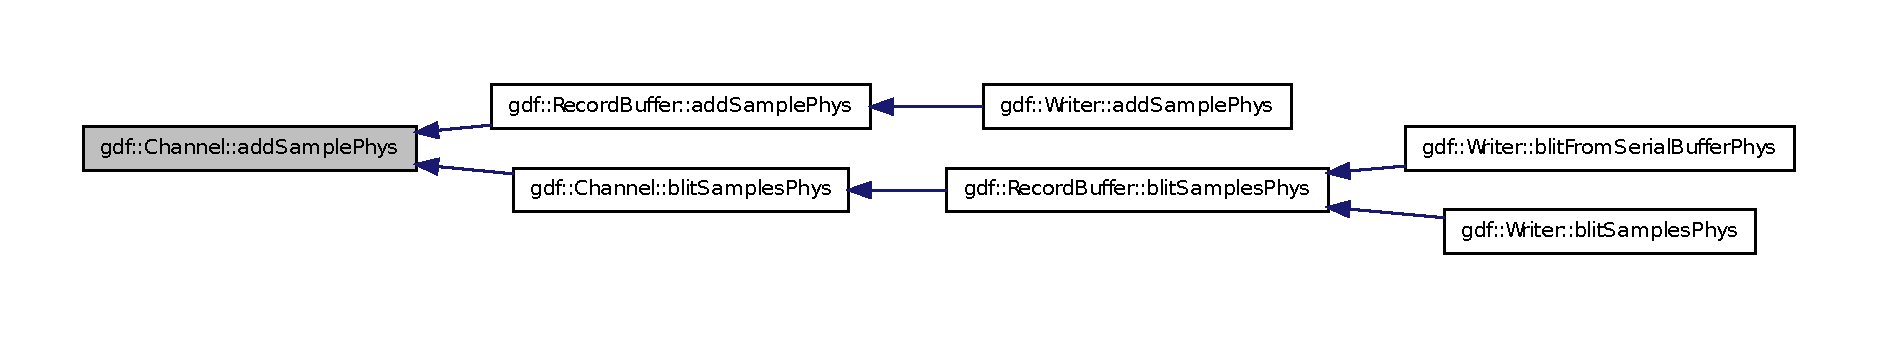
\includegraphics[width=400pt]{classgdf_1_1_channel_aab748d2a7de10901b179c3ab0088e2bd_icgraph}
\end{center}
\end{figure}


\hypertarget{classgdf_1_1_channel_af3f1c59ce05c2ce53f67e975475cae0b}{
\index{gdf::Channel@{gdf::Channel}!addSampleRaw@{addSampleRaw}}
\index{addSampleRaw@{addSampleRaw}!gdf::Channel@{gdf::Channel}}
\subsubsection[{addSampleRaw}]{\setlength{\rightskip}{0pt plus 5cm}template$<$typename T $>$ void gdf::Channel::addSampleRaw (
\begin{DoxyParamCaption}
\item[{const T}]{ rawval}
\end{DoxyParamCaption}
)}}
\label{classgdf_1_1_channel_af3f1c59ce05c2ce53f67e975475cae0b}


Add a raw sample to the channel. 

value is converted to the channel's data type. but otherwise remains unmodified 

Here is the caller graph for this function:
\nopagebreak
\begin{figure}[H]
\begin{center}
\leavevmode
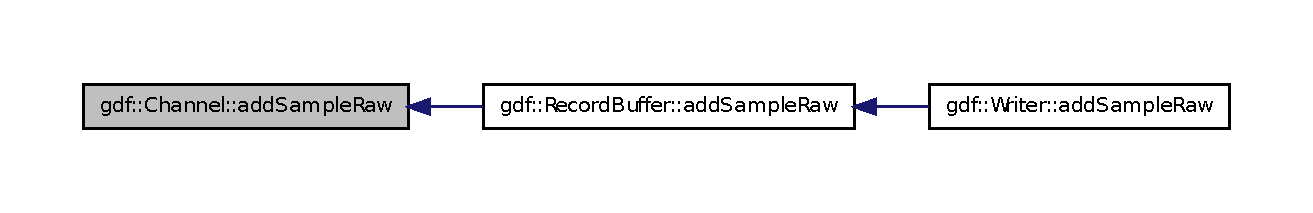
\includegraphics[width=400pt]{classgdf_1_1_channel_af3f1c59ce05c2ce53f67e975475cae0b_icgraph}
\end{center}
\end{figure}


\hypertarget{classgdf_1_1_channel_a9283ade92e758c9b9d069cc2915e2166}{
\index{gdf::Channel@{gdf::Channel}!blitSamplesPhys@{blitSamplesPhys}}
\index{blitSamplesPhys@{blitSamplesPhys}!gdf::Channel@{gdf::Channel}}
\subsubsection[{blitSamplesPhys}]{\setlength{\rightskip}{0pt plus 5cm}void gdf::Channel::blitSamplesPhys (
\begin{DoxyParamCaption}
\item[{const double $\ast$}]{ values, }
\item[{size\_\-t}]{ num}
\end{DoxyParamCaption}
)}}
\label{classgdf_1_1_channel_a9283ade92e758c9b9d069cc2915e2166}


Blit a number of physical samples into channel. 

values are scaled from \mbox{[}phys\_\-min..phys\_\-max\mbox{]} to \mbox{[}dig\_\-min..dig\_\-max\mbox{]} and converted to the channel's data type 

Here is the call graph for this function:
\nopagebreak
\begin{figure}[H]
\begin{center}
\leavevmode
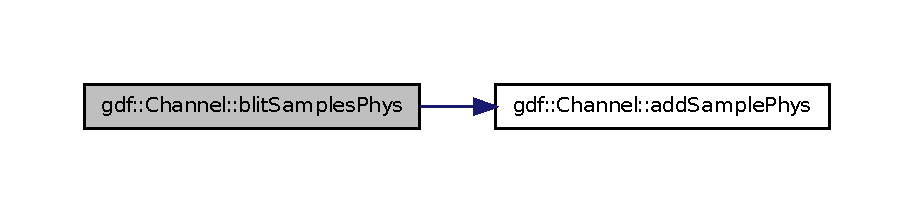
\includegraphics[width=400pt]{classgdf_1_1_channel_a9283ade92e758c9b9d069cc2915e2166_cgraph}
\end{center}
\end{figure}




Here is the caller graph for this function:
\nopagebreak
\begin{figure}[H]
\begin{center}
\leavevmode
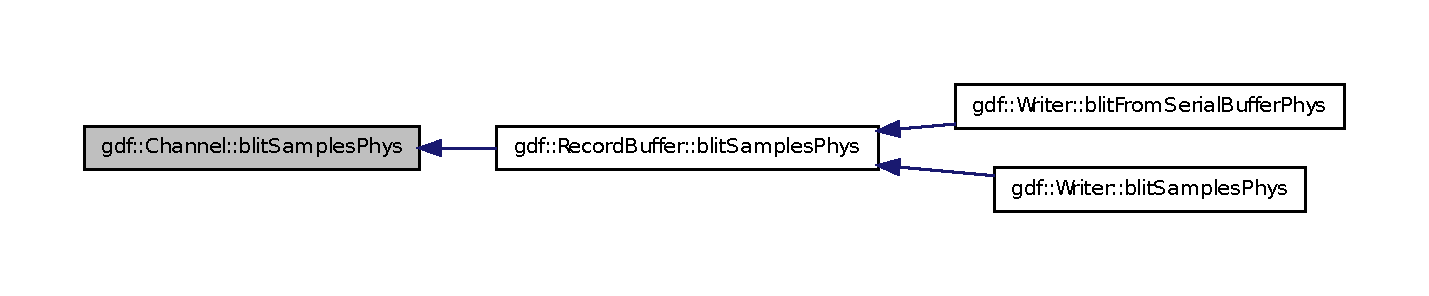
\includegraphics[width=400pt]{classgdf_1_1_channel_a9283ade92e758c9b9d069cc2915e2166_icgraph}
\end{center}
\end{figure}


\hypertarget{classgdf_1_1_channel_a4dbee85af31381a4b60807938374d435}{
\index{gdf::Channel@{gdf::Channel}!blitSamplesRaw@{blitSamplesRaw}}
\index{blitSamplesRaw@{blitSamplesRaw}!gdf::Channel@{gdf::Channel}}
\subsubsection[{blitSamplesRaw}]{\setlength{\rightskip}{0pt plus 5cm}template$<$typename T $>$ void gdf::Channel::blitSamplesRaw (
\begin{DoxyParamCaption}
\item[{const T $\ast$}]{ values, }
\item[{size\_\-t}]{ num}
\end{DoxyParamCaption}
)}}
\label{classgdf_1_1_channel_a4dbee85af31381a4b60807938374d435}


Blit a number of raw samples into channel. 

values are converted to the channel's data type but otherwise remains unmodified 

Here is the caller graph for this function:
\nopagebreak
\begin{figure}[H]
\begin{center}
\leavevmode
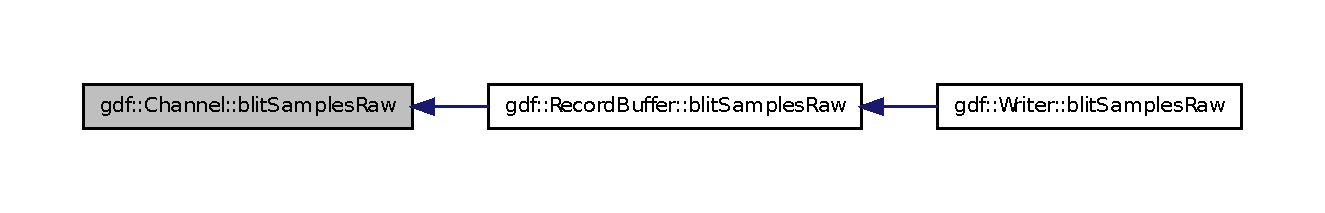
\includegraphics[width=400pt]{classgdf_1_1_channel_a4dbee85af31381a4b60807938374d435_icgraph}
\end{center}
\end{figure}


\hypertarget{classgdf_1_1_channel_a12b0aac7591e46cd0bb9bad0d683d1b5}{
\index{gdf::Channel@{gdf::Channel}!deblitSamplesPhys@{deblitSamplesPhys}}
\index{deblitSamplesPhys@{deblitSamplesPhys}!gdf::Channel@{gdf::Channel}}
\subsubsection[{deblitSamplesPhys}]{\setlength{\rightskip}{0pt plus 5cm}void gdf::Channel::deblitSamplesPhys (
\begin{DoxyParamCaption}
\item[{double $\ast$}]{ values, }
\item[{size\_\-t}]{ start, }
\item[{size\_\-t}]{ num}
\end{DoxyParamCaption}
)}}
\label{classgdf_1_1_channel_a12b0aac7591e46cd0bb9bad0d683d1b5}


Blit a number of physical samples from channel to buffer. 

values are scaled from \mbox{[}dig\_\-min..dig\_\-max\mbox{]} to \mbox{[}phys\_\-min..phys\_\-max\mbox{]} and converted to double 

Here is the call graph for this function:
\nopagebreak
\begin{figure}[H]
\begin{center}
\leavevmode
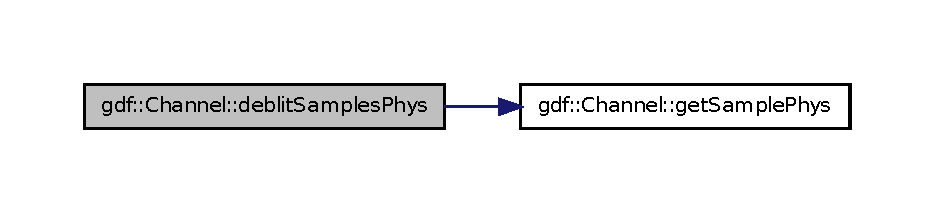
\includegraphics[width=400pt]{classgdf_1_1_channel_a12b0aac7591e46cd0bb9bad0d683d1b5_cgraph}
\end{center}
\end{figure}




Here is the caller graph for this function:
\nopagebreak
\begin{figure}[H]
\begin{center}
\leavevmode
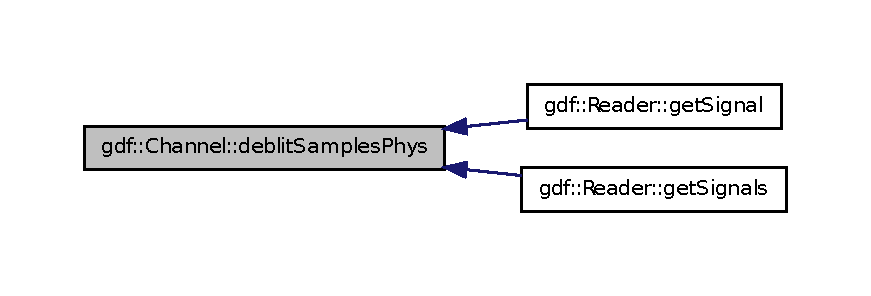
\includegraphics[width=400pt]{classgdf_1_1_channel_a12b0aac7591e46cd0bb9bad0d683d1b5_icgraph}
\end{center}
\end{figure}


\hypertarget{classgdf_1_1_channel_a076665b0f8cfc07b99cf23bf40aabf46}{
\index{gdf::Channel@{gdf::Channel}!fillPhys@{fillPhys}}
\index{fillPhys@{fillPhys}!gdf::Channel@{gdf::Channel}}
\subsubsection[{fillPhys}]{\setlength{\rightskip}{0pt plus 5cm}void gdf::Channel::fillPhys (
\begin{DoxyParamCaption}
\item[{const double}]{ value, }
\item[{size\_\-t}]{ num}
\end{DoxyParamCaption}
)}}
\label{classgdf_1_1_channel_a076665b0f8cfc07b99cf23bf40aabf46}


Fill a number of samples with the same physical value. 

value is scaled from \mbox{[}phys\_\-min..phys\_\-max\mbox{]} to \mbox{[}dig\_\-min..dig\_\-max\mbox{]} and converted to the channel's data type \hypertarget{classgdf_1_1_channel_a8c94145830b7f3de1413a7c79bd791dd}{
\index{gdf::Channel@{gdf::Channel}!fillRaw@{fillRaw}}
\index{fillRaw@{fillRaw}!gdf::Channel@{gdf::Channel}}
\subsubsection[{fillRaw}]{\setlength{\rightskip}{0pt plus 5cm}template$<$typename T $>$ void gdf::Channel::fillRaw (
\begin{DoxyParamCaption}
\item[{const T}]{ value, }
\item[{size\_\-t}]{ num}
\end{DoxyParamCaption}
)}}
\label{classgdf_1_1_channel_a8c94145830b7f3de1413a7c79bd791dd}


Fill a number of samples with the same raw value. 

value is converted to the channel's data type but otherwise remains unmodified 

The documentation for this class was generated from the following files:\begin{DoxyCompactItemize}
\item 
include/GDF/Channel.h\item 
src/Channel.cpp\end{DoxyCompactItemize}

\hypertarget{classgdf_1_1_channel_data}{
\section{gdf::ChannelData$<$ T $>$ Class Template Reference}
\label{classgdf_1_1_channel_data}\index{gdf::ChannelData@{gdf::ChannelData}}
}


Contains data samples for a channel of given type and length.  




{\ttfamily \#include $<$ChannelData.h$>$}



Inherits \hyperlink{classgdf_1_1_channel_data_base}{gdf::ChannelDataBase}.



Collaboration diagram for gdf::ChannelData$<$ T $>$:
\nopagebreak
\begin{figure}[H]
\begin{center}
\leavevmode
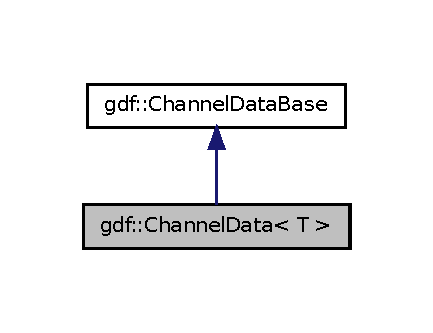
\includegraphics[width=208pt]{classgdf_1_1_channel_data__coll__graph}
\end{center}
\end{figure}
\subsection*{Public Member Functions}
\begin{DoxyCompactItemize}
\item 
\hypertarget{classgdf_1_1_channel_data_a493aade9101eb8d60a5783c3b37b04fc}{
\hyperlink{classgdf_1_1_channel_data_a493aade9101eb8d60a5783c3b37b04fc}{ChannelData} (size\_\-t length)}
\label{classgdf_1_1_channel_data_a493aade9101eb8d60a5783c3b37b04fc}

\begin{DoxyCompactList}\small\item\em Constructor. \item\end{DoxyCompactList}\item 
\hypertarget{classgdf_1_1_channel_data_a43a64284e5eb513e988514fae70474d6}{
virtual \hyperlink{classgdf_1_1_channel_data_a43a64284e5eb513e988514fae70474d6}{$\sim$ChannelData} ()}
\label{classgdf_1_1_channel_data_a43a64284e5eb513e988514fae70474d6}

\begin{DoxyCompactList}\small\item\em Destructor. \item\end{DoxyCompactList}\item 
\hypertarget{classgdf_1_1_channel_data_a72660b2608d86888a61a51efad28007c}{
void \hyperlink{classgdf_1_1_channel_data_a72660b2608d86888a61a51efad28007c}{addSample} (const T value)}
\label{classgdf_1_1_channel_data_a72660b2608d86888a61a51efad28007c}

\begin{DoxyCompactList}\small\item\em Add a single sample to the channel. \hyperlink{classgdf_1_1_channel}{Channel} must not be full. \item\end{DoxyCompactList}\item 
\hypertarget{classgdf_1_1_channel_data_a5055b2f003e69afd238b064e795adc53}{
void \hyperlink{classgdf_1_1_channel_data_a5055b2f003e69afd238b064e795adc53}{blitSamples} (const T $\ast$values, const size\_\-t num)}
\label{classgdf_1_1_channel_data_a5055b2f003e69afd238b064e795adc53}

\begin{DoxyCompactList}\small\item\em Blit a given number of samples into channel. That number of samples must be free. \item\end{DoxyCompactList}\item 
\hypertarget{classgdf_1_1_channel_data_afebe6672e849f3ca33804e8fb5e73d8c}{
void \hyperlink{classgdf_1_1_channel_data_afebe6672e849f3ca33804e8fb5e73d8c}{fill} (const T value, const size\_\-t num)}
\label{classgdf_1_1_channel_data_afebe6672e849f3ca33804e8fb5e73d8c}

\begin{DoxyCompactList}\small\item\em Fills a given number of samples with value. That number of samples must be free. \item\end{DoxyCompactList}\item 
\hypertarget{classgdf_1_1_channel_data_a5f7d5b6e536b749b5d6e6d0ec845d43d}{
void \hyperlink{classgdf_1_1_channel_data_a5f7d5b6e536b749b5d6e6d0ec845d43d}{setSample} (size\_\-t pos, T rawval)}
\label{classgdf_1_1_channel_data_a5f7d5b6e536b749b5d6e6d0ec845d43d}

\begin{DoxyCompactList}\small\item\em set sapmle value \item\end{DoxyCompactList}\item 
\hypertarget{classgdf_1_1_channel_data_a92c2adf653075fc97b7230981c1dd62f}{
T \hyperlink{classgdf_1_1_channel_data_a92c2adf653075fc97b7230981c1dd62f}{getSample} (size\_\-t pos, T)}
\label{classgdf_1_1_channel_data_a92c2adf653075fc97b7230981c1dd62f}

\begin{DoxyCompactList}\small\item\em get sapmle value \item\end{DoxyCompactList}\item 
\hypertarget{classgdf_1_1_channel_data_a2d1e7afb4eb90587dfe6a8b309fae185}{
size\_\-t \hyperlink{classgdf_1_1_channel_data_a2d1e7afb4eb90587dfe6a8b309fae185}{getFree} ()}
\label{classgdf_1_1_channel_data_a2d1e7afb4eb90587dfe6a8b309fae185}

\begin{DoxyCompactList}\small\item\em Get number of free samples. \item\end{DoxyCompactList}\item 
\hypertarget{classgdf_1_1_channel_data_a140a1309e5b054b104ea2f18bd42b01a}{
virtual size\_\-t \hyperlink{classgdf_1_1_channel_data_a140a1309e5b054b104ea2f18bd42b01a}{getWritten} ()}
\label{classgdf_1_1_channel_data_a140a1309e5b054b104ea2f18bd42b01a}

\begin{DoxyCompactList}\small\item\em Get number of written samples. \item\end{DoxyCompactList}\item 
\hypertarget{classgdf_1_1_channel_data_a873a796235e69086ae360998d24e159d}{
void \hyperlink{classgdf_1_1_channel_data_a873a796235e69086ae360998d24e159d}{tostream} (std::ostream \&out)}
\label{classgdf_1_1_channel_data_a873a796235e69086ae360998d24e159d}

\begin{DoxyCompactList}\small\item\em Serializer. \item\end{DoxyCompactList}\item 
\hypertarget{classgdf_1_1_channel_data_a5ec0367f1377269cdeba97de05e1280f}{
void \hyperlink{classgdf_1_1_channel_data_a5ec0367f1377269cdeba97de05e1280f}{fromstream} (std::istream \&in)}
\label{classgdf_1_1_channel_data_a5ec0367f1377269cdeba97de05e1280f}

\begin{DoxyCompactList}\small\item\em Deserializer. \item\end{DoxyCompactList}\end{DoxyCompactItemize}
\subsection*{Protected Member Functions}
\begin{DoxyCompactItemize}
\item 
\hypertarget{classgdf_1_1_channel_data_ad17629e054633b2a414bf66e436b4880}{
std::vector$<$ T $>$ \& \hyperlink{classgdf_1_1_channel_data_ad17629e054633b2a414bf66e436b4880}{getData} ()}
\label{classgdf_1_1_channel_data_ad17629e054633b2a414bf66e436b4880}

\begin{DoxyCompactList}\small\item\em Get reference to data. \item\end{DoxyCompactList}\item 
\hypertarget{classgdf_1_1_channel_data_abc52094c23daca566e177d4a6b6e1e23}{
std::vector$<$ T $>$ $\ast$ \hyperlink{classgdf_1_1_channel_data_abc52094c23daca566e177d4a6b6e1e23}{getDataPtr} ()}
\label{classgdf_1_1_channel_data_abc52094c23daca566e177d4a6b6e1e23}

\begin{DoxyCompactList}\small\item\em Get pointer to data. \item\end{DoxyCompactList}\end{DoxyCompactItemize}


\subsection{Detailed Description}
\subsubsection*{template$<$typename T$>$ class gdf::ChannelData$<$ T $>$}

Contains data samples for a channel of given type and length. Only access functions of type T are reimplemented from \hyperlink{classgdf_1_1_channel_data_base}{ChannelDataBase}. Calling \hyperlink{classgdf_1_1_channel_data_a72660b2608d86888a61a51efad28007c}{addSample()}, \hyperlink{classgdf_1_1_channel_data_a5055b2f003e69afd238b064e795adc53}{blitSamples()} or \hyperlink{classgdf_1_1_channel_data_afebe6672e849f3ca33804e8fb5e73d8c}{fill()} with the wrong data type throws an exception. 

The documentation for this class was generated from the following file:\begin{DoxyCompactItemize}
\item 
include/GDF/ChannelData.h\end{DoxyCompactItemize}

\hypertarget{classgdf_1_1_channel_data_base}{
\section{gdf::ChannelDataBase Class Reference}
\label{classgdf_1_1_channel_data_base}\index{gdf::ChannelDataBase@{gdf::ChannelDataBase}}
}


Base class that provides access to channels of different types.  




{\ttfamily \#include $<$ChannelDataBase.h$>$}



Inherited by \hyperlink{classgdf_1_1_channel_data}{gdf::ChannelData$<$ T $>$}.

\subsection*{Public Member Functions}
\begin{DoxyCompactItemize}
\item 
\hypertarget{classgdf_1_1_channel_data_base_addc4f27c1d0edecf3f641cab0c03e7a7}{
virtual void {\bfseries addSample} (const int8)}
\label{classgdf_1_1_channel_data_base_addc4f27c1d0edecf3f641cab0c03e7a7}

\item 
\hypertarget{classgdf_1_1_channel_data_base_addd8e902bc4f87ba595083a793c2d5df}{
virtual void {\bfseries addSample} (const uint8)}
\label{classgdf_1_1_channel_data_base_addd8e902bc4f87ba595083a793c2d5df}

\item 
\hypertarget{classgdf_1_1_channel_data_base_a7105fca54334e4ef91d209e04a1eea96}{
virtual void {\bfseries addSample} (const int16)}
\label{classgdf_1_1_channel_data_base_a7105fca54334e4ef91d209e04a1eea96}

\item 
\hypertarget{classgdf_1_1_channel_data_base_a6fe3f6d20c2b89a16d87347f45f5fef8}{
virtual void {\bfseries addSample} (const uint16)}
\label{classgdf_1_1_channel_data_base_a6fe3f6d20c2b89a16d87347f45f5fef8}

\item 
\hypertarget{classgdf_1_1_channel_data_base_a3d69464c498d784d53283c377d1dadd4}{
virtual void {\bfseries addSample} (const int32)}
\label{classgdf_1_1_channel_data_base_a3d69464c498d784d53283c377d1dadd4}

\item 
\hypertarget{classgdf_1_1_channel_data_base_afd472b9b39d8fbe78e2a4e028ff8affa}{
virtual void {\bfseries addSample} (const uint32)}
\label{classgdf_1_1_channel_data_base_afd472b9b39d8fbe78e2a4e028ff8affa}

\item 
\hypertarget{classgdf_1_1_channel_data_base_afc25653362a4bb65785eb6473aff6736}{
virtual void {\bfseries addSample} (const int64)}
\label{classgdf_1_1_channel_data_base_afc25653362a4bb65785eb6473aff6736}

\item 
\hypertarget{classgdf_1_1_channel_data_base_ae3b7c456d2e329259ddde009da767876}{
virtual void {\bfseries addSample} (const uint64)}
\label{classgdf_1_1_channel_data_base_ae3b7c456d2e329259ddde009da767876}

\item 
\hypertarget{classgdf_1_1_channel_data_base_a9d9ff56c2b381c51214fab981421707f}{
virtual void {\bfseries addSample} (const float32)}
\label{classgdf_1_1_channel_data_base_a9d9ff56c2b381c51214fab981421707f}

\item 
\hypertarget{classgdf_1_1_channel_data_base_a2dadb66b6846081b1342d75c6d9e6c43}{
virtual void {\bfseries addSample} (const float64)}
\label{classgdf_1_1_channel_data_base_a2dadb66b6846081b1342d75c6d9e6c43}

\item 
\hypertarget{classgdf_1_1_channel_data_base_ad1df5140285f394dafa0d9022487ff97}{
virtual void {\bfseries blitSamples} (const int8 $\ast$, const size\_\-t)}
\label{classgdf_1_1_channel_data_base_ad1df5140285f394dafa0d9022487ff97}

\item 
\hypertarget{classgdf_1_1_channel_data_base_a127a06c8b2f3ac3766ea350568a0476e}{
virtual void {\bfseries blitSamples} (const uint8 $\ast$, const size\_\-t)}
\label{classgdf_1_1_channel_data_base_a127a06c8b2f3ac3766ea350568a0476e}

\item 
\hypertarget{classgdf_1_1_channel_data_base_a75bbf3497641eec5f82998f9a32ffa6d}{
virtual void {\bfseries blitSamples} (const int16 $\ast$, const size\_\-t)}
\label{classgdf_1_1_channel_data_base_a75bbf3497641eec5f82998f9a32ffa6d}

\item 
\hypertarget{classgdf_1_1_channel_data_base_a3ed5f4fba584aa6087d2f786e69ed48b}{
virtual void {\bfseries blitSamples} (const uint16 $\ast$, const size\_\-t)}
\label{classgdf_1_1_channel_data_base_a3ed5f4fba584aa6087d2f786e69ed48b}

\item 
\hypertarget{classgdf_1_1_channel_data_base_a2a47013787265df595c9cfe44ab03eda}{
virtual void {\bfseries blitSamples} (const int32 $\ast$, const size\_\-t)}
\label{classgdf_1_1_channel_data_base_a2a47013787265df595c9cfe44ab03eda}

\item 
\hypertarget{classgdf_1_1_channel_data_base_a6d7edf2dcbf3b4e91581e5038f38bb7a}{
virtual void {\bfseries blitSamples} (const uint32 $\ast$, const size\_\-t)}
\label{classgdf_1_1_channel_data_base_a6d7edf2dcbf3b4e91581e5038f38bb7a}

\item 
\hypertarget{classgdf_1_1_channel_data_base_a74c299f35ae398da856cc037c2d6d4bf}{
virtual void {\bfseries blitSamples} (const int64 $\ast$, const size\_\-t)}
\label{classgdf_1_1_channel_data_base_a74c299f35ae398da856cc037c2d6d4bf}

\item 
\hypertarget{classgdf_1_1_channel_data_base_a32c1625fe7e54739aec0e6682d77a833}{
virtual void {\bfseries blitSamples} (const uint64 $\ast$, const size\_\-t)}
\label{classgdf_1_1_channel_data_base_a32c1625fe7e54739aec0e6682d77a833}

\item 
\hypertarget{classgdf_1_1_channel_data_base_a4a8ae538a6e045dbd94a8a1487360a1f}{
virtual void {\bfseries blitSamples} (const float32 $\ast$, const size\_\-t)}
\label{classgdf_1_1_channel_data_base_a4a8ae538a6e045dbd94a8a1487360a1f}

\item 
\hypertarget{classgdf_1_1_channel_data_base_aa83b8a40a8e1055cda47fef0a55156b7}{
virtual void {\bfseries blitSamples} (const float64 $\ast$, const size\_\-t)}
\label{classgdf_1_1_channel_data_base_aa83b8a40a8e1055cda47fef0a55156b7}

\item 
\hypertarget{classgdf_1_1_channel_data_base_aad66caf102091d0b203f6245c39b960c}{
virtual void {\bfseries fill} (const int8, const size\_\-t)}
\label{classgdf_1_1_channel_data_base_aad66caf102091d0b203f6245c39b960c}

\item 
\hypertarget{classgdf_1_1_channel_data_base_aced7b48ea4079c8e9d50161e99114a46}{
virtual void {\bfseries fill} (const uint8, const size\_\-t)}
\label{classgdf_1_1_channel_data_base_aced7b48ea4079c8e9d50161e99114a46}

\item 
\hypertarget{classgdf_1_1_channel_data_base_af53bdd2dafcdc13d5394f7861dc77181}{
virtual void {\bfseries fill} (const int16, const size\_\-t)}
\label{classgdf_1_1_channel_data_base_af53bdd2dafcdc13d5394f7861dc77181}

\item 
\hypertarget{classgdf_1_1_channel_data_base_aaa262c6fdb92f5beb3804031f6f25b7f}{
virtual void {\bfseries fill} (const uint16, const size\_\-t)}
\label{classgdf_1_1_channel_data_base_aaa262c6fdb92f5beb3804031f6f25b7f}

\item 
\hypertarget{classgdf_1_1_channel_data_base_a121ce49a2f1e1e64bcd3b41869fb5fa3}{
virtual void {\bfseries fill} (const int32, const size\_\-t)}
\label{classgdf_1_1_channel_data_base_a121ce49a2f1e1e64bcd3b41869fb5fa3}

\item 
\hypertarget{classgdf_1_1_channel_data_base_ac7b5abe94d7d068eeb96cad924335889}{
virtual void {\bfseries fill} (const uint32, const size\_\-t)}
\label{classgdf_1_1_channel_data_base_ac7b5abe94d7d068eeb96cad924335889}

\item 
\hypertarget{classgdf_1_1_channel_data_base_a3a67a754117caa411204cbe821e74284}{
virtual void {\bfseries fill} (const int64, const size\_\-t)}
\label{classgdf_1_1_channel_data_base_a3a67a754117caa411204cbe821e74284}

\item 
\hypertarget{classgdf_1_1_channel_data_base_a517a62fdcfe0b0491b7bc1c736ec017e}{
virtual void {\bfseries fill} (const uint64, const size\_\-t)}
\label{classgdf_1_1_channel_data_base_a517a62fdcfe0b0491b7bc1c736ec017e}

\item 
\hypertarget{classgdf_1_1_channel_data_base_a1970d44bfb982519a7b3a25835c80efe}{
virtual void {\bfseries fill} (const float32, const size\_\-t)}
\label{classgdf_1_1_channel_data_base_a1970d44bfb982519a7b3a25835c80efe}

\item 
\hypertarget{classgdf_1_1_channel_data_base_a752ca98ba08fec2021cd16fbf0ea1bb6}{
virtual void {\bfseries fill} (const float64, const size\_\-t)}
\label{classgdf_1_1_channel_data_base_a752ca98ba08fec2021cd16fbf0ea1bb6}

\item 
\hypertarget{classgdf_1_1_channel_data_base_a404d958b7b5f4ff80da471d373775b65}{
virtual void {\bfseries setSample} (size\_\-t, int8)}
\label{classgdf_1_1_channel_data_base_a404d958b7b5f4ff80da471d373775b65}

\item 
\hypertarget{classgdf_1_1_channel_data_base_a6193247362943cb78fbe74fe3f11b2d4}{
virtual void {\bfseries setSample} (size\_\-t, uint8)}
\label{classgdf_1_1_channel_data_base_a6193247362943cb78fbe74fe3f11b2d4}

\item 
\hypertarget{classgdf_1_1_channel_data_base_a578e8e03f7146ae4ee151e0d3e10e811}{
virtual void {\bfseries setSample} (size\_\-t, int16)}
\label{classgdf_1_1_channel_data_base_a578e8e03f7146ae4ee151e0d3e10e811}

\item 
\hypertarget{classgdf_1_1_channel_data_base_ac5ca0df901cff713e9ab430bff8b79e6}{
virtual void {\bfseries setSample} (size\_\-t, uint16)}
\label{classgdf_1_1_channel_data_base_ac5ca0df901cff713e9ab430bff8b79e6}

\item 
\hypertarget{classgdf_1_1_channel_data_base_a28832ba1a26c18b19b5f545b8bf79769}{
virtual void {\bfseries setSample} (size\_\-t, int32)}
\label{classgdf_1_1_channel_data_base_a28832ba1a26c18b19b5f545b8bf79769}

\item 
\hypertarget{classgdf_1_1_channel_data_base_a20943158b1801b33c0fc2f2d70e0c184}{
virtual void {\bfseries setSample} (size\_\-t, uint32)}
\label{classgdf_1_1_channel_data_base_a20943158b1801b33c0fc2f2d70e0c184}

\item 
\hypertarget{classgdf_1_1_channel_data_base_a2f80be47b2cfbb99eef50c91bdea64bf}{
virtual void {\bfseries setSample} (size\_\-t, int64)}
\label{classgdf_1_1_channel_data_base_a2f80be47b2cfbb99eef50c91bdea64bf}

\item 
\hypertarget{classgdf_1_1_channel_data_base_a3f9d148ca2ae0c7b97de02aa4e9062ad}{
virtual void {\bfseries setSample} (size\_\-t, uint64)}
\label{classgdf_1_1_channel_data_base_a3f9d148ca2ae0c7b97de02aa4e9062ad}

\item 
\hypertarget{classgdf_1_1_channel_data_base_a0662cf679913f8469e51b2b9bf3538c3}{
virtual void {\bfseries setSample} (size\_\-t, float32)}
\label{classgdf_1_1_channel_data_base_a0662cf679913f8469e51b2b9bf3538c3}

\item 
\hypertarget{classgdf_1_1_channel_data_base_ae927893f6cb10dc9f7fe0f78bd9f2d51}{
virtual void {\bfseries setSample} (size\_\-t, float64)}
\label{classgdf_1_1_channel_data_base_ae927893f6cb10dc9f7fe0f78bd9f2d51}

\item 
\hypertarget{classgdf_1_1_channel_data_base_a95ff1b51ace922e5a2e86d399ed51f96}{
virtual int8 {\bfseries getSample} (size\_\-t, int8)}
\label{classgdf_1_1_channel_data_base_a95ff1b51ace922e5a2e86d399ed51f96}

\item 
\hypertarget{classgdf_1_1_channel_data_base_a4019971fb272a9e8691da8ff50c75297}{
virtual uint8 {\bfseries getSample} (size\_\-t, uint8)}
\label{classgdf_1_1_channel_data_base_a4019971fb272a9e8691da8ff50c75297}

\item 
\hypertarget{classgdf_1_1_channel_data_base_aa5fb6989e150b610067e7680cfe33fdd}{
virtual int16 {\bfseries getSample} (size\_\-t, int16)}
\label{classgdf_1_1_channel_data_base_aa5fb6989e150b610067e7680cfe33fdd}

\item 
\hypertarget{classgdf_1_1_channel_data_base_a70254b0f5236eb5565fe4fe68d8c6245}{
virtual uint16 {\bfseries getSample} (size\_\-t, uint16)}
\label{classgdf_1_1_channel_data_base_a70254b0f5236eb5565fe4fe68d8c6245}

\item 
\hypertarget{classgdf_1_1_channel_data_base_a17e587bbca723eb56a45f6ce114287f1}{
virtual int32 {\bfseries getSample} (size\_\-t, int32)}
\label{classgdf_1_1_channel_data_base_a17e587bbca723eb56a45f6ce114287f1}

\item 
\hypertarget{classgdf_1_1_channel_data_base_a07fac79a28d18ce86d7d2c61ef72a22e}{
virtual uint32 {\bfseries getSample} (size\_\-t, uint32)}
\label{classgdf_1_1_channel_data_base_a07fac79a28d18ce86d7d2c61ef72a22e}

\item 
\hypertarget{classgdf_1_1_channel_data_base_ae2a01a68732f491ea78da1e6f764e896}{
virtual int64 {\bfseries getSample} (size\_\-t, int64)}
\label{classgdf_1_1_channel_data_base_ae2a01a68732f491ea78da1e6f764e896}

\item 
\hypertarget{classgdf_1_1_channel_data_base_a357d17b095e0bc85561a351661000d8c}{
virtual uint64 {\bfseries getSample} (size\_\-t, uint64)}
\label{classgdf_1_1_channel_data_base_a357d17b095e0bc85561a351661000d8c}

\item 
\hypertarget{classgdf_1_1_channel_data_base_a332d0dddf57f808d2312488d951f7948}{
virtual float32 {\bfseries getSample} (size\_\-t, float32)}
\label{classgdf_1_1_channel_data_base_a332d0dddf57f808d2312488d951f7948}

\item 
\hypertarget{classgdf_1_1_channel_data_base_a42a0f320e1b541a0c1e7c64ffc134853}{
virtual float64 {\bfseries getSample} (size\_\-t, float64)}
\label{classgdf_1_1_channel_data_base_a42a0f320e1b541a0c1e7c64ffc134853}

\item 
\hypertarget{classgdf_1_1_channel_data_base_a28590d9eaba4765db13be9b9d2634f49}{
virtual size\_\-t \hyperlink{classgdf_1_1_channel_data_base_a28590d9eaba4765db13be9b9d2634f49}{getFree} ()=0}
\label{classgdf_1_1_channel_data_base_a28590d9eaba4765db13be9b9d2634f49}

\begin{DoxyCompactList}\small\item\em Get number of free samples. \item\end{DoxyCompactList}\item 
\hypertarget{classgdf_1_1_channel_data_base_afeb7e95c279315fd7c94cd2be56fe652}{
virtual size\_\-t \hyperlink{classgdf_1_1_channel_data_base_afeb7e95c279315fd7c94cd2be56fe652}{getWritten} ()=0}
\label{classgdf_1_1_channel_data_base_afeb7e95c279315fd7c94cd2be56fe652}

\begin{DoxyCompactList}\small\item\em Get number of written samples. \item\end{DoxyCompactList}\item 
\hypertarget{classgdf_1_1_channel_data_base_adb5aada219a951e591d6a41d3eaf2594}{
virtual void \hyperlink{classgdf_1_1_channel_data_base_adb5aada219a951e591d6a41d3eaf2594}{tostream} (std::ostream \&out)=0}
\label{classgdf_1_1_channel_data_base_adb5aada219a951e591d6a41d3eaf2594}

\begin{DoxyCompactList}\small\item\em Serializer. \item\end{DoxyCompactList}\item 
\hypertarget{classgdf_1_1_channel_data_base_a47cd719f239610c4676296a5889e1878}{
virtual void \hyperlink{classgdf_1_1_channel_data_base_a47cd719f239610c4676296a5889e1878}{fromstream} (std::istream \&in)=0}
\label{classgdf_1_1_channel_data_base_a47cd719f239610c4676296a5889e1878}

\begin{DoxyCompactList}\small\item\em Deserializer. \item\end{DoxyCompactList}\end{DoxyCompactItemize}


\subsection{Detailed Description}
Base class that provides access to channels of different types. Meant only for internal use. This class provides overloaded access functions for each data type supported in gdf. The actual implementation of \hyperlink{classgdf_1_1_channel_data}{ChannelData} must reimplement access functions for it's data type. 

The documentation for this class was generated from the following file:\begin{DoxyCompactItemize}
\item 
include/GDF/ChannelDataBase.h\end{DoxyCompactItemize}

\hypertarget{classgdf_1_1exception_1_1corrupt__recordbuffer}{
\section{gdf::exception::corrupt\_\-recordbuffer Class Reference}
\label{classgdf_1_1exception_1_1corrupt__recordbuffer}\index{gdf::exception::corrupt\_\-recordbuffer@{gdf::exception::corrupt\_\-recordbuffer}}
}


\hyperlink{classgdf_1_1_record}{Record} Buffer is corrupt. This likely indicates an internal programming error.  




{\ttfamily \#include $<$Exceptions.h$>$}

\subsection*{Public Member Functions}
\begin{DoxyCompactItemize}
\item 
\hypertarget{classgdf_1_1exception_1_1corrupt__recordbuffer_ad2f1cee8739858a2990d9bf0bb1e971f}{
{\bfseries corrupt\_\-recordbuffer} (std::string str)}
\label{classgdf_1_1exception_1_1corrupt__recordbuffer_ad2f1cee8739858a2990d9bf0bb1e971f}

\end{DoxyCompactItemize}


\subsection{Detailed Description}
\hyperlink{classgdf_1_1_record}{Record} Buffer is corrupt. This likely indicates an internal programming error. 

The documentation for this class was generated from the following file:\begin{DoxyCompactItemize}
\item 
include/GDF/Exceptions.h\end{DoxyCompactItemize}

\hypertarget{classgdf_1_1exception_1_1empty__container}{
\section{gdf::exception::empty\_\-container Class Reference}
\label{classgdf_1_1exception_1_1empty__container}\index{gdf::exception::empty\_\-container@{gdf::exception::empty\_\-container}}
}


A container of some sort (list, vector, array, ... ) is empty.  




{\ttfamily \#include $<$Exceptions.h$>$}

\subsection*{Public Member Functions}
\begin{DoxyCompactItemize}
\item 
\hypertarget{classgdf_1_1exception_1_1empty__container_a226e3ca46a0a3c658896d956bffb1a0a}{
{\bfseries empty\_\-container} (std::string str)}
\label{classgdf_1_1exception_1_1empty__container_a226e3ca46a0a3c658896d956bffb1a0a}

\end{DoxyCompactItemize}


\subsection{Detailed Description}
A container of some sort (list, vector, array, ... ) is empty. 

The documentation for this class was generated from the following file:\begin{DoxyCompactItemize}
\item 
include/GDF/Exceptions.h\end{DoxyCompactItemize}

\hypertarget{classgdf_1_1_event_header}{
\section{gdf::EventHeader Class Reference}
\label{classgdf_1_1_event_header}\index{gdf::EventHeader@{gdf::EventHeader}}
}


Class that provides access to GDF events.  




{\ttfamily \#include $<$EventHeader.h$>$}

\subsection*{Public Member Functions}
\begin{DoxyCompactItemize}
\item 
\hypertarget{classgdf_1_1_event_header_a2182bca6b8218be97f069e74c27ad81c}{
\hyperlink{classgdf_1_1_event_header_a2182bca6b8218be97f069e74c27ad81c}{EventHeader} ()}
\label{classgdf_1_1_event_header_a2182bca6b8218be97f069e74c27ad81c}

\begin{DoxyCompactList}\small\item\em Constructor. \item\end{DoxyCompactList}\item 
\hypertarget{classgdf_1_1_event_header_a20252e9799545069a2ec27f78b137c11}{
virtual \hyperlink{classgdf_1_1_event_header_a20252e9799545069a2ec27f78b137c11}{$\sim$EventHeader} ()}
\label{classgdf_1_1_event_header_a20252e9799545069a2ec27f78b137c11}

\begin{DoxyCompactList}\small\item\em Destructor. \item\end{DoxyCompactList}\item 
\hypertarget{classgdf_1_1_event_header_ac77886ed06b41e7a2ac6ba8811c68de1}{
void \hyperlink{classgdf_1_1_event_header_ac77886ed06b41e7a2ac6ba8811c68de1}{toStream} (std::ostream \&stream)}
\label{classgdf_1_1_event_header_ac77886ed06b41e7a2ac6ba8811c68de1}

\begin{DoxyCompactList}\small\item\em Serializer. \item\end{DoxyCompactList}\item 
\hypertarget{classgdf_1_1_event_header_a0f6967002bb5766d55a683beae63ebd5}{
void \hyperlink{classgdf_1_1_event_header_a0f6967002bb5766d55a683beae63ebd5}{fromStream} (std::istream \&stream)}
\label{classgdf_1_1_event_header_a0f6967002bb5766d55a683beae63ebd5}

\begin{DoxyCompactList}\small\item\em Deserializer. \item\end{DoxyCompactList}\item 
void \hyperlink{classgdf_1_1_event_header_a7384f73f64a72bb3c4a8a30423f8c1fd}{setMode} (uint8 mode)
\begin{DoxyCompactList}\small\item\em Set Event Mode. \item\end{DoxyCompactList}\item 
void \hyperlink{classgdf_1_1_event_header_a2be9223eaf498c7d71ab0018205062b6}{setSamplingRate} (float32 fs)
\begin{DoxyCompactList}\small\item\em Set Sampling Rate associated with event positions. \item\end{DoxyCompactList}\item 
\hypertarget{classgdf_1_1_event_header_a621cff50e4c4e2342a5de4fdf696d346}{
uint8 \hyperlink{classgdf_1_1_event_header_a621cff50e4c4e2342a5de4fdf696d346}{getMode} ()}
\label{classgdf_1_1_event_header_a621cff50e4c4e2342a5de4fdf696d346}

\begin{DoxyCompactList}\small\item\em returns event mode \item\end{DoxyCompactList}\item 
\hypertarget{classgdf_1_1_event_header_ae667a24691800816b04ae615ee9f20b2}{
float32 \hyperlink{classgdf_1_1_event_header_ae667a24691800816b04ae615ee9f20b2}{getSamplingRate} ()}
\label{classgdf_1_1_event_header_ae667a24691800816b04ae615ee9f20b2}

\begin{DoxyCompactList}\small\item\em returns sampling rate \item\end{DoxyCompactList}\item 
\hypertarget{classgdf_1_1_event_header_ace93b5ce5d3621cc5dbf2c69d97b10ad}{
uint32 \hyperlink{classgdf_1_1_event_header_ace93b5ce5d3621cc5dbf2c69d97b10ad}{getNumEvents} ()}
\label{classgdf_1_1_event_header_ace93b5ce5d3621cc5dbf2c69d97b10ad}

\begin{DoxyCompactList}\small\item\em Number of events. \item\end{DoxyCompactList}\item 
\hypertarget{classgdf_1_1_event_header_a02e9ab180df492a86f59295bd2fd24cd}{
void \hyperlink{classgdf_1_1_event_header_a02e9ab180df492a86f59295bd2fd24cd}{getEvent} (uint32 index, \hyperlink{structgdf_1_1_mode1_event}{Mode1Event} \&ev)}
\label{classgdf_1_1_event_header_a02e9ab180df492a86f59295bd2fd24cd}

\begin{DoxyCompactList}\small\item\em Returns a Mode 1 Event. \item\end{DoxyCompactList}\item 
\hypertarget{classgdf_1_1_event_header_a4dca894e55f6fe5a0ce36b2b4716d505}{
void \hyperlink{classgdf_1_1_event_header_a4dca894e55f6fe5a0ce36b2b4716d505}{getEvent} (uint32 index, \hyperlink{structgdf_1_1_mode3_event}{Mode3Event} \&ev)}
\label{classgdf_1_1_event_header_a4dca894e55f6fe5a0ce36b2b4716d505}

\begin{DoxyCompactList}\small\item\em Returns a Mode 3 Event. \item\end{DoxyCompactList}\item 
\hypertarget{classgdf_1_1_event_header_a0f58d00c6e0952d1f0c4cf0a105dcbf4}{
void \hyperlink{classgdf_1_1_event_header_a0f58d00c6e0952d1f0c4cf0a105dcbf4}{addEvent} (const \hyperlink{structgdf_1_1_mode1_event}{Mode1Event} \&ev)}
\label{classgdf_1_1_event_header_a0f58d00c6e0952d1f0c4cf0a105dcbf4}

\begin{DoxyCompactList}\small\item\em Add a Mode 1 Event. \item\end{DoxyCompactList}\item 
\hypertarget{classgdf_1_1_event_header_a44265a33a67ebbc25b38a6b1809ef9d4}{
void \hyperlink{classgdf_1_1_event_header_a44265a33a67ebbc25b38a6b1809ef9d4}{addEvent} (const \hyperlink{structgdf_1_1_mode3_event}{Mode3Event} \&ev)}
\label{classgdf_1_1_event_header_a44265a33a67ebbc25b38a6b1809ef9d4}

\begin{DoxyCompactList}\small\item\em Add a Mode 3 Event. \item\end{DoxyCompactList}\item 
\hypertarget{classgdf_1_1_event_header_acd6ea2733587c141979fdd0fb5942eb9}{
void \hyperlink{classgdf_1_1_event_header_acd6ea2733587c141979fdd0fb5942eb9}{sort} ()}
\label{classgdf_1_1_event_header_acd6ea2733587c141979fdd0fb5942eb9}

\begin{DoxyCompactList}\small\item\em Sort Events by position. \item\end{DoxyCompactList}\item 
\hypertarget{classgdf_1_1_event_header_ac78d98343e8bc7fb60c0c7029247ecd0}{
void \hyperlink{classgdf_1_1_event_header_ac78d98343e8bc7fb60c0c7029247ecd0}{clear} ()}
\label{classgdf_1_1_event_header_ac78d98343e8bc7fb60c0c7029247ecd0}

\begin{DoxyCompactList}\small\item\em Clears all Events. \item\end{DoxyCompactList}\end{DoxyCompactItemize}


\subsection{Detailed Description}
Class that provides access to GDF events. 

\subsection{Member Function Documentation}
\hypertarget{classgdf_1_1_event_header_a7384f73f64a72bb3c4a8a30423f8c1fd}{
\index{gdf::EventHeader@{gdf::EventHeader}!setMode@{setMode}}
\index{setMode@{setMode}!gdf::EventHeader@{gdf::EventHeader}}
\subsubsection[{setMode}]{\setlength{\rightskip}{0pt plus 5cm}void gdf::EventHeader::setMode (
\begin{DoxyParamCaption}
\item[{uint8}]{ mode}
\end{DoxyParamCaption}
)}}
\label{classgdf_1_1_event_header_a7384f73f64a72bb3c4a8a30423f8c1fd}


Set Event Mode. 

mode can be 1 or 3 1: (default) Events are stored as position,type pairs 3: Events are stored with position and type, associated to a channel and have a duration or value. 

Here is the caller graph for this function:
\nopagebreak
\begin{figure}[H]
\begin{center}
\leavevmode
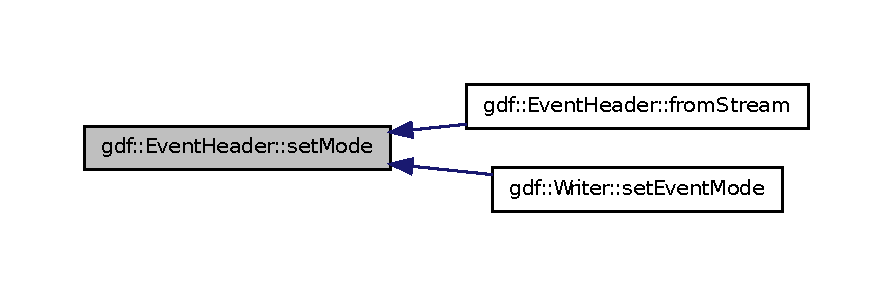
\includegraphics[width=400pt]{classgdf_1_1_event_header_a7384f73f64a72bb3c4a8a30423f8c1fd_icgraph}
\end{center}
\end{figure}


\hypertarget{classgdf_1_1_event_header_a2be9223eaf498c7d71ab0018205062b6}{
\index{gdf::EventHeader@{gdf::EventHeader}!setSamplingRate@{setSamplingRate}}
\index{setSamplingRate@{setSamplingRate}!gdf::EventHeader@{gdf::EventHeader}}
\subsubsection[{setSamplingRate}]{\setlength{\rightskip}{0pt plus 5cm}void gdf::EventHeader::setSamplingRate (
\begin{DoxyParamCaption}
\item[{float32}]{ fs}
\end{DoxyParamCaption}
)}}
\label{classgdf_1_1_event_header_a2be9223eaf498c7d71ab0018205062b6}


Set Sampling Rate associated with event positions. 

Events are not actually sampled, but their position is stored in samples rather than seconds. In order to convert event positions between time and sample, this sampling rate is used. 

Here is the caller graph for this function:
\nopagebreak
\begin{figure}[H]
\begin{center}
\leavevmode
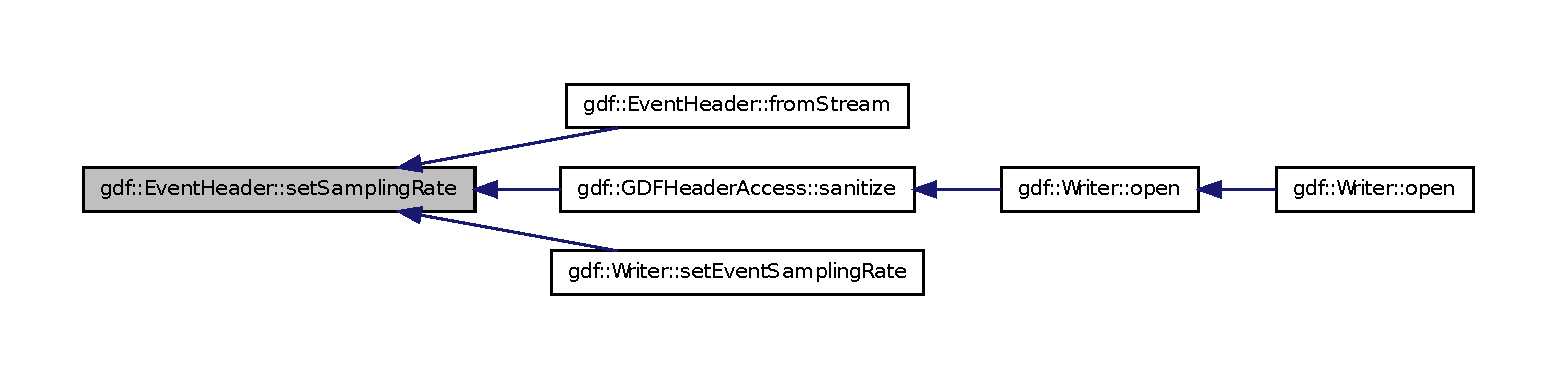
\includegraphics[width=400pt]{classgdf_1_1_event_header_a2be9223eaf498c7d71ab0018205062b6_icgraph}
\end{center}
\end{figure}




The documentation for this class was generated from the following files:\begin{DoxyCompactItemize}
\item 
include/GDF/EventHeader.h\item 
src/EventHeader.cpp\end{DoxyCompactItemize}

\hypertarget{classgdf_1_1exception_1_1feature__not__implemented}{
\section{gdf::exception::feature\_\-not\_\-implemented Class Reference}
\label{classgdf_1_1exception_1_1feature__not__implemented}\index{gdf::exception::feature\_\-not\_\-implemented@{gdf::exception::feature\_\-not\_\-implemented}}
}


Feature is not implemented yet.  




{\ttfamily \#include $<$Exceptions.h$>$}

\subsection*{Public Member Functions}
\begin{DoxyCompactItemize}
\item 
\hypertarget{classgdf_1_1exception_1_1feature__not__implemented_a0aaf9b8ec42a38423d1d6a3ec682e766}{
{\bfseries feature\_\-not\_\-implemented} (std::string str)}
\label{classgdf_1_1exception_1_1feature__not__implemented_a0aaf9b8ec42a38423d1d6a3ec682e766}

\end{DoxyCompactItemize}


\subsection{Detailed Description}
Feature is not implemented yet. 

The documentation for this class was generated from the following file:\begin{DoxyCompactItemize}
\item 
include/GDF/Exceptions.h\end{DoxyCompactItemize}

\hypertarget{classgdf_1_1exception_1_1file__exists}{
\section{gdf::exception::file\_\-exists Class Reference}
\label{classgdf_1_1exception_1_1file__exists}\index{gdf::exception::file\_\-exists@{gdf::exception::file\_\-exists}}
}


File exists.  




{\ttfamily \#include $<$Exceptions.h$>$}

\subsection*{Public Member Functions}
\begin{DoxyCompactItemize}
\item 
\hypertarget{classgdf_1_1exception_1_1file__exists_afaa7a02685aa12445cabf4c47ceece3e}{
{\bfseries file\_\-exists} (std::string str)}
\label{classgdf_1_1exception_1_1file__exists_afaa7a02685aa12445cabf4c47ceece3e}

\end{DoxyCompactItemize}


\subsection{Detailed Description}
File exists. 

The documentation for this class was generated from the following file:\begin{DoxyCompactItemize}
\item 
include/GDF/Exceptions.h\end{DoxyCompactItemize}

\hypertarget{classgdf_1_1exception_1_1file__exists__not}{
\section{gdf::exception::file\_\-exists\_\-not Class Reference}
\label{classgdf_1_1exception_1_1file__exists__not}\index{gdf::exception::file\_\-exists\_\-not@{gdf::exception::file\_\-exists\_\-not}}
}


File dos not exist.  




{\ttfamily \#include $<$Exceptions.h$>$}

\subsection*{Public Member Functions}
\begin{DoxyCompactItemize}
\item 
\hypertarget{classgdf_1_1exception_1_1file__exists__not_a6e60b81afdc785065f7250a9dac6c3f8}{
{\bfseries file\_\-exists\_\-not} (std::string str)}
\label{classgdf_1_1exception_1_1file__exists__not_a6e60b81afdc785065f7250a9dac6c3f8}

\end{DoxyCompactItemize}


\subsection{Detailed Description}
File dos not exist. 

The documentation for this class was generated from the following file:\begin{DoxyCompactItemize}
\item 
include/GDF/Exceptions.h\end{DoxyCompactItemize}

\hypertarget{classgdf_1_1exception_1_1file__not__open}{
\section{gdf::exception::file\_\-not\_\-open Class Reference}
\label{classgdf_1_1exception_1_1file__not__open}\index{gdf::exception::file\_\-not\_\-open@{gdf::exception::file\_\-not\_\-open}}
}


File is not open.  




{\ttfamily \#include $<$Exceptions.h$>$}

\subsection*{Public Member Functions}
\begin{DoxyCompactItemize}
\item 
\hypertarget{classgdf_1_1exception_1_1file__not__open_adc1b7f7e6b85dacda900d7144bac65a4}{
{\bfseries file\_\-not\_\-open} (std::string str)}
\label{classgdf_1_1exception_1_1file__not__open_adc1b7f7e6b85dacda900d7144bac65a4}

\end{DoxyCompactItemize}


\subsection{Detailed Description}
File is not open. 

The documentation for this class was generated from the following file:\begin{DoxyCompactItemize}
\item 
include/GDF/Exceptions.h\end{DoxyCompactItemize}

\hypertarget{classgdf_1_1_g_d_f_header_access}{
\section{gdf::GDFHeaderAccess Class Reference}
\label{classgdf_1_1_g_d_f_header_access}\index{gdf::GDFHeaderAccess@{gdf::GDFHeaderAccess}}
}


Collaboration diagram for gdf::GDFHeaderAccess:
\nopagebreak
\begin{figure}[H]
\begin{center}
\leavevmode
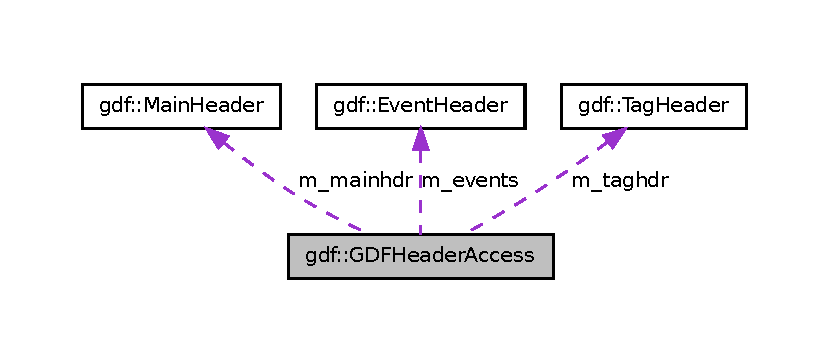
\includegraphics[width=398pt]{classgdf_1_1_g_d_f_header_access__coll__graph}
\end{center}
\end{figure}
\subsection*{Public Member Functions}
\begin{DoxyCompactItemize}
\item 
\hypertarget{classgdf_1_1_g_d_f_header_access_a12a8c246928d4f20a50ac6dea24e692f}{
\hyperlink{classgdf_1_1_g_d_f_header_access_a12a8c246928d4f20a50ac6dea24e692f}{GDFHeaderAccess} ()}
\label{classgdf_1_1_g_d_f_header_access_a12a8c246928d4f20a50ac6dea24e692f}

\begin{DoxyCompactList}\small\item\em Constructor. \item\end{DoxyCompactList}\item 
\hypertarget{classgdf_1_1_g_d_f_header_access_af05da736e9d7c18f9799c163fd595d3d}{
virtual \hyperlink{classgdf_1_1_g_d_f_header_access_af05da736e9d7c18f9799c163fd595d3d}{$\sim$GDFHeaderAccess} ()}
\label{classgdf_1_1_g_d_f_header_access_af05da736e9d7c18f9799c163fd595d3d}

\begin{DoxyCompactList}\small\item\em Destructor. \item\end{DoxyCompactList}\item 
\hypertarget{classgdf_1_1_g_d_f_header_access_abcc7802343db18a8c33d9a3c0bb26b43}{
void \hyperlink{classgdf_1_1_g_d_f_header_access_abcc7802343db18a8c33d9a3c0bb26b43}{clear} ()}
\label{classgdf_1_1_g_d_f_header_access_abcc7802343db18a8c33d9a3c0bb26b43}

\begin{DoxyCompactList}\small\item\em Reset header to initial state. \item\end{DoxyCompactList}\item 
void \hyperlink{classgdf_1_1_g_d_f_header_access_a16f91d1cb964f0acd3c842cf87c9d959}{sanitize} ()
\begin{DoxyCompactList}\small\item\em perform sanity check on header and normalize header information. \item\end{DoxyCompactList}\item 
void \hyperlink{classgdf_1_1_g_d_f_header_access_a116bd9d2057604f6894dae69ebb650ec}{setRecordDuration} (uint32 num, uint32 den)
\begin{DoxyCompactList}\small\item\em set record duration \item\end{DoxyCompactList}\item 
\hypertarget{classgdf_1_1_g_d_f_header_access_ad239f32a736961911c214130d1ba27fb}{
void \hyperlink{classgdf_1_1_g_d_f_header_access_ad239f32a736961911c214130d1ba27fb}{enableAutoRecordDuration} ()}
\label{classgdf_1_1_g_d_f_header_access_ad239f32a736961911c214130d1ba27fb}

\begin{DoxyCompactList}\small\item\em enable automatic record duration \item\end{DoxyCompactList}\item 
\hypertarget{classgdf_1_1_g_d_f_header_access_a83c19c8e3984ea3373a9eff57d9417d6}{
const \hyperlink{classgdf_1_1_main_header}{MainHeader} \& {\bfseries getMainHeader\_\-readonly} () const }
\label{classgdf_1_1_g_d_f_header_access_a83c19c8e3984ea3373a9eff57d9417d6}

\item 
\hypertarget{classgdf_1_1_g_d_f_header_access_af5ad6f26f1cf3b2db86cf08fd51316ac}{
\hyperlink{classgdf_1_1_main_header}{MainHeader} \& {\bfseries getMainHeader} ()}
\label{classgdf_1_1_g_d_f_header_access_af5ad6f26f1cf3b2db86cf08fd51316ac}

\item 
\hypertarget{classgdf_1_1_g_d_f_header_access_aa654d1657093402ec458e47ba7518f81}{
const \hyperlink{classgdf_1_1_signal_header}{SignalHeader} \& {\bfseries getSignalHeader\_\-readonly} (size\_\-t idx) const }
\label{classgdf_1_1_g_d_f_header_access_aa654d1657093402ec458e47ba7518f81}

\item 
\hypertarget{classgdf_1_1_g_d_f_header_access_a148a1ae5e2392fe01f8507bcaa01d640}{
\hyperlink{classgdf_1_1_signal_header}{SignalHeader} \& {\bfseries getSignalHeader} (size\_\-t idx)}
\label{classgdf_1_1_g_d_f_header_access_a148a1ae5e2392fe01f8507bcaa01d640}

\item 
\hypertarget{classgdf_1_1_g_d_f_header_access_a839d121ae6eef7957b40bce3c94ace59}{
bool {\bfseries createSignal} (size\_\-t index, bool throwexc=false)}
\label{classgdf_1_1_g_d_f_header_access_a839d121ae6eef7957b40bce3c94ace59}

\item 
\hypertarget{classgdf_1_1_g_d_f_header_access_a153f525fefd16cdd081f7b0608c1a55b}{
size\_\-t {\bfseries getFirstFreeSignalIndex} ()}
\label{classgdf_1_1_g_d_f_header_access_a153f525fefd16cdd081f7b0608c1a55b}

\item 
\hypertarget{classgdf_1_1_g_d_f_header_access_ad6352ce5ccbeb9221353822056e32651}{
size\_\-t {\bfseries getNumSignals} () const }
\label{classgdf_1_1_g_d_f_header_access_ad6352ce5ccbeb9221353822056e32651}

\item 
\hypertarget{classgdf_1_1_g_d_f_header_access_a39608e2b25e30765ed88278c66194383}{
void {\bfseries swapSignals} (size\_\-t a, size\_\-t b)}
\label{classgdf_1_1_g_d_f_header_access_a39608e2b25e30765ed88278c66194383}

\item 
\hypertarget{classgdf_1_1_g_d_f_header_access_a2792c0cf7366b9cebc82fd678aca39d6}{
void {\bfseries relocateSignal} (size\_\-t src, size\_\-t dst)}
\label{classgdf_1_1_g_d_f_header_access_a2792c0cf7366b9cebc82fd678aca39d6}

\item 
\hypertarget{classgdf_1_1_g_d_f_header_access_aabd8f13f27a8adc2de36a356b3674c07}{
\hyperlink{classgdf_1_1_event_header}{EventHeader} \& {\bfseries getEventHeader} ()}
\label{classgdf_1_1_g_d_f_header_access_aabd8f13f27a8adc2de36a356b3674c07}

\item 
\hypertarget{classgdf_1_1_g_d_f_header_access_a7e27e4527cebe030b3fd268defbeb95f}{
void \hyperlink{classgdf_1_1_g_d_f_header_access_a7e27e4527cebe030b3fd268defbeb95f}{setLock} (bool b)}
\label{classgdf_1_1_g_d_f_header_access_a7e27e4527cebe030b3fd268defbeb95f}

\begin{DoxyCompactList}\small\item\em Lock write access to headers. \item\end{DoxyCompactList}\end{DoxyCompactItemize}
\subsection*{Friends}
\begin{DoxyCompactItemize}
\item 
\hypertarget{classgdf_1_1_g_d_f_header_access_a0dd6213f6ada6c22b9c2e8e7890305a2}{
std::ostream \& \hyperlink{classgdf_1_1_g_d_f_header_access_a0dd6213f6ada6c22b9c2e8e7890305a2}{operator$<$$<$} (std::ostream \&out, const \hyperlink{classgdf_1_1_g_d_f_header_access}{GDFHeaderAccess} \&hdr)}
\label{classgdf_1_1_g_d_f_header_access_a0dd6213f6ada6c22b9c2e8e7890305a2}

\begin{DoxyCompactList}\small\item\em Header Serializer. \item\end{DoxyCompactList}\item 
\hypertarget{classgdf_1_1_g_d_f_header_access_a0a4dea8648fdd7b1131f900f772d2961}{
std::istream \& \hyperlink{classgdf_1_1_g_d_f_header_access_a0a4dea8648fdd7b1131f900f772d2961}{operator$>$$>$} (std::istream \&in, \hyperlink{classgdf_1_1_g_d_f_header_access}{GDFHeaderAccess} \&hdr)}
\label{classgdf_1_1_g_d_f_header_access_a0a4dea8648fdd7b1131f900f772d2961}

\begin{DoxyCompactList}\small\item\em Header Deserializer. \item\end{DoxyCompactList}\end{DoxyCompactItemize}


\subsection{Member Function Documentation}
\hypertarget{classgdf_1_1_g_d_f_header_access_a16f91d1cb964f0acd3c842cf87c9d959}{
\index{gdf::GDFHeaderAccess@{gdf::GDFHeaderAccess}!sanitize@{sanitize}}
\index{sanitize@{sanitize}!gdf::GDFHeaderAccess@{gdf::GDFHeaderAccess}}
\subsubsection[{sanitize}]{\setlength{\rightskip}{0pt plus 5cm}void gdf::GDFHeaderAccess::sanitize (
\begin{DoxyParamCaption}
{}
\end{DoxyParamCaption}
)}}
\label{classgdf_1_1_g_d_f_header_access_a16f91d1cb964f0acd3c842cf87c9d959}


perform sanity check on header and normalize header information. 

If there are issues with the configuration an exception with detailed information is thrown. 

Here is the call graph for this function:
\nopagebreak
\begin{figure}[H]
\begin{center}
\leavevmode
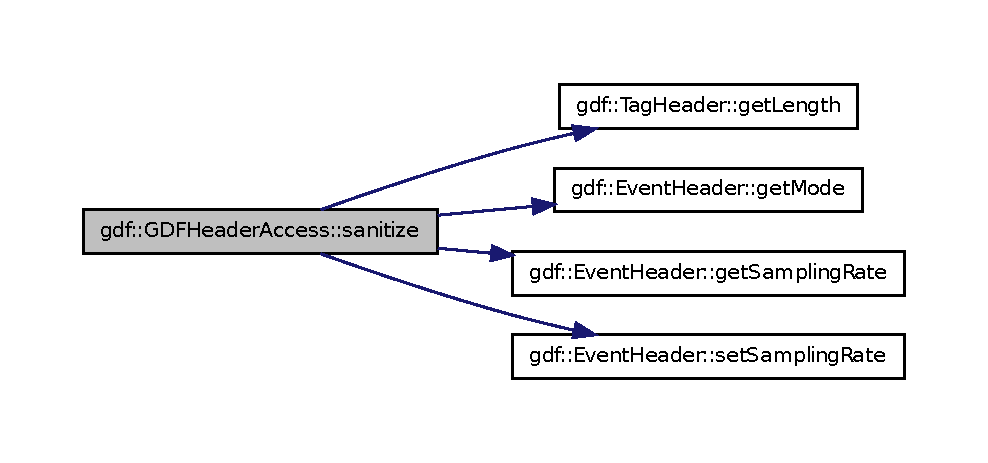
\includegraphics[width=400pt]{classgdf_1_1_g_d_f_header_access_a16f91d1cb964f0acd3c842cf87c9d959_cgraph}
\end{center}
\end{figure}




Here is the caller graph for this function:
\nopagebreak
\begin{figure}[H]
\begin{center}
\leavevmode
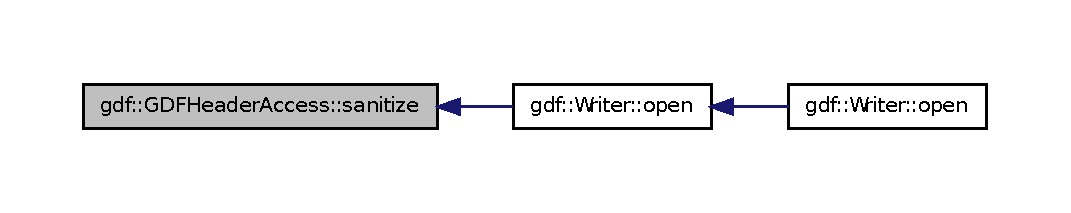
\includegraphics[width=400pt]{classgdf_1_1_g_d_f_header_access_a16f91d1cb964f0acd3c842cf87c9d959_icgraph}
\end{center}
\end{figure}


\hypertarget{classgdf_1_1_g_d_f_header_access_a116bd9d2057604f6894dae69ebb650ec}{
\index{gdf::GDFHeaderAccess@{gdf::GDFHeaderAccess}!setRecordDuration@{setRecordDuration}}
\index{setRecordDuration@{setRecordDuration}!gdf::GDFHeaderAccess@{gdf::GDFHeaderAccess}}
\subsubsection[{setRecordDuration}]{\setlength{\rightskip}{0pt plus 5cm}void gdf::GDFHeaderAccess::setRecordDuration (
\begin{DoxyParamCaption}
\item[{uint32}]{ num, }
\item[{uint32}]{ den}
\end{DoxyParamCaption}
)}}
\label{classgdf_1_1_g_d_f_header_access_a116bd9d2057604f6894dae69ebb650ec}


set record duration 

Normally record duration is automatically set to the smallest possible value. This functionality is overriden when manually setting the record duration. 

The documentation for this class was generated from the following files:\begin{DoxyCompactItemize}
\item 
include/GDF/GDFHeaderAccess.h\item 
src/GDFHeaderAccess.cpp\end{DoxyCompactItemize}

\hypertarget{classgdf_1_1exception_1_1general}{
\section{gdf::exception::general Class Reference}
\label{classgdf_1_1exception_1_1general}\index{gdf::exception::general@{gdf::exception::general}}
}


A general exception.  




{\ttfamily \#include $<$Exceptions.h$>$}

\subsection*{Public Member Functions}
\begin{DoxyCompactItemize}
\item 
\hypertarget{classgdf_1_1exception_1_1general_af54cd67a3c4dd8808176ea58567ddd0c}{
{\bfseries general} (const std::string str)}
\label{classgdf_1_1exception_1_1general_af54cd67a3c4dd8808176ea58567ddd0c}

\item 
\hypertarget{classgdf_1_1exception_1_1general_afcf154332d052569220eec9289d99604}{
const char $\ast$ {\bfseries what} () const   throw ()}
\label{classgdf_1_1exception_1_1general_afcf154332d052569220eec9289d99604}

\end{DoxyCompactItemize}


\subsection{Detailed Description}
A general exception. 

The documentation for this class was generated from the following file:\begin{DoxyCompactItemize}
\item 
include/GDF/Exceptions.h\end{DoxyCompactItemize}

\hypertarget{classgdf_1_1exception_1_1header__issues}{
\section{gdf::exception::header\_\-issues Class Reference}
\label{classgdf_1_1exception_1_1header__issues}\index{gdf::exception::header\_\-issues@{gdf::exception::header\_\-issues}}
}


Header Issues.  




{\ttfamily \#include $<$Exceptions.h$>$}

\subsection*{Public Member Functions}
\begin{DoxyCompactItemize}
\item 
\hypertarget{classgdf_1_1exception_1_1header__issues_a51dfee5a7b2b1b3965d52946bf620544}{
{\bfseries header\_\-issues} (std::list$<$ std::string $>$ w, std::list$<$ std::string $>$ e)}
\label{classgdf_1_1exception_1_1header__issues_a51dfee5a7b2b1b3965d52946bf620544}

\item 
\hypertarget{classgdf_1_1exception_1_1header__issues_a0bb44f875a6abadbbb50665da7341064}{
{\bfseries header\_\-issues} (std::list$<$ std::string $>$ w)}
\label{classgdf_1_1exception_1_1header__issues_a0bb44f875a6abadbbb50665da7341064}

\item 
\hypertarget{classgdf_1_1exception_1_1header__issues_a4fd481b2e3024733ed3b10cc2a3dd03e}{
const char $\ast$ {\bfseries what} () const   throw ()}
\label{classgdf_1_1exception_1_1header__issues_a4fd481b2e3024733ed3b10cc2a3dd03e}

\end{DoxyCompactItemize}
\subsection*{Public Attributes}
\begin{DoxyCompactItemize}
\item 
\hypertarget{classgdf_1_1exception_1_1header__issues_acd440727fb354287dc7b813809761641}{
std::list$<$ std::string $>$ {\bfseries warnings}}
\label{classgdf_1_1exception_1_1header__issues_acd440727fb354287dc7b813809761641}

\item 
\hypertarget{classgdf_1_1exception_1_1header__issues_a967348333d33a93388b0cee0d94c6814}{
std::list$<$ std::string $>$ {\bfseries errors}}
\label{classgdf_1_1exception_1_1header__issues_a967348333d33a93388b0cee0d94c6814}

\end{DoxyCompactItemize}


\subsection{Detailed Description}
Header Issues. 

The documentation for this class was generated from the following file:\begin{DoxyCompactItemize}
\item 
include/GDF/Exceptions.h\end{DoxyCompactItemize}

\hypertarget{structgdf_1_1_header_array}{
\section{gdf::HeaderArray$<$ T, P, L $>$ Struct Template Reference}
\label{structgdf_1_1_header_array}\index{gdf::HeaderArray@{gdf::HeaderArray}}
}


Store array-\/style header variable of length L and type T at offset P.  




{\ttfamily \#include $<$HeaderItem.h$>$}



Inherits \hyperlink{structgdf_1_1_header_item_base}{gdf::HeaderItemBase}.



Collaboration diagram for gdf::HeaderArray$<$ T, P, L $>$:
\nopagebreak
\begin{figure}[H]
\begin{center}
\leavevmode
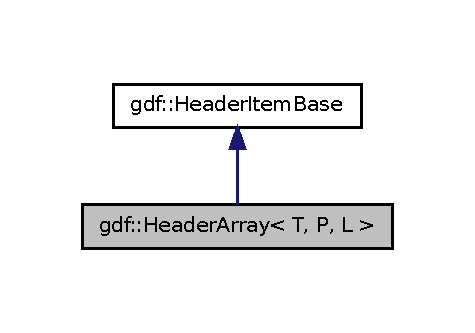
\includegraphics[width=228pt]{structgdf_1_1_header_array__coll__graph}
\end{center}
\end{figure}
\subsection*{Public Member Functions}
\begin{DoxyCompactItemize}
\item 
\hypertarget{structgdf_1_1_header_array_adddb102068fd68a0b7716cd9d64f2632}{
T \& {\bfseries operator\mbox{[}$\,$\mbox{]}} (size\_\-t idx)}
\label{structgdf_1_1_header_array_adddb102068fd68a0b7716cd9d64f2632}

\item 
\hypertarget{structgdf_1_1_header_array_ab336e83345a08541e45e86955c8d99e9}{
void {\bfseries tostream} (std::ostream \&out) const }
\label{structgdf_1_1_header_array_ab336e83345a08541e45e86955c8d99e9}

\item 
\hypertarget{structgdf_1_1_header_array_a249dba3a397de6f89b0a5e0c7c8257c0}{
void {\bfseries fromstream} (std::istream \&in)}
\label{structgdf_1_1_header_array_a249dba3a397de6f89b0a5e0c7c8257c0}

\end{DoxyCompactItemize}
\subsection*{Public Attributes}
\begin{DoxyCompactItemize}
\item 
\hypertarget{structgdf_1_1_header_array_a872bbeea5c9738988e8f703633f7a27b}{
T {\bfseries item} \mbox{[}L\mbox{]}}
\label{structgdf_1_1_header_array_a872bbeea5c9738988e8f703633f7a27b}

\item 
\hypertarget{structgdf_1_1_header_array_a851b8d7f5ca7098342cca6172ff67d8d}{
size\_\-t {\bfseries pos}}
\label{structgdf_1_1_header_array_a851b8d7f5ca7098342cca6172ff67d8d}

\item 
\hypertarget{structgdf_1_1_header_array_acbb388bc7b071bfd3b578f1740eb81ee}{
size\_\-t {\bfseries len}}
\label{structgdf_1_1_header_array_acbb388bc7b071bfd3b578f1740eb81ee}

\end{DoxyCompactItemize}


\subsection{Detailed Description}
\subsubsection*{template$<$typename T, size\_\-t P, size\_\-t L$>$ struct gdf::HeaderArray$<$ T, P, L $>$}

Store array-\/style header variable of length L and type T at offset P. 

The documentation for this struct was generated from the following file:\begin{DoxyCompactItemize}
\item 
include/GDF/HeaderItem.h\end{DoxyCompactItemize}

\hypertarget{structgdf_1_1_header_item}{
\section{gdf::HeaderItem$<$ T, P $>$ Struct Template Reference}
\label{structgdf_1_1_header_item}\index{gdf::HeaderItem@{gdf::HeaderItem}}
}


Store header variable of type T at offset P.  




{\ttfamily \#include $<$HeaderItem.h$>$}



Inherits \hyperlink{structgdf_1_1_header_item_base}{gdf::HeaderItemBase}.



Collaboration diagram for gdf::HeaderItem$<$ T, P $>$:
\nopagebreak
\begin{figure}[H]
\begin{center}
\leavevmode
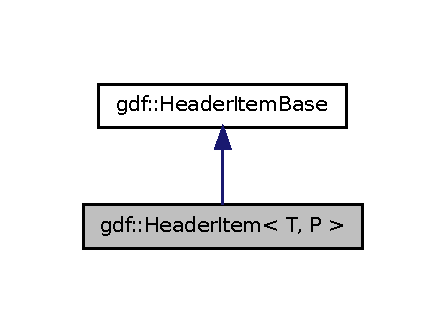
\includegraphics[width=214pt]{structgdf_1_1_header_item__coll__graph}
\end{center}
\end{figure}
\subsection*{Public Member Functions}
\begin{DoxyCompactItemize}
\item 
\hypertarget{structgdf_1_1_header_item_ab42a9a6c269c8017bda2c3fad2e7f380}{
void {\bfseries tostream} (std::ostream \&out) const }
\label{structgdf_1_1_header_item_ab42a9a6c269c8017bda2c3fad2e7f380}

\item 
\hypertarget{structgdf_1_1_header_item_af5858887d1a71550ef9b075bea208f9e}{
void {\bfseries fromstream} (std::istream \&in)}
\label{structgdf_1_1_header_item_af5858887d1a71550ef9b075bea208f9e}

\end{DoxyCompactItemize}
\subsection*{Public Attributes}
\begin{DoxyCompactItemize}
\item 
\hypertarget{structgdf_1_1_header_item_a9b7e1442ba79f8d4fb64955b397ce79f}{
T {\bfseries item}}
\label{structgdf_1_1_header_item_a9b7e1442ba79f8d4fb64955b397ce79f}

\item 
\hypertarget{structgdf_1_1_header_item_ad92b903a032ea69589c789a52dd19021}{
size\_\-t {\bfseries pos}}
\label{structgdf_1_1_header_item_ad92b903a032ea69589c789a52dd19021}

\end{DoxyCompactItemize}


\subsection{Detailed Description}
\subsubsection*{template$<$typename T, size\_\-t P$>$ struct gdf::HeaderItem$<$ T, P $>$}

Store header variable of type T at offset P. 

The documentation for this struct was generated from the following file:\begin{DoxyCompactItemize}
\item 
include/GDF/HeaderItem.h\end{DoxyCompactItemize}

\hypertarget{structgdf_1_1_header_item_base}{
\section{gdf::HeaderItemBase Struct Reference}
\label{structgdf_1_1_header_item_base}\index{gdf::HeaderItemBase@{gdf::HeaderItemBase}}
}


Inherited by \hyperlink{structgdf_1_1_header_array}{gdf::HeaderArray$<$ T, P, L $>$}, and \hyperlink{structgdf_1_1_header_item}{gdf::HeaderItem$<$ T, P $>$}.

\subsection*{Public Member Functions}
\begin{DoxyCompactItemize}
\item 
\hypertarget{structgdf_1_1_header_item_base_a2e31b4b08ee7131198881a9f6b05af68}{
virtual void {\bfseries tostream} (std::ostream \&out) const =0}
\label{structgdf_1_1_header_item_base_a2e31b4b08ee7131198881a9f6b05af68}

\end{DoxyCompactItemize}


The documentation for this struct was generated from the following file:\begin{DoxyCompactItemize}
\item 
include/GDF/HeaderItem.h\end{DoxyCompactItemize}

\hypertarget{structgdf_1_1_header_ref}{
\section{gdf::HeaderRef Struct Reference}
\label{structgdf_1_1_header_ref}\index{gdf::HeaderRef@{gdf::HeaderRef}}
}
\subsection*{Public Member Functions}
\begin{DoxyCompactItemize}
\item 
\hypertarget{structgdf_1_1_header_ref_a77d569b72d944639f9b2d8b83260cec7}{
{\bfseries HeaderRef} (std::string n=\char`\"{}\char`\"{}, void $\ast$r=NULL, size\_\-t o=0, size\_\-t l=0)}
\label{structgdf_1_1_header_ref_a77d569b72d944639f9b2d8b83260cec7}

\end{DoxyCompactItemize}
\subsection*{Public Attributes}
\begin{DoxyCompactItemize}
\item 
\hypertarget{structgdf_1_1_header_ref_a19f94b2d3a392ae1790c2b463b4d09af}{
std::string {\bfseries name}}
\label{structgdf_1_1_header_ref_a19f94b2d3a392ae1790c2b463b4d09af}

\item 
\hypertarget{structgdf_1_1_header_ref_afa9d3f2d40585bfe74a923b31c656b8a}{
void $\ast$ {\bfseries ref}}
\label{structgdf_1_1_header_ref_afa9d3f2d40585bfe74a923b31c656b8a}

\item 
\hypertarget{structgdf_1_1_header_ref_ad9fe9768e64fcc7bb1c3c01e617ea315}{
size\_\-t {\bfseries ofs}}
\label{structgdf_1_1_header_ref_ad9fe9768e64fcc7bb1c3c01e617ea315}

\item 
\hypertarget{structgdf_1_1_header_ref_a1125928773f5b087849fb07ec6aeb8e3}{
size\_\-t {\bfseries len}}
\label{structgdf_1_1_header_ref_a1125928773f5b087849fb07ec6aeb8e3}

\end{DoxyCompactItemize}


The documentation for this struct was generated from the following file:\begin{DoxyCompactItemize}
\item 
include/GDF/HeaderItem.h\end{DoxyCompactItemize}

\hypertarget{classgdf_1_1exception_1_1illegal__eventmode__change}{
\section{gdf::exception::illegal\_\-eventmode\_\-change Class Reference}
\label{classgdf_1_1exception_1_1illegal__eventmode__change}\index{gdf::exception::illegal\_\-eventmode\_\-change@{gdf::exception::illegal\_\-eventmode\_\-change}}
}


Illegal attempt to change event mode.  




{\ttfamily \#include $<$Exceptions.h$>$}

\subsection*{Public Member Functions}
\begin{DoxyCompactItemize}
\item 
\hypertarget{classgdf_1_1exception_1_1illegal__eventmode__change_ade675c9801b3f6cf5f8664a41b13abfb}{
{\bfseries illegal\_\-eventmode\_\-change} (std::string str)}
\label{classgdf_1_1exception_1_1illegal__eventmode__change_ade675c9801b3f6cf5f8664a41b13abfb}

\end{DoxyCompactItemize}


\subsection{Detailed Description}
Illegal attempt to change event mode. 

The documentation for this class was generated from the following file:\begin{DoxyCompactItemize}
\item 
include/GDF/Exceptions.h\end{DoxyCompactItemize}

\hypertarget{classgdf_1_1exception_1_1index__out__of__range}{
\section{gdf::exception::index\_\-out\_\-of\_\-range Class Reference}
\label{classgdf_1_1exception_1_1index__out__of__range}\index{gdf::exception::index\_\-out\_\-of\_\-range@{gdf::exception::index\_\-out\_\-of\_\-range}}
}


An index exceeds it's valid range.  




{\ttfamily \#include $<$Exceptions.h$>$}

\subsection*{Public Member Functions}
\begin{DoxyCompactItemize}
\item 
\hypertarget{classgdf_1_1exception_1_1index__out__of__range_a71007b84649cdf333ef61f35969aa9d3}{
{\bfseries index\_\-out\_\-of\_\-range} (std::string str)}
\label{classgdf_1_1exception_1_1index__out__of__range_a71007b84649cdf333ef61f35969aa9d3}

\end{DoxyCompactItemize}


\subsection{Detailed Description}
An index exceeds it's valid range. 

The documentation for this class was generated from the following file:\begin{DoxyCompactItemize}
\item 
include/GDF/Exceptions.h\end{DoxyCompactItemize}

\hypertarget{classgdf_1_1exception_1_1invalid__eventmode}{
\section{gdf::exception::invalid\_\-eventmode Class Reference}
\label{classgdf_1_1exception_1_1invalid__eventmode}\index{gdf::exception::invalid\_\-eventmode@{gdf::exception::invalid\_\-eventmode}}
}


Invalid event mode.  




{\ttfamily \#include $<$Exceptions.h$>$}

\subsection*{Public Member Functions}
\begin{DoxyCompactItemize}
\item 
\hypertarget{classgdf_1_1exception_1_1invalid__eventmode_ae26137abe6427cc826f03afb261adf8f}{
{\bfseries invalid\_\-eventmode} (std::string str)}
\label{classgdf_1_1exception_1_1invalid__eventmode_ae26137abe6427cc826f03afb261adf8f}

\end{DoxyCompactItemize}


\subsection{Detailed Description}
Invalid event mode. 

The documentation for this class was generated from the following file:\begin{DoxyCompactItemize}
\item 
include/GDF/Exceptions.h\end{DoxyCompactItemize}

\hypertarget{classgdf_1_1exception_1_1invalid__operation}{
\section{gdf::exception::invalid\_\-operation Class Reference}
\label{classgdf_1_1exception_1_1invalid__operation}\index{gdf::exception::invalid\_\-operation@{gdf::exception::invalid\_\-operation}}
}


Preconditions for operation are not met.  




{\ttfamily \#include $<$Exceptions.h$>$}

\subsection*{Public Member Functions}
\begin{DoxyCompactItemize}
\item 
\hypertarget{classgdf_1_1exception_1_1invalid__operation_a6f9994c824ca966fa82c4650233e7626}{
{\bfseries invalid\_\-operation} (std::string str)}
\label{classgdf_1_1exception_1_1invalid__operation_a6f9994c824ca966fa82c4650233e7626}

\end{DoxyCompactItemize}


\subsection{Detailed Description}
Preconditions for operation are not met. 

The documentation for this class was generated from the following file:\begin{DoxyCompactItemize}
\item 
include/GDF/Exceptions.h\end{DoxyCompactItemize}

\hypertarget{classgdf_1_1exception_1_1invalid__type__id}{
\section{gdf::exception::invalid\_\-type\_\-id Class Reference}
\label{classgdf_1_1exception_1_1invalid__type__id}\index{gdf::exception::invalid\_\-type\_\-id@{gdf::exception::invalid\_\-type\_\-id}}
}


Type ID used is not defined in \hyperlink{_types_8h_source}{Types.h}.  




{\ttfamily \#include $<$Exceptions.h$>$}

\subsection*{Public Member Functions}
\begin{DoxyCompactItemize}
\item 
\hypertarget{classgdf_1_1exception_1_1invalid__type__id_a2bfa052162e285ba621cae88068f3783}{
{\bfseries invalid\_\-type\_\-id} (std::string str)}
\label{classgdf_1_1exception_1_1invalid__type__id_a2bfa052162e285ba621cae88068f3783}

\end{DoxyCompactItemize}


\subsection{Detailed Description}
Type ID used is not defined in \hyperlink{_types_8h_source}{Types.h}. 

The documentation for this class was generated from the following file:\begin{DoxyCompactItemize}
\item 
include/GDF/Exceptions.h\end{DoxyCompactItemize}

\hypertarget{classgdf_1_1_main_header}{
\section{gdf::MainHeader Class Reference}
\label{classgdf_1_1_main_header}\index{gdf::MainHeader@{gdf::MainHeader}}
}


Contains all information required to construct the GDF fixed header.  




{\ttfamily \#include $<$MainHeader.h$>$}

\subsection*{Friends}
\begin{DoxyCompactItemize}
\item 
\hypertarget{classgdf_1_1_main_header_ade47bf1d3f5a91747dd7fbb489fbcab0}{
class {\bfseries GDFHeaderAccess}}
\label{classgdf_1_1_main_header_ade47bf1d3f5a91747dd7fbb489fbcab0}

\item 
\hypertarget{classgdf_1_1_main_header_ab699d593c3b9dee1ed8d700a93d70700}{
class {\bfseries Writer}}
\label{classgdf_1_1_main_header_ab699d593c3b9dee1ed8d700a93d70700}

\item 
\hypertarget{classgdf_1_1_main_header_a35cb182752752c74a30050705acc3c06}{
class {\bfseries Reader}}
\label{classgdf_1_1_main_header_a35cb182752752c74a30050705acc3c06}

\item 
\hypertarget{classgdf_1_1_main_header_a0dd6213f6ada6c22b9c2e8e7890305a2}{
std::ostream \& \hyperlink{classgdf_1_1_main_header_a0dd6213f6ada6c22b9c2e8e7890305a2}{operator$<$$<$} (std::ostream \&out, const \hyperlink{classgdf_1_1_g_d_f_header_access}{GDFHeaderAccess} \&hdr)}
\label{classgdf_1_1_main_header_a0dd6213f6ada6c22b9c2e8e7890305a2}

\begin{DoxyCompactList}\small\item\em Header Serializer. \item\end{DoxyCompactList}\item 
\hypertarget{classgdf_1_1_main_header_a0a4dea8648fdd7b1131f900f772d2961}{
std::istream \& \hyperlink{classgdf_1_1_main_header_a0a4dea8648fdd7b1131f900f772d2961}{operator$>$$>$} (std::istream \&in, \hyperlink{classgdf_1_1_g_d_f_header_access}{GDFHeaderAccess} \&hdr)}
\label{classgdf_1_1_main_header_a0a4dea8648fdd7b1131f900f772d2961}

\begin{DoxyCompactList}\small\item\em Header Deserializer. \item\end{DoxyCompactList}\end{DoxyCompactItemize}


\subsection{Detailed Description}
Contains all information required to construct the GDF fixed header. 

The documentation for this class was generated from the following file:\begin{DoxyCompactItemize}
\item 
include/GDF/MainHeader.h\end{DoxyCompactItemize}

\hypertarget{classgdf_1_1exception_1_1mismatch__channel__number}{
\section{gdf::exception::mismatch\_\-channel\_\-number Class Reference}
\label{classgdf_1_1exception_1_1mismatch__channel__number}\index{gdf::exception::mismatch\_\-channel\_\-number@{gdf::exception::mismatch\_\-channel\_\-number}}
}


Number of channels does not match.  




{\ttfamily \#include $<$Exceptions.h$>$}

\subsection*{Public Member Functions}
\begin{DoxyCompactItemize}
\item 
\hypertarget{classgdf_1_1exception_1_1mismatch__channel__number_ae918beb7c33758ffe1331d47905693c6}{
{\bfseries mismatch\_\-channel\_\-number} (std::string str)}
\label{classgdf_1_1exception_1_1mismatch__channel__number_ae918beb7c33758ffe1331d47905693c6}

\end{DoxyCompactItemize}


\subsection{Detailed Description}
Number of channels does not match. 

The documentation for this class was generated from the following file:\begin{DoxyCompactItemize}
\item 
include/GDF/Exceptions.h\end{DoxyCompactItemize}

\hypertarget{classgdf_1_1exception_1_1mixed__types__not__allowed}{
\section{gdf::exception::mixed\_\-types\_\-not\_\-allowed Class Reference}
\label{classgdf_1_1exception_1_1mixed__types__not__allowed}\index{gdf::exception::mixed\_\-types\_\-not\_\-allowed@{gdf::exception::mixed\_\-types\_\-not\_\-allowed}}
}


Channels of different types were used where it's not allowed.  




{\ttfamily \#include $<$Exceptions.h$>$}

\subsection*{Public Member Functions}
\begin{DoxyCompactItemize}
\item 
\hypertarget{classgdf_1_1exception_1_1mixed__types__not__allowed_afedb67ea57a869c684df590bce99b18c}{
{\bfseries mixed\_\-types\_\-not\_\-allowed} (std::string str)}
\label{classgdf_1_1exception_1_1mixed__types__not__allowed_afedb67ea57a869c684df590bce99b18c}

\end{DoxyCompactItemize}


\subsection{Detailed Description}
Channels of different types were used where it's not allowed. 

The documentation for this class was generated from the following file:\begin{DoxyCompactItemize}
\item 
include/GDF/Exceptions.h\end{DoxyCompactItemize}

\hypertarget{structgdf_1_1_mode1_event}{
\section{gdf::Mode1Event Struct Reference}
\label{structgdf_1_1_mode1_event}\index{gdf::Mode1Event@{gdf::Mode1Event}}
}
\subsection*{Public Member Functions}
\begin{DoxyCompactItemize}
\item 
\hypertarget{structgdf_1_1_mode1_event_aa3c06e75446dba917c427d706952c407}{
bool {\bfseries operator$<$} (const \hyperlink{structgdf_1_1_mode1_event}{Mode1Event} \&e) const }
\label{structgdf_1_1_mode1_event_aa3c06e75446dba917c427d706952c407}

\end{DoxyCompactItemize}
\subsection*{Public Attributes}
\begin{DoxyCompactItemize}
\item 
\hypertarget{structgdf_1_1_mode1_event_a8e52848bd8d87dc2d609925c8eed0fa1}{
uint32 {\bfseries position}}
\label{structgdf_1_1_mode1_event_a8e52848bd8d87dc2d609925c8eed0fa1}

\item 
\hypertarget{structgdf_1_1_mode1_event_aa66f9619b5af94eaca1cfc9fc8de1c4d}{
uint16 {\bfseries type}}
\label{structgdf_1_1_mode1_event_aa66f9619b5af94eaca1cfc9fc8de1c4d}

\end{DoxyCompactItemize}


The documentation for this struct was generated from the following file:\begin{DoxyCompactItemize}
\item 
include/GDF/EventHeader.h\end{DoxyCompactItemize}

\hypertarget{structgdf_1_1_mode3_event}{
\section{gdf::Mode3Event Struct Reference}
\label{structgdf_1_1_mode3_event}\index{gdf::Mode3Event@{gdf::Mode3Event}}
}
\subsection*{Public Member Functions}
\begin{DoxyCompactItemize}
\item 
\hypertarget{structgdf_1_1_mode3_event_a195f242281c8f1f914127e650093e33b}{
bool {\bfseries operator$<$} (const \hyperlink{structgdf_1_1_mode3_event}{Mode3Event} \&e) const }
\label{structgdf_1_1_mode3_event_a195f242281c8f1f914127e650093e33b}

\end{DoxyCompactItemize}
\subsection*{Public Attributes}
\begin{DoxyCompactItemize}
\item 
\hypertarget{structgdf_1_1_mode3_event_a5d1e27568021143db0286f54d787d84b}{
uint32 {\bfseries position}}
\label{structgdf_1_1_mode3_event_a5d1e27568021143db0286f54d787d84b}

\item 
\hypertarget{structgdf_1_1_mode3_event_af62bac1fcff5a804a8070f1d7aa39beb}{
uint16 {\bfseries type}}
\label{structgdf_1_1_mode3_event_af62bac1fcff5a804a8070f1d7aa39beb}

\item 
\hypertarget{structgdf_1_1_mode3_event_a2b0337d816fd8f81d5b296b6e4c6b3dd}{
uint16 {\bfseries channel}}
\label{structgdf_1_1_mode3_event_a2b0337d816fd8f81d5b296b6e4c6b3dd}

\item 
\hypertarget{structgdf_1_1_mode3_event_af8dcc81248b5e18cb2989b42efa66ddf}{
\begin{tabbing}
xx\=xx\=xx\=xx\=xx\=xx\=xx\=xx\=xx\=\kill
union \{\\
\>uint32 {\bfseries duration}\\
\>float32 {\bfseries value}\\
\}; }
\label{structgdf_1_1_mode3_event_af8dcc81248b5e18cb2989b42efa66ddf}
\\

\end{tabbing}\end{DoxyCompactItemize}


The documentation for this struct was generated from the following file:\begin{DoxyCompactItemize}
\item 
include/GDF/EventHeader.h\end{DoxyCompactItemize}

\hypertarget{classgdf_1_1_modifier}{
\section{gdf::Modifier Class Reference}
\label{classgdf_1_1_modifier}\index{gdf::Modifier@{gdf::Modifier}}
}


Class for reading, modifying and saving changes to GDF files.  




{\ttfamily \#include $<$Modifier.h$>$}



Inherits \hyperlink{classgdf_1_1_reader}{gdf::Reader}.



Collaboration diagram for gdf::Modifier:
\nopagebreak
\begin{figure}[H]
\begin{center}
\leavevmode
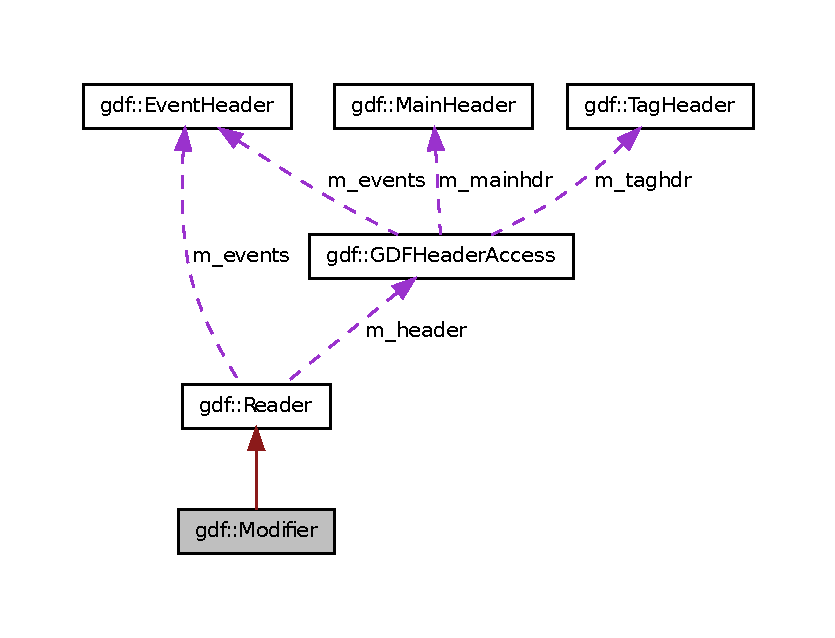
\includegraphics[width=400pt]{classgdf_1_1_modifier__coll__graph}
\end{center}
\end{figure}
\subsection*{Public Member Functions}
\begin{DoxyCompactItemize}
\item 
\hypertarget{classgdf_1_1_modifier_a6fe073392dcedae9fbdd084708afb1be}{
\hyperlink{classgdf_1_1_modifier_a6fe073392dcedae9fbdd084708afb1be}{Modifier} ()}
\label{classgdf_1_1_modifier_a6fe073392dcedae9fbdd084708afb1be}

\begin{DoxyCompactList}\small\item\em Constructor. \item\end{DoxyCompactList}\item 
\hypertarget{classgdf_1_1_modifier_a4def55c87a3bb26c3a51c59d76cca155}{
virtual \hyperlink{classgdf_1_1_modifier_a4def55c87a3bb26c3a51c59d76cca155}{$\sim$Modifier} ()}
\label{classgdf_1_1_modifier_a4def55c87a3bb26c3a51c59d76cca155}

\begin{DoxyCompactList}\small\item\em Destructor. \item\end{DoxyCompactList}\item 
\hypertarget{classgdf_1_1_modifier_abcb4c7bfa55babf4d1cc82b916877eda}{
void \hyperlink{classgdf_1_1_modifier_abcb4c7bfa55babf4d1cc82b916877eda}{open} (const std::string filename)}
\label{classgdf_1_1_modifier_abcb4c7bfa55babf4d1cc82b916877eda}

\begin{DoxyCompactList}\small\item\em Opens file for modification. \item\end{DoxyCompactList}\item 
\hypertarget{classgdf_1_1_modifier_a11862cf81de237520bf969f2755a1a08}{
void \hyperlink{classgdf_1_1_modifier_a11862cf81de237520bf969f2755a1a08}{close} ()}
\label{classgdf_1_1_modifier_a11862cf81de237520bf969f2755a1a08}

\begin{DoxyCompactList}\small\item\em Close file. \item\end{DoxyCompactList}\item 
\hypertarget{classgdf_1_1_modifier_a88b582ab5f78daf05796c89397523f5b}{
void \hyperlink{classgdf_1_1_modifier_a88b582ab5f78daf05796c89397523f5b}{saveChanges} ()}
\label{classgdf_1_1_modifier_a88b582ab5f78daf05796c89397523f5b}

\begin{DoxyCompactList}\small\item\em Write changes to disk. \item\end{DoxyCompactList}\item 
double \hyperlink{classgdf_1_1_modifier_aa5d1ba80d46c3cd55f3930b586e57585}{getSample} (uint16 channel\_\-idx, size\_\-t sample\_\-idx)
\begin{DoxyCompactList}\small\item\em Get a single Sample (physical units). \item\end{DoxyCompactList}\item 
void \hyperlink{classgdf_1_1_modifier_a7466a9097151cbb0176936bc979d01d9}{setSample} (uint16 channel\_\-idx, size\_\-t sample\_\-idx, double value)
\begin{DoxyCompactList}\small\item\em Set a single Sample (physical units). \item\end{DoxyCompactList}\item 
\hypertarget{classgdf_1_1_modifier_ababfb7e1503c8030a821059a78980348}{
\hyperlink{classgdf_1_1_event_header}{EventHeader} $\ast$ \hyperlink{classgdf_1_1_modifier_ababfb7e1503c8030a821059a78980348}{getEventHeader} ()}
\label{classgdf_1_1_modifier_ababfb7e1503c8030a821059a78980348}

\begin{DoxyCompactList}\small\item\em get writable reference to event header \item\end{DoxyCompactList}\item 
\hypertarget{classgdf_1_1_modifier_a1067dfac1c4d09ebe5b892e6eee7ed81}{
const \hyperlink{classgdf_1_1_event_header}{EventHeader} $\ast$ \hyperlink{classgdf_1_1_modifier_a1067dfac1c4d09ebe5b892e6eee7ed81}{getEventHeader\_\-readonly} ()}
\label{classgdf_1_1_modifier_a1067dfac1c4d09ebe5b892e6eee7ed81}

\begin{DoxyCompactList}\small\item\em get const reference to event header \item\end{DoxyCompactList}\end{DoxyCompactItemize}


\subsection{Detailed Description}
Class for reading, modifying and saving changes to GDF files. It is not possible to change the number of signals or their length. When a sample is set, the entire record is marked for rewriting. If the Event Header is retrieved using the non-\/const get function, it is marked for rewriting. 

\subsection{Member Function Documentation}
\hypertarget{classgdf_1_1_modifier_aa5d1ba80d46c3cd55f3930b586e57585}{
\index{gdf::Modifier@{gdf::Modifier}!getSample@{getSample}}
\index{getSample@{getSample}!gdf::Modifier@{gdf::Modifier}}
\subsubsection[{getSample}]{\setlength{\rightskip}{0pt plus 5cm}double gdf::Modifier::getSample (
\begin{DoxyParamCaption}
\item[{uint16}]{ channel\_\-idx, }
\item[{size\_\-t}]{ sample\_\-idx}
\end{DoxyParamCaption}
)}}
\label{classgdf_1_1_modifier_aa5d1ba80d46c3cd55f3930b586e57585}


Get a single Sample (physical units). 


\begin{DoxyParams}{Parameters}
\item[\mbox{\tt[in]} {\em channel\_\-idx}]channel index \item[\mbox{\tt[in]} {\em sample\_\-idx}]sample index \end{DoxyParams}


Reimplemented from \hyperlink{classgdf_1_1_reader_ab0c56ba1256f76ac62663bd634fac79f}{gdf::Reader}.



Here is the call graph for this function:
\nopagebreak
\begin{figure}[H]
\begin{center}
\leavevmode
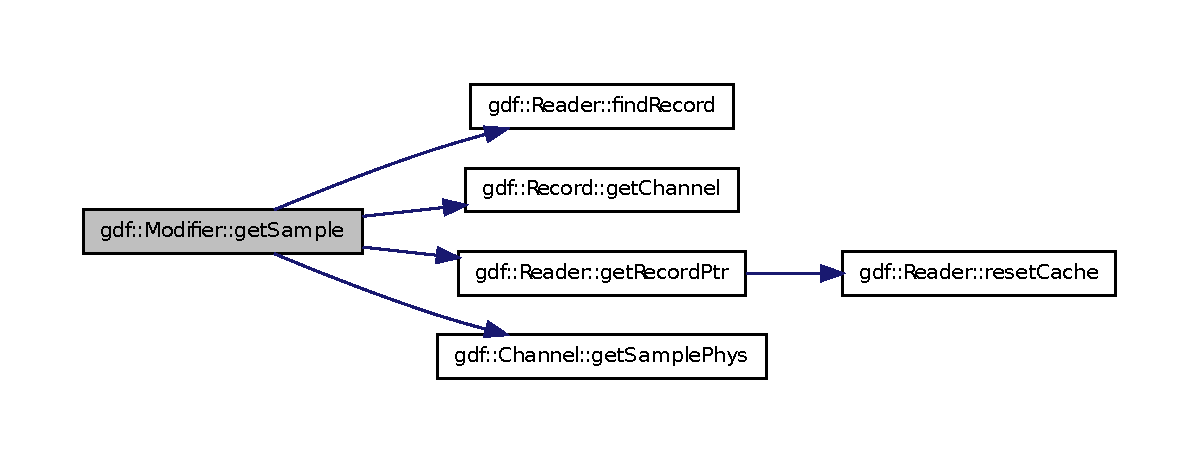
\includegraphics[width=400pt]{classgdf_1_1_modifier_aa5d1ba80d46c3cd55f3930b586e57585_cgraph}
\end{center}
\end{figure}


\hypertarget{classgdf_1_1_modifier_a7466a9097151cbb0176936bc979d01d9}{
\index{gdf::Modifier@{gdf::Modifier}!setSample@{setSample}}
\index{setSample@{setSample}!gdf::Modifier@{gdf::Modifier}}
\subsubsection[{setSample}]{\setlength{\rightskip}{0pt plus 5cm}void gdf::Modifier::setSample (
\begin{DoxyParamCaption}
\item[{uint16}]{ channel\_\-idx, }
\item[{size\_\-t}]{ sample\_\-idx, }
\item[{double}]{ value}
\end{DoxyParamCaption}
)}}
\label{classgdf_1_1_modifier_a7466a9097151cbb0176936bc979d01d9}


Set a single Sample (physical units). 


\begin{DoxyParams}{Parameters}
\item[\mbox{\tt[in]} {\em channel\_\-idx}]channel index \item[\mbox{\tt[in]} {\em sample\_\-idx}]sample index \item[\mbox{\tt[in]} {\em value}]\end{DoxyParams}


Here is the call graph for this function:
\nopagebreak
\begin{figure}[H]
\begin{center}
\leavevmode
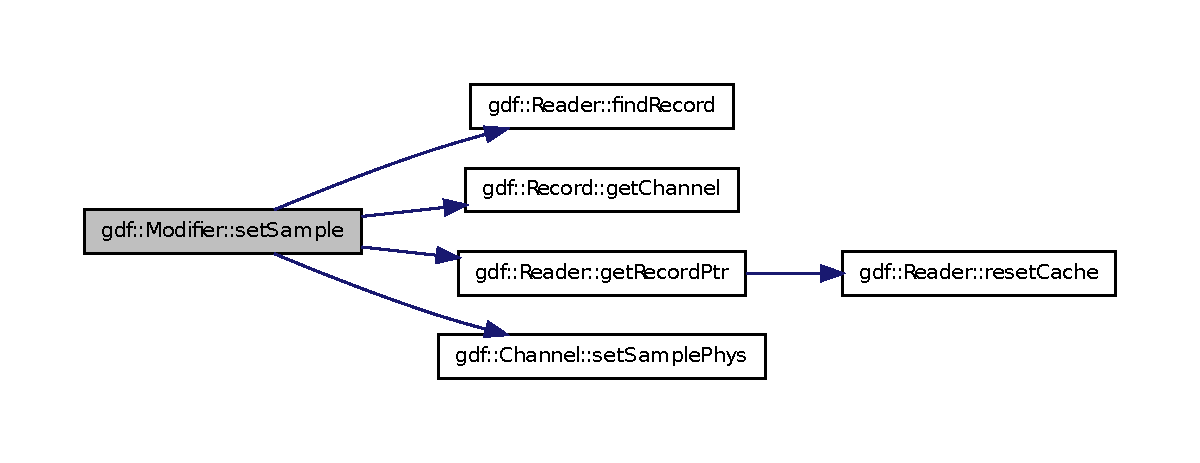
\includegraphics[width=400pt]{classgdf_1_1_modifier_a7466a9097151cbb0176936bc979d01d9_cgraph}
\end{center}
\end{figure}




The documentation for this class was generated from the following files:\begin{DoxyCompactItemize}
\item 
include/GDF/Modifier.h\item 
src/Modifier.cpp\end{DoxyCompactItemize}

\hypertarget{classgdf_1_1exception_1_1nonexistent__channel__access}{
\section{gdf::exception::nonexistent\_\-channel\_\-access Class Reference}
\label{classgdf_1_1exception_1_1nonexistent__channel__access}\index{gdf::exception::nonexistent\_\-channel\_\-access@{gdf::exception::nonexistent\_\-channel\_\-access}}
}


\hyperlink{classgdf_1_1_channel}{Channel} does not exist.  




{\ttfamily \#include $<$Exceptions.h$>$}

\subsection*{Public Member Functions}
\begin{DoxyCompactItemize}
\item 
\hypertarget{classgdf_1_1exception_1_1nonexistent__channel__access_ab93aea48db58492eff7e768086cee264}{
{\bfseries nonexistent\_\-channel\_\-access} (std::string str)}
\label{classgdf_1_1exception_1_1nonexistent__channel__access_ab93aea48db58492eff7e768086cee264}

\end{DoxyCompactItemize}


\subsection{Detailed Description}
\hyperlink{classgdf_1_1_channel}{Channel} does not exist. 

The documentation for this class was generated from the following file:\begin{DoxyCompactItemize}
\item 
include/GDF/Exceptions.h\end{DoxyCompactItemize}

\hypertarget{classgdf_1_1_reader}{
\section{gdf::Reader Class Reference}
\label{classgdf_1_1_reader}\index{gdf::Reader@{gdf::Reader}}
}


Class for reading GDF files to disc.  




{\ttfamily \#include $<$Reader.h$>$}



Inherited by \hyperlink{classgdf_1_1_modifier}{gdf::Modifier}{\ttfamily  \mbox{[}private\mbox{]}}.



Collaboration diagram for gdf::Reader:
\nopagebreak
\begin{figure}[H]
\begin{center}
\leavevmode
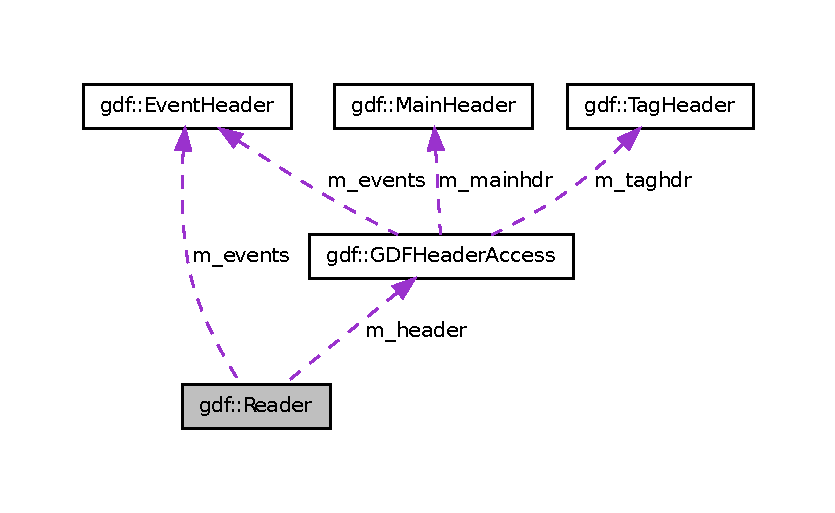
\includegraphics[width=400pt]{classgdf_1_1_reader__coll__graph}
\end{center}
\end{figure}
\subsection*{Public Member Functions}
\begin{DoxyCompactItemize}
\item 
\hypertarget{classgdf_1_1_reader_a0cfb8c260168d99aae5eecbfe6ddb23f}{
\hyperlink{classgdf_1_1_reader_a0cfb8c260168d99aae5eecbfe6ddb23f}{Reader} ()}
\label{classgdf_1_1_reader_a0cfb8c260168d99aae5eecbfe6ddb23f}

\begin{DoxyCompactList}\small\item\em Constructor. \item\end{DoxyCompactList}\item 
\hypertarget{classgdf_1_1_reader_a7a30b000e44df279c4524d134b7f5a9c}{
virtual \hyperlink{classgdf_1_1_reader_a7a30b000e44df279c4524d134b7f5a9c}{$\sim$Reader} ()}
\label{classgdf_1_1_reader_a7a30b000e44df279c4524d134b7f5a9c}

\begin{DoxyCompactList}\small\item\em Destructor. \item\end{DoxyCompactList}\item 
\hypertarget{classgdf_1_1_reader_ab0a373e03f5e30bbd727f4d89808fa46}{
void \hyperlink{classgdf_1_1_reader_ab0a373e03f5e30bbd727f4d89808fa46}{open} (const std::string filename)}
\label{classgdf_1_1_reader_ab0a373e03f5e30bbd727f4d89808fa46}

\begin{DoxyCompactList}\small\item\em Opens file for reading. \item\end{DoxyCompactList}\item 
\hypertarget{classgdf_1_1_reader_a9403aed29a6df769dc909025f8231bc8}{
void \hyperlink{classgdf_1_1_reader_a9403aed29a6df769dc909025f8231bc8}{close} ()}
\label{classgdf_1_1_reader_a9403aed29a6df769dc909025f8231bc8}

\begin{DoxyCompactList}\small\item\em Close file. \item\end{DoxyCompactList}\item 
\hypertarget{classgdf_1_1_reader_af409e126981ab1a0c5d106ec49d09179}{
void \hyperlink{classgdf_1_1_reader_af409e126981ab1a0c5d106ec49d09179}{enableCache} (bool b)}
\label{classgdf_1_1_reader_af409e126981ab1a0c5d106ec49d09179}

\begin{DoxyCompactList}\small\item\em Enable or disable cache. \item\end{DoxyCompactList}\item 
\hypertarget{classgdf_1_1_reader_ac27a7669548fce17720b2f9c61dcfc05}{
virtual void \hyperlink{classgdf_1_1_reader_ac27a7669548fce17720b2f9c61dcfc05}{resetCache} ()}
\label{classgdf_1_1_reader_ac27a7669548fce17720b2f9c61dcfc05}

\begin{DoxyCompactList}\small\item\em Reset cache to empty state. \item\end{DoxyCompactList}\item 
\hypertarget{classgdf_1_1_reader_a9178f346903ee5f9b47932f7208e7dfa}{
size\_\-t \hyperlink{classgdf_1_1_reader_a9178f346903ee5f9b47932f7208e7dfa}{findRecord} (uint16 channel\_\-idx, size\_\-t sample\_\-idx)}
\label{classgdf_1_1_reader_a9178f346903ee5f9b47932f7208e7dfa}

\begin{DoxyCompactList}\small\item\em Find \hyperlink{classgdf_1_1_record}{Record} index to which a sample belongs. \item\end{DoxyCompactList}\item 
void \hyperlink{classgdf_1_1_reader_ad1b1edc464cfe23b54c9ffc278677087}{getSignals} (std::vector$<$ std::vector$<$ double $>$ $>$ \&buffer, double start\_\-time=0, double end\_\-time=-\/1, std::vector$<$ uint16 $>$ signal\_\-indices=std::vector$<$ uint16 $>$())
\begin{DoxyCompactList}\small\item\em Read Signals from file into buffer (physical units). \item\end{DoxyCompactList}\item 
void \hyperlink{classgdf_1_1_reader_a2ad79c0649034f6462052ba088850c97}{getSignal} (uint16 channel\_\-idx, double $\ast$buffer, size\_\-t start=0, size\_\-t end=0)
\begin{DoxyCompactList}\small\item\em Read a single channel from file into buffer. \item\end{DoxyCompactList}\item 
double \hyperlink{classgdf_1_1_reader_ab0c56ba1256f76ac62663bd634fac79f}{getSample} (uint16 channel\_\-idx, size\_\-t sample\_\-idx)
\begin{DoxyCompactList}\small\item\em Read a single Sample (physical units). \item\end{DoxyCompactList}\item 
\hypertarget{classgdf_1_1_reader_aa0e1f6e08f7eee1627f0c42b05210649}{
\hyperlink{classgdf_1_1_record}{Record} $\ast$ \hyperlink{classgdf_1_1_reader_aa0e1f6e08f7eee1627f0c42b05210649}{getRecordPtr} (size\_\-t index)}
\label{classgdf_1_1_reader_aa0e1f6e08f7eee1627f0c42b05210649}

\begin{DoxyCompactList}\small\item\em Returns a reference to \hyperlink{classgdf_1_1_record}{Record}. \item\end{DoxyCompactList}\item 
\hypertarget{classgdf_1_1_reader_ae54fe50c79b21ec12bdc314164ccbc21}{
void \hyperlink{classgdf_1_1_reader_ae54fe50c79b21ec12bdc314164ccbc21}{precacheRecords} (size\_\-t start, size\_\-t end)}
\label{classgdf_1_1_reader_ae54fe50c79b21ec12bdc314164ccbc21}

\begin{DoxyCompactList}\small\item\em Precache a range of Records. \item\end{DoxyCompactList}\item 
\hypertarget{classgdf_1_1_reader_af10117d1c54e0aaa860e7f158cc7db15}{
\hyperlink{classgdf_1_1_event_header}{EventHeader} $\ast$ \hyperlink{classgdf_1_1_reader_af10117d1c54e0aaa860e7f158cc7db15}{getEventHeader} ()}
\label{classgdf_1_1_reader_af10117d1c54e0aaa860e7f158cc7db15}

\begin{DoxyCompactList}\small\item\em get reference to event header \item\end{DoxyCompactList}\end{DoxyCompactItemize}
\subsection*{Protected Member Functions}
\begin{DoxyCompactItemize}
\item 
\hypertarget{classgdf_1_1_reader_a300e99e98eb147c660edddf109a40116}{
void {\bfseries readEvents} ()}
\label{classgdf_1_1_reader_a300e99e98eb147c660edddf109a40116}

\end{DoxyCompactItemize}
\subsection*{Protected Attributes}
\begin{DoxyCompactItemize}
\item 
\hypertarget{classgdf_1_1_reader_a1cbc1a56b834026470b2c58b8ace18da}{
std::string {\bfseries m\_\-filename}}
\label{classgdf_1_1_reader_a1cbc1a56b834026470b2c58b8ace18da}

\item 
\hypertarget{classgdf_1_1_reader_a074adb287bd8f4f2c78eadac4003ef70}{
\hyperlink{classgdf_1_1_g_d_f_header_access}{GDFHeaderAccess} {\bfseries m\_\-header}}
\label{classgdf_1_1_reader_a074adb287bd8f4f2c78eadac4003ef70}

\item 
\hypertarget{classgdf_1_1_reader_a404e8fe0871d638a4082ea3e3d304849}{
\hyperlink{classgdf_1_1_event_header}{EventHeader} $\ast$ {\bfseries m\_\-events}}
\label{classgdf_1_1_reader_a404e8fe0871d638a4082ea3e3d304849}

\item 
\hypertarget{classgdf_1_1_reader_a98f8657c10545dbf96aa8815de772d91}{
std::vector$<$ boost::shared\_\-ptr$<$ \hyperlink{classgdf_1_1_record}{Record} $>$ $>$ {\bfseries m\_\-record\_\-cache}}
\label{classgdf_1_1_reader_a98f8657c10545dbf96aa8815de772d91}

\item 
\hypertarget{classgdf_1_1_reader_a393cf77dab3a8ede289da24fdb310372}{
std::ifstream {\bfseries m\_\-file}}
\label{classgdf_1_1_reader_a393cf77dab3a8ede289da24fdb310372}

\item 
\hypertarget{classgdf_1_1_reader_ad77fae214888cd06b33e8b487a990d0f}{
bool {\bfseries m\_\-cache\_\-enabled}}
\label{classgdf_1_1_reader_ad77fae214888cd06b33e8b487a990d0f}

\item 
\hypertarget{classgdf_1_1_reader_a5a0980f98d8e438da98594dc4a7c06c8}{
size\_\-t {\bfseries m\_\-record\_\-length}}
\label{classgdf_1_1_reader_a5a0980f98d8e438da98594dc4a7c06c8}

\item 
\hypertarget{classgdf_1_1_reader_a57f8b15044b4f5f396291e648dd48160}{
size\_\-t \hyperlink{classgdf_1_1_reader_a57f8b15044b4f5f396291e648dd48160}{m\_\-record\_\-offset}}
\label{classgdf_1_1_reader_a57f8b15044b4f5f396291e648dd48160}

\begin{DoxyCompactList}\small\item\em \hyperlink{classgdf_1_1_record}{Record} length in bytes. \item\end{DoxyCompactList}\item 
\hypertarget{classgdf_1_1_reader_a6cd9deb54aa60d60cdd3f99a9d090960}{
size\_\-t \hyperlink{classgdf_1_1_reader_a6cd9deb54aa60d60cdd3f99a9d090960}{m\_\-event\_\-offset}}
\label{classgdf_1_1_reader_a6cd9deb54aa60d60cdd3f99a9d090960}

\begin{DoxyCompactList}\small\item\em Where data records start in the file. \item\end{DoxyCompactList}\end{DoxyCompactItemize}


\subsection{Detailed Description}
Class for reading GDF files to disc. Data Records are only read on demand and stay in memory until another file is opened or the \hyperlink{classgdf_1_1_reader}{Reader} object is destroyed. This cache can be disabled. Then each data record is loaded from disk everytime it is accessed. This saves memory, but may severly decrease performance. 

\subsection{Member Function Documentation}
\hypertarget{classgdf_1_1_reader_ab0c56ba1256f76ac62663bd634fac79f}{
\index{gdf::Reader@{gdf::Reader}!getSample@{getSample}}
\index{getSample@{getSample}!gdf::Reader@{gdf::Reader}}
\subsubsection[{getSample}]{\setlength{\rightskip}{0pt plus 5cm}double gdf::Reader::getSample (
\begin{DoxyParamCaption}
\item[{uint16}]{ channel\_\-idx, }
\item[{size\_\-t}]{ sample\_\-idx}
\end{DoxyParamCaption}
)}}
\label{classgdf_1_1_reader_ab0c56ba1256f76ac62663bd634fac79f}


Read a single Sample (physical units). 


\begin{DoxyParams}{Parameters}
\item[\mbox{\tt[in]} {\em channel\_\-idx}]channel index \item[\mbox{\tt[in]} {\em sample\_\-idx}]sample index \end{DoxyParams}


Reimplemented in \hyperlink{classgdf_1_1_modifier_aa5d1ba80d46c3cd55f3930b586e57585}{gdf::Modifier}.



Here is the call graph for this function:
\nopagebreak
\begin{figure}[H]
\begin{center}
\leavevmode
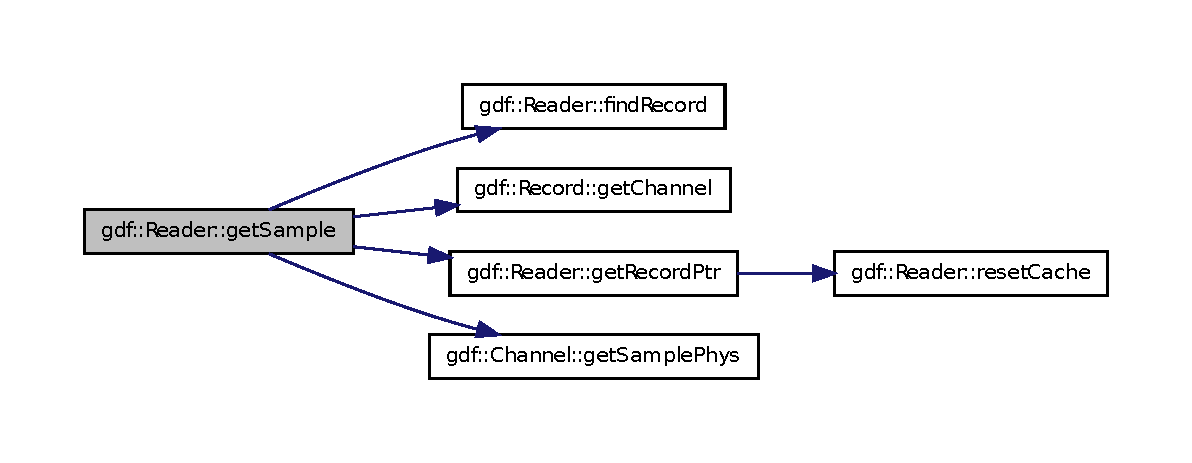
\includegraphics[width=400pt]{classgdf_1_1_reader_ab0c56ba1256f76ac62663bd634fac79f_cgraph}
\end{center}
\end{figure}


\hypertarget{classgdf_1_1_reader_a2ad79c0649034f6462052ba088850c97}{
\index{gdf::Reader@{gdf::Reader}!getSignal@{getSignal}}
\index{getSignal@{getSignal}!gdf::Reader@{gdf::Reader}}
\subsubsection[{getSignal}]{\setlength{\rightskip}{0pt plus 5cm}void gdf::Reader::getSignal (
\begin{DoxyParamCaption}
\item[{uint16}]{ channel\_\-idx, }
\item[{double $\ast$}]{ buffer, }
\item[{size\_\-t}]{ start = {\ttfamily 0}, }
\item[{size\_\-t}]{ end = {\ttfamily 0}}
\end{DoxyParamCaption}
)}}
\label{classgdf_1_1_reader_a2ad79c0649034f6462052ba088850c97}


Read a single channel from file into buffer. 

The buffer must be allocated by the user, who is also responsible that enough memory is allocated. 
\begin{DoxyParams}{Parameters}
\item[\mbox{\tt[in]} {\em channel\_\-idx}]index of channel to read \item[\mbox{\tt[out]} {\em buffer}]pointer to double array \item[\mbox{\tt[in]} {\em start\_\-time}]samples with n $>$= start are loaded. \item[\mbox{\tt[in]} {\em end\_\-time}]samples with n $<$ end are loaded. end $<$= start loads the complete signal. \end{DoxyParams}


Here is the call graph for this function:
\nopagebreak
\begin{figure}[H]
\begin{center}
\leavevmode
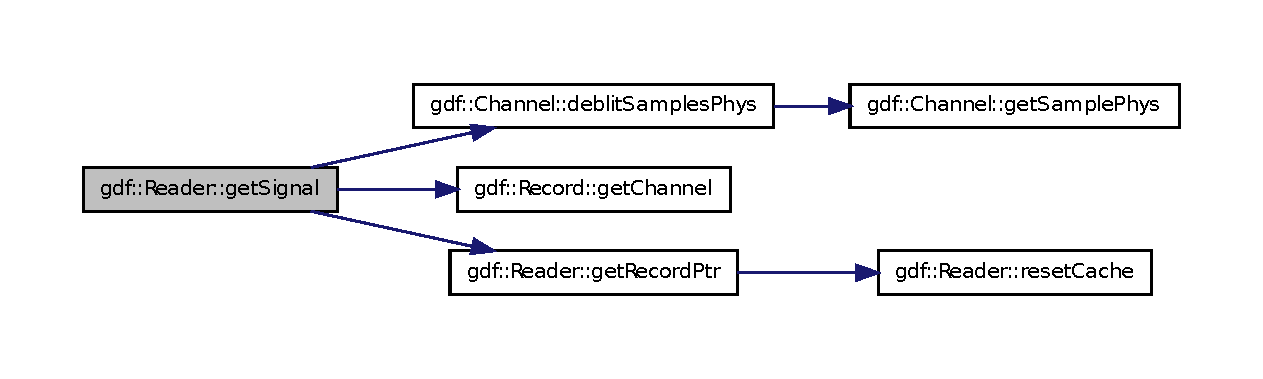
\includegraphics[width=400pt]{classgdf_1_1_reader_a2ad79c0649034f6462052ba088850c97_cgraph}
\end{center}
\end{figure}


\hypertarget{classgdf_1_1_reader_ad1b1edc464cfe23b54c9ffc278677087}{
\index{gdf::Reader@{gdf::Reader}!getSignals@{getSignals}}
\index{getSignals@{getSignals}!gdf::Reader@{gdf::Reader}}
\subsubsection[{getSignals}]{\setlength{\rightskip}{0pt plus 5cm}void gdf::Reader::getSignals (
\begin{DoxyParamCaption}
\item[{std::vector$<$ std::vector$<$ double $>$ $>$ \&}]{ buffer, }
\item[{double}]{ start\_\-time = {\ttfamily 0}, }
\item[{double}]{ end\_\-time = {\ttfamily -\/1}, }
\item[{std::vector$<$ uint16 $>$}]{ signal\_\-indices = {\ttfamily std::vector$<$uint16$>$()}}
\end{DoxyParamCaption}
)}}
\label{classgdf_1_1_reader_ad1b1edc464cfe23b54c9ffc278677087}


Read Signals from file into buffer (physical units). 

Sample values are converted to physical units. 
\begin{DoxyParams}{Parameters}
\item[\mbox{\tt[out]} {\em buffer}]vector; each element is a channel. \item[\mbox{\tt[in]} {\em start\_\-time}]samples with n $>$= start\_\-time$\ast$fs are loaded. \item[\mbox{\tt[in]} {\em end\_\-time}]samples with n $<$ end\_\-time$\ast$fs are loaded. end\_\-time = -\/1 loads the complete signal. \item[\mbox{\tt[in]} {\em signal\_\-indices}]vector with signal indices that should be loaded. If empty, all signals are loaded. \end{DoxyParams}


Here is the call graph for this function:
\nopagebreak
\begin{figure}[H]
\begin{center}
\leavevmode
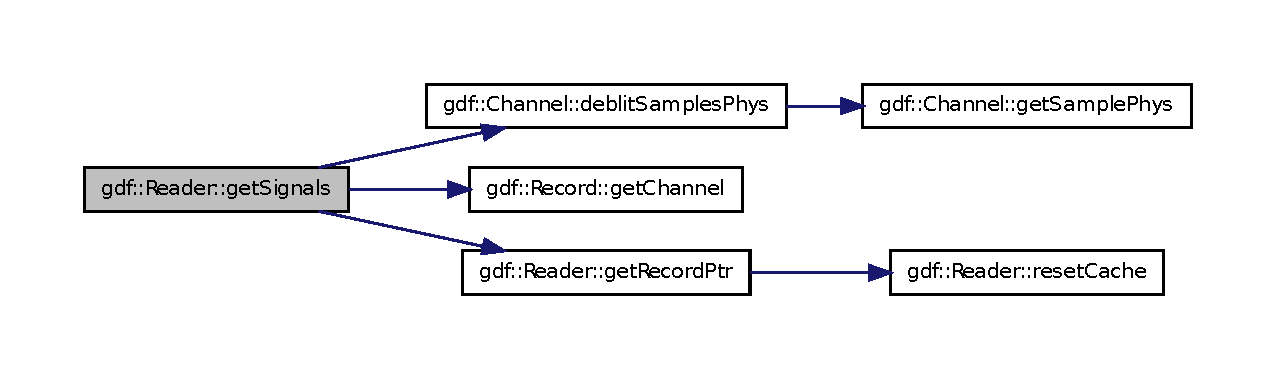
\includegraphics[width=400pt]{classgdf_1_1_reader_ad1b1edc464cfe23b54c9ffc278677087_cgraph}
\end{center}
\end{figure}




The documentation for this class was generated from the following files:\begin{DoxyCompactItemize}
\item 
include/GDF/Reader.h\item 
src/Reader.cpp\end{DoxyCompactItemize}

\hypertarget{classgdf_1_1_record}{
\section{gdf::Record Class Reference}
\label{classgdf_1_1_record}\index{gdf::Record@{gdf::Record}}
}


A \hyperlink{classgdf_1_1_record}{Record} is a block of data that contains a short time period of samples from all channels.  




{\ttfamily \#include $<$Record.h$>$}

\subsection*{Public Member Functions}
\begin{DoxyCompactItemize}
\item 
\hypertarget{classgdf_1_1_record_a708b6ae308bd5ebcf926fb0b78ea5242}{
\hyperlink{classgdf_1_1_record_a708b6ae308bd5ebcf926fb0b78ea5242}{Record} (const \hyperlink{classgdf_1_1_g_d_f_header_access}{GDFHeaderAccess} $\ast$hdr)}
\label{classgdf_1_1_record_a708b6ae308bd5ebcf926fb0b78ea5242}

\begin{DoxyCompactList}\small\item\em Constructor. \item\end{DoxyCompactList}\item 
\hypertarget{classgdf_1_1_record_a75d06616e1835c005bacd36451d7c23a}{
virtual \hyperlink{classgdf_1_1_record_a75d06616e1835c005bacd36451d7c23a}{$\sim$Record} ()}
\label{classgdf_1_1_record_a75d06616e1835c005bacd36451d7c23a}

\begin{DoxyCompactList}\small\item\em Destructor. \item\end{DoxyCompactList}\item 
void \hyperlink{classgdf_1_1_record_ae3a20e7fb29218efb793a8440688bfa6}{fill} ()
\begin{DoxyCompactList}\small\item\em Fills free samples in all channels with defined values. \item\end{DoxyCompactList}\item 
\hypertarget{classgdf_1_1_record_af5575c0f504c59507bb8e4d472edf5a7}{
bool \hyperlink{classgdf_1_1_record_af5575c0f504c59507bb8e4d472edf5a7}{isFull} () const }
\label{classgdf_1_1_record_af5575c0f504c59507bb8e4d472edf5a7}

\begin{DoxyCompactList}\small\item\em Returns true if all channels in the record have no free samples. \item\end{DoxyCompactList}\item 
\hypertarget{classgdf_1_1_record_ab75b4fa725bcdfddd08c4b3371ed48bd}{
bool \hyperlink{classgdf_1_1_record_ab75b4fa725bcdfddd08c4b3371ed48bd}{isEmpty} () const }
\label{classgdf_1_1_record_ab75b4fa725bcdfddd08c4b3371ed48bd}

\begin{DoxyCompactList}\small\item\em Returns true if all channels in the record are empty. \item\end{DoxyCompactList}\item 
\hypertarget{classgdf_1_1_record_a0d3b34f0085e5b1291ce0716f0f15f7d}{
\hyperlink{classgdf_1_1_channel}{Channel} $\ast$ \hyperlink{classgdf_1_1_record_a0d3b34f0085e5b1291ce0716f0f15f7d}{getChannel} (const size\_\-t chan\_\-idx)}
\label{classgdf_1_1_record_a0d3b34f0085e5b1291ce0716f0f15f7d}

\begin{DoxyCompactList}\small\item\em Returns reference to channel chan\_\-idx. \item\end{DoxyCompactList}\end{DoxyCompactItemize}
\subsection*{Friends}
\begin{DoxyCompactItemize}
\item 
\hypertarget{classgdf_1_1_record_abb5ecbb642f6c8c5fc28578757397e5f}{
std::ostream \& \hyperlink{classgdf_1_1_record_abb5ecbb642f6c8c5fc28578757397e5f}{operator$<$$<$} (std::ostream \&out, const \hyperlink{classgdf_1_1_record}{Record} \&c)}
\label{classgdf_1_1_record_abb5ecbb642f6c8c5fc28578757397e5f}

\begin{DoxyCompactList}\small\item\em \hyperlink{classgdf_1_1_record}{Record} Serializer. \item\end{DoxyCompactList}\item 
\hypertarget{classgdf_1_1_record_a8fe36dc766ee2beec048171871cf879e}{
std::istream \& \hyperlink{classgdf_1_1_record_a8fe36dc766ee2beec048171871cf879e}{operator$>$$>$} (std::istream \&in, \hyperlink{classgdf_1_1_record}{Record} \&c)}
\label{classgdf_1_1_record_a8fe36dc766ee2beec048171871cf879e}

\begin{DoxyCompactList}\small\item\em \hyperlink{classgdf_1_1_record}{Record} Deserializer. \item\end{DoxyCompactList}\end{DoxyCompactItemize}


\subsection{Detailed Description}
A \hyperlink{classgdf_1_1_record}{Record} is a block of data that contains a short time period of samples from all channels. 

\subsection{Member Function Documentation}
\hypertarget{classgdf_1_1_record_ae3a20e7fb29218efb793a8440688bfa6}{
\index{gdf::Record@{gdf::Record}!fill@{fill}}
\index{fill@{fill}!gdf::Record@{gdf::Record}}
\subsubsection[{fill}]{\setlength{\rightskip}{0pt plus 5cm}void gdf::Record::fill (
\begin{DoxyParamCaption}
{}
\end{DoxyParamCaption}
)}}
\label{classgdf_1_1_record_ae3a20e7fb29218efb793a8440688bfa6}


Fills free samples in all channels with defined values. 

This function is used to fill unfinished records before writing them to disc. For now we fill with NaNs if supported by the channel's data type and (physical) 0 otherwise. \begin{Desc}
\item[\hyperlink{todo__todo000001}{Todo}]What values should we fill in? NaN would be nice for floating point, but what about other data types? \end{Desc}


The documentation for this class was generated from the following files:\begin{DoxyCompactItemize}
\item 
include/GDF/Record.h\item 
src/Record.cpp\end{DoxyCompactItemize}

\hypertarget{classgdf_1_1_record_buffer}{
\section{gdf::RecordBuffer Class Reference}
\label{classgdf_1_1_record_buffer}\index{gdf::RecordBuffer@{gdf::RecordBuffer}}
}


Buffers incomplete records before they are written to disk.  




{\ttfamily \#include $<$RecordBuffer.h$>$}



Collaboration diagram for gdf::RecordBuffer:
\nopagebreak
\begin{figure}[H]
\begin{center}
\leavevmode
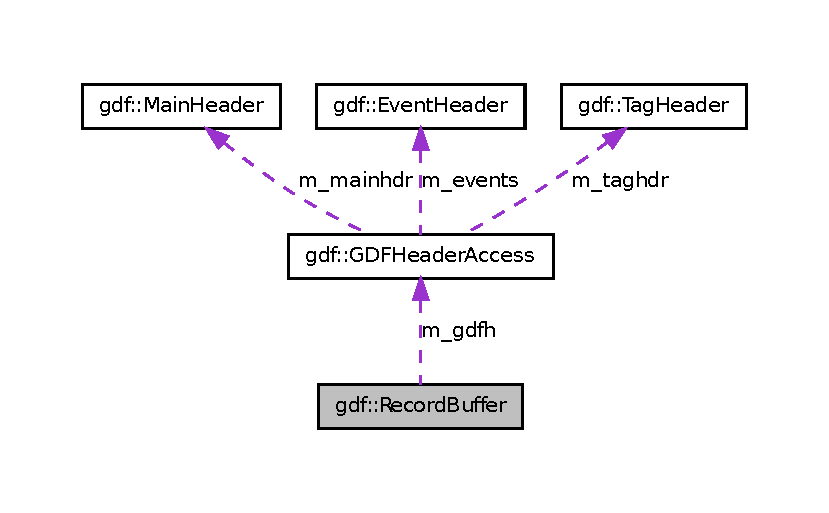
\includegraphics[width=398pt]{classgdf_1_1_record_buffer__coll__graph}
\end{center}
\end{figure}
\subsection*{Classes}
\begin{DoxyCompactItemize}
\item 
class \hyperlink{classgdf_1_1_record_buffer_1_1_record_full_handler}{RecordFullHandler}
\end{DoxyCompactItemize}
\subsection*{Public Member Functions}
\begin{DoxyCompactItemize}
\item 
\hypertarget{classgdf_1_1_record_buffer_a81a19745e41216424816d6f5d99d44a3}{
\hyperlink{classgdf_1_1_record_buffer_a81a19745e41216424816d6f5d99d44a3}{RecordBuffer} (const \hyperlink{classgdf_1_1_g_d_f_header_access}{GDFHeaderAccess} $\ast$gdfh)}
\label{classgdf_1_1_record_buffer_a81a19745e41216424816d6f5d99d44a3}

\begin{DoxyCompactList}\small\item\em Constructor. \item\end{DoxyCompactList}\item 
\hypertarget{classgdf_1_1_record_buffer_a4a1ead77698c8ffa21348609f96cac9a}{
virtual \hyperlink{classgdf_1_1_record_buffer_a4a1ead77698c8ffa21348609f96cac9a}{$\sim$RecordBuffer} ()}
\label{classgdf_1_1_record_buffer_a4a1ead77698c8ffa21348609f96cac9a}

\begin{DoxyCompactList}\small\item\em Destructor. \item\end{DoxyCompactList}\item 
\hypertarget{classgdf_1_1_record_buffer_a17d98ebe6d1c41ec7d367e59291697f9}{
void \hyperlink{classgdf_1_1_record_buffer_a17d98ebe6d1c41ec7d367e59291697f9}{reset} ()}
\label{classgdf_1_1_record_buffer_a17d98ebe6d1c41ec7d367e59291697f9}

\begin{DoxyCompactList}\small\item\em Resets the buffer to a valid initial state. \item\end{DoxyCompactList}\item 
void \hyperlink{classgdf_1_1_record_buffer_a7bd44e545daf03030de6e87a7903635a}{handleChannelFull} (const size\_\-t channel\_\-idx)
\begin{DoxyCompactList}\small\item\em Called when a channel becomes full. \item\end{DoxyCompactList}\item 
void \hyperlink{classgdf_1_1_record_buffer_a1ae270e60f9d483a06fe92df0cd664e4}{handleRecordFull} ()
\begin{DoxyCompactList}\small\item\em Called when a record becomes full. \item\end{DoxyCompactList}\item 
\hypertarget{classgdf_1_1_record_buffer_a9de2ad0f9c9020248d52d3ae64137489}{
void \hyperlink{classgdf_1_1_record_buffer_a9de2ad0f9c9020248d52d3ae64137489}{registerRecordFullCallback} (\hyperlink{classgdf_1_1_record_buffer_1_1_record_full_handler}{RecordFullHandler} $\ast$h)}
\label{classgdf_1_1_record_buffer_a9de2ad0f9c9020248d52d3ae64137489}

\begin{DoxyCompactList}\small\item\em Register Callback for record full event. \item\end{DoxyCompactList}\item 
\hypertarget{classgdf_1_1_record_buffer_a818a3b72f625ef7b0dc8bf8a79336bdf}{
void \hyperlink{classgdf_1_1_record_buffer_a818a3b72f625ef7b0dc8bf8a79336bdf}{unregisterRecordFullCallback} (\hyperlink{classgdf_1_1_record_buffer_1_1_record_full_handler}{RecordFullHandler} $\ast$h)}
\label{classgdf_1_1_record_buffer_a818a3b72f625ef7b0dc8bf8a79336bdf}

\begin{DoxyCompactList}\small\item\em Unegister Callback for record full event. \item\end{DoxyCompactList}\item 
\hypertarget{classgdf_1_1_record_buffer_ac516aef638abed8539809c42b18fcc47}{
void \hyperlink{classgdf_1_1_record_buffer_ac516aef638abed8539809c42b18fcc47}{addSamplePhys} (const size\_\-t channel\_\-idx, const double value)}
\label{classgdf_1_1_record_buffer_ac516aef638abed8539809c42b18fcc47}

\begin{DoxyCompactList}\small\item\em Add a physical sample to the channel specified by channel\_\-idx. \item\end{DoxyCompactList}\item 
\hypertarget{classgdf_1_1_record_buffer_ac60eef93ea59ab0f159b57d23412ee0f}{
{\footnotesize template$<$typename T $>$ }\\void \hyperlink{classgdf_1_1_record_buffer_ac60eef93ea59ab0f159b57d23412ee0f}{addSampleRaw} (const size\_\-t channel\_\-idx, const T rawval)}
\label{classgdf_1_1_record_buffer_ac60eef93ea59ab0f159b57d23412ee0f}

\begin{DoxyCompactList}\small\item\em Add a raw sample to the channel specified by channel\_\-idx. \item\end{DoxyCompactList}\item 
\hypertarget{classgdf_1_1_record_buffer_ada2965511d8ec8aa18c19761284a8690}{
void \hyperlink{classgdf_1_1_record_buffer_ada2965511d8ec8aa18c19761284a8690}{blitSamplesPhys} (const size\_\-t channel\_\-idx, const double $\ast$values, size\_\-t num)}
\label{classgdf_1_1_record_buffer_ada2965511d8ec8aa18c19761284a8690}

\begin{DoxyCompactList}\small\item\em Blit a number of physical samples into channel specified by channel\_\-idx. \item\end{DoxyCompactList}\item 
\hypertarget{classgdf_1_1_record_buffer_a554260febe2dc7bc56bb07756eb4f939}{
{\footnotesize template$<$typename T $>$ }\\void \hyperlink{classgdf_1_1_record_buffer_a554260febe2dc7bc56bb07756eb4f939}{blitSamplesRaw} (const size\_\-t channel\_\-idx, const T $\ast$values, size\_\-t num)}
\label{classgdf_1_1_record_buffer_a554260febe2dc7bc56bb07756eb4f939}

\begin{DoxyCompactList}\small\item\em Blit a number of raw samples into channel specified by channel\_\-idx. \item\end{DoxyCompactList}\item 
\hypertarget{classgdf_1_1_record_buffer_a20c9d5f7a970779e191b1a0eb84b4386}{
void \hyperlink{classgdf_1_1_record_buffer_a20c9d5f7a970779e191b1a0eb84b4386}{fillPhys} (const size\_\-t channel\_\-idx, const double value, size\_\-t num)}
\label{classgdf_1_1_record_buffer_a20c9d5f7a970779e191b1a0eb84b4386}

\begin{DoxyCompactList}\small\item\em Fill a number of samples with the same physical value. \item\end{DoxyCompactList}\item 
\hypertarget{classgdf_1_1_record_buffer_a153e1eeac18b088a86bf913671e4879b}{
{\footnotesize template$<$typename T $>$ }\\void \hyperlink{classgdf_1_1_record_buffer_a153e1eeac18b088a86bf913671e4879b}{fillRaw} (const size\_\-t channel\_\-idx, const T value, size\_\-t num)}
\label{classgdf_1_1_record_buffer_a153e1eeac18b088a86bf913671e4879b}

\begin{DoxyCompactList}\small\item\em Fill a number of samples with the same raw value. \item\end{DoxyCompactList}\item 
void \hyperlink{classgdf_1_1_record_buffer_a97e676d68f9aa9441c301c78b46f0a4d}{addRecord} (\hyperlink{classgdf_1_1_record}{Record} \&r)
\begin{DoxyCompactList}\small\item\em Add a complete \hyperlink{classgdf_1_1_record}{Record}. \item\end{DoxyCompactList}\item 
\hypertarget{classgdf_1_1_record_buffer_a21f20828bffa27e1ed7383eacde6a927}{
std::list$<$ boost::shared\_\-ptr$<$ \hyperlink{classgdf_1_1_record}{Record} $>$ $>$::iterator \hyperlink{classgdf_1_1_record_buffer_a21f20828bffa27e1ed7383eacde6a927}{createNewRecord} ()}
\label{classgdf_1_1_record_buffer_a21f20828bffa27e1ed7383eacde6a927}

\begin{DoxyCompactList}\small\item\em Put a new record to the end of the list. \item\end{DoxyCompactList}\item 
\hypertarget{classgdf_1_1_record_buffer_ab4f141c5c15a7c92be005758ef8231e2}{
\hyperlink{classgdf_1_1_record}{Record} $\ast$ \hyperlink{classgdf_1_1_record_buffer_ab4f141c5c15a7c92be005758ef8231e2}{getFirstFullRecord} ()}
\label{classgdf_1_1_record_buffer_ab4f141c5c15a7c92be005758ef8231e2}

\begin{DoxyCompactList}\small\item\em Reference to first (oldest) full record in list. This is also the first record that gets filled. \item\end{DoxyCompactList}\item 
\hypertarget{classgdf_1_1_record_buffer_aea0c7b33b23e3f4d97cc2398d27e740b}{
void \hyperlink{classgdf_1_1_record_buffer_aea0c7b33b23e3f4d97cc2398d27e740b}{removeFirstFullRecord} ()}
\label{classgdf_1_1_record_buffer_aea0c7b33b23e3f4d97cc2398d27e740b}

\begin{DoxyCompactList}\small\item\em Remove first full record in list. \item\end{DoxyCompactList}\item 
\hypertarget{classgdf_1_1_record_buffer_a3573e58d036d703a5862d859e9f7395c}{
size\_\-t \hyperlink{classgdf_1_1_record_buffer_a3573e58d036d703a5862d859e9f7395c}{getNumFullRecords} ()}
\label{classgdf_1_1_record_buffer_a3573e58d036d703a5862d859e9f7395c}

\begin{DoxyCompactList}\small\item\em Get number of full records in the buffer. \item\end{DoxyCompactList}\item 
\hypertarget{classgdf_1_1_record_buffer_a26a79cdf41e61e9bf900b5c044e41777}{
size\_\-t \hyperlink{classgdf_1_1_record_buffer_a26a79cdf41e61e9bf900b5c044e41777}{getNumPartialRecords} ()}
\label{classgdf_1_1_record_buffer_a26a79cdf41e61e9bf900b5c044e41777}

\begin{DoxyCompactList}\small\item\em Get number of partially filled records currently in the list. \item\end{DoxyCompactList}\item 
\hyperlink{classgdf_1_1_channel}{Channel} $\ast$ \hyperlink{classgdf_1_1_record_buffer_a780d3156d97dd0e2f7121e813419035a}{getValidChannel} (const size\_\-t channel\_\-idx)
\begin{DoxyCompactList}\small\item\em Returns reference to channel specified by channel\_\-idx. \item\end{DoxyCompactList}\item 
\hypertarget{classgdf_1_1_record_buffer_a924508d9e9988f4a97545b3070a2d156}{
size\_\-t \hyperlink{classgdf_1_1_record_buffer_a924508d9e9988f4a97545b3070a2d156}{getNumFreeAlloc} (const size\_\-t channel\_\-idx)}
\label{classgdf_1_1_record_buffer_a924508d9e9988f4a97545b3070a2d156}

\begin{DoxyCompactList}\small\item\em Gets number of free samples currently allocated for this channel. \item\end{DoxyCompactList}\item 
\hypertarget{classgdf_1_1_record_buffer_ad58cb7b3c52b576d35abab83db4b5cad}{
void \hyperlink{classgdf_1_1_record_buffer_ad58cb7b3c52b576d35abab83db4b5cad}{flood} ()}
\label{classgdf_1_1_record_buffer_ad58cb7b3c52b576d35abab83db4b5cad}

\begin{DoxyCompactList}\small\item\em Fills all partial records with default values. \item\end{DoxyCompactList}\end{DoxyCompactItemize}


\subsection{Detailed Description}
Buffers incomplete records before they are written to disk. When saving data, one or more channels can be ahead of the others, and may even extend over multiple records. \hyperlink{classgdf_1_1_record_buffer}{RecordBuffer} takes care of this by creating a new record as soon a channel exceeds it's capacity. 

\subsection{Member Function Documentation}
\hypertarget{classgdf_1_1_record_buffer_a97e676d68f9aa9441c301c78b46f0a4d}{
\index{gdf::RecordBuffer@{gdf::RecordBuffer}!addRecord@{addRecord}}
\index{addRecord@{addRecord}!gdf::RecordBuffer@{gdf::RecordBuffer}}
\subsubsection[{addRecord}]{\setlength{\rightskip}{0pt plus 5cm}void gdf::RecordBuffer::addRecord (
\begin{DoxyParamCaption}
\item[{{\bf Record} \&}]{ r}
\end{DoxyParamCaption}
)}}
\label{classgdf_1_1_record_buffer_a97e676d68f9aa9441c301c78b46f0a4d}


Add a complete \hyperlink{classgdf_1_1_record}{Record}. 

There may not be any partial records in the buffer in order to add a complete record. 

Here is the call graph for this function:
\nopagebreak
\begin{figure}[H]
\begin{center}
\leavevmode
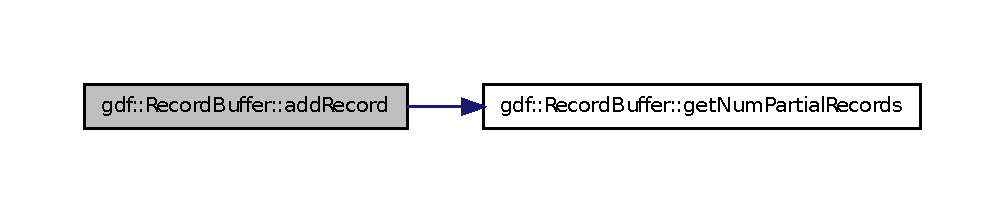
\includegraphics[width=400pt]{classgdf_1_1_record_buffer_a97e676d68f9aa9441c301c78b46f0a4d_cgraph}
\end{center}
\end{figure}




Here is the caller graph for this function:
\nopagebreak
\begin{figure}[H]
\begin{center}
\leavevmode
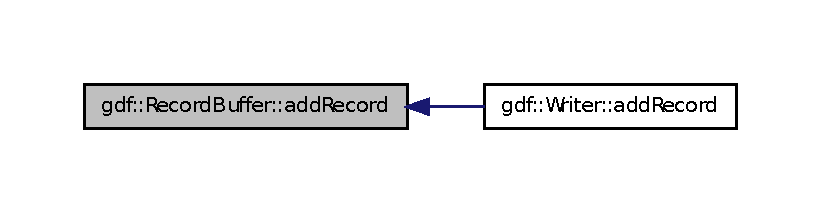
\includegraphics[width=394pt]{classgdf_1_1_record_buffer_a97e676d68f9aa9441c301c78b46f0a4d_icgraph}
\end{center}
\end{figure}


\hypertarget{classgdf_1_1_record_buffer_a780d3156d97dd0e2f7121e813419035a}{
\index{gdf::RecordBuffer@{gdf::RecordBuffer}!getValidChannel@{getValidChannel}}
\index{getValidChannel@{getValidChannel}!gdf::RecordBuffer@{gdf::RecordBuffer}}
\subsubsection[{getValidChannel}]{\setlength{\rightskip}{0pt plus 5cm}{\bf Channel} $\ast$ gdf::RecordBuffer::getValidChannel (
\begin{DoxyParamCaption}
\item[{const size\_\-t}]{ channel\_\-idx}
\end{DoxyParamCaption}
)}}
\label{classgdf_1_1_record_buffer_a780d3156d97dd0e2f7121e813419035a}


Returns reference to channel specified by channel\_\-idx. 

If channel does not exist gdf::nonexistent\_\-channel\_\-access::nonexistent\_\-channel\_\-access is thrown. A new record is created if the channelhead points to the end of the record list. 

Here is the call graph for this function:
\nopagebreak
\begin{figure}[H]
\begin{center}
\leavevmode
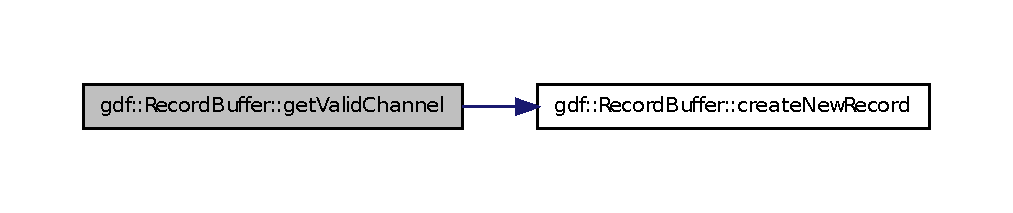
\includegraphics[width=400pt]{classgdf_1_1_record_buffer_a780d3156d97dd0e2f7121e813419035a_cgraph}
\end{center}
\end{figure}




Here is the caller graph for this function:
\nopagebreak
\begin{figure}[H]
\begin{center}
\leavevmode
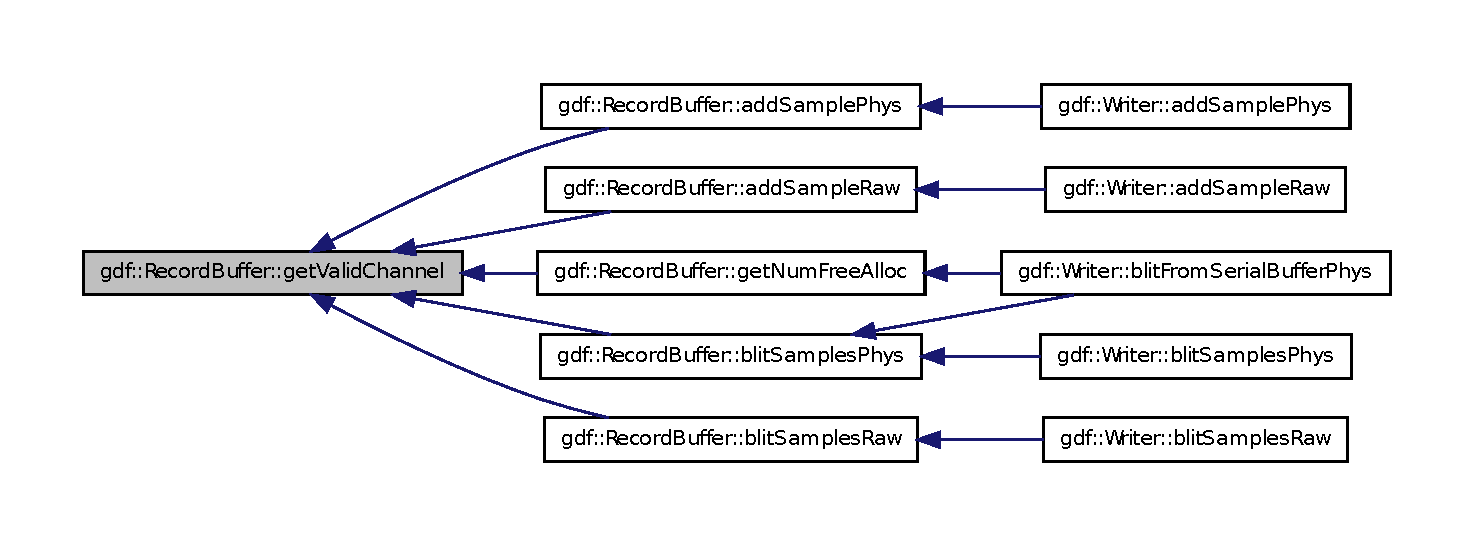
\includegraphics[width=400pt]{classgdf_1_1_record_buffer_a780d3156d97dd0e2f7121e813419035a_icgraph}
\end{center}
\end{figure}


\hypertarget{classgdf_1_1_record_buffer_a7bd44e545daf03030de6e87a7903635a}{
\index{gdf::RecordBuffer@{gdf::RecordBuffer}!handleChannelFull@{handleChannelFull}}
\index{handleChannelFull@{handleChannelFull}!gdf::RecordBuffer@{gdf::RecordBuffer}}
\subsubsection[{handleChannelFull}]{\setlength{\rightskip}{0pt plus 5cm}void gdf::RecordBuffer::handleChannelFull (
\begin{DoxyParamCaption}
\item[{const size\_\-t}]{ channel\_\-idx}
\end{DoxyParamCaption}
)}}
\label{classgdf_1_1_record_buffer_a7bd44e545daf03030de6e87a7903635a}


Called when a channel becomes full. 

This function advances the write pointer m\_\-channelhead for this channel to the next record. If there is no next record, a new one is created. Also checks if the current record is full and performs calls the respective handler. 

Here is the call graph for this function:
\nopagebreak
\begin{figure}[H]
\begin{center}
\leavevmode
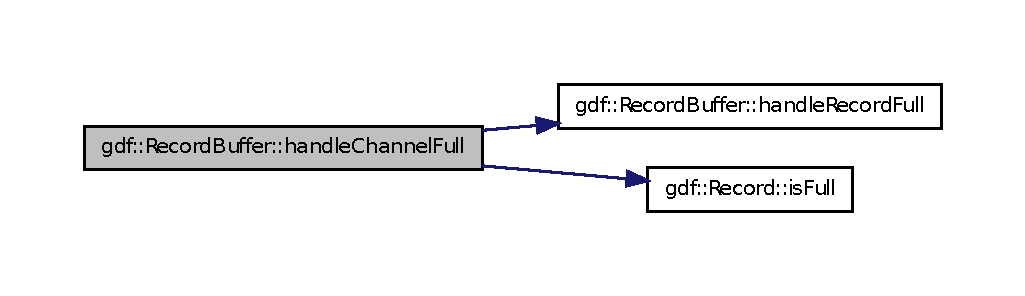
\includegraphics[width=400pt]{classgdf_1_1_record_buffer_a7bd44e545daf03030de6e87a7903635a_cgraph}
\end{center}
\end{figure}




Here is the caller graph for this function:
\nopagebreak
\begin{figure}[H]
\begin{center}
\leavevmode
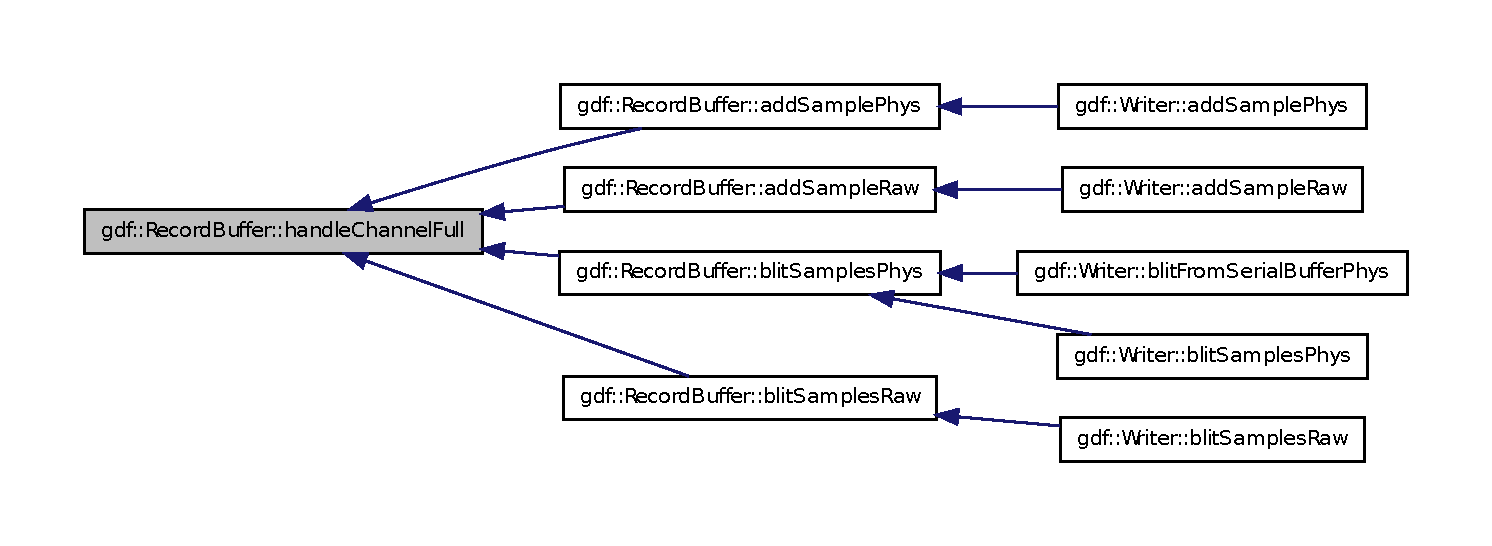
\includegraphics[width=400pt]{classgdf_1_1_record_buffer_a7bd44e545daf03030de6e87a7903635a_icgraph}
\end{center}
\end{figure}


\hypertarget{classgdf_1_1_record_buffer_a1ae270e60f9d483a06fe92df0cd664e4}{
\index{gdf::RecordBuffer@{gdf::RecordBuffer}!handleRecordFull@{handleRecordFull}}
\index{handleRecordFull@{handleRecordFull}!gdf::RecordBuffer@{gdf::RecordBuffer}}
\subsubsection[{handleRecordFull}]{\setlength{\rightskip}{0pt plus 5cm}void gdf::RecordBuffer::handleRecordFull (
\begin{DoxyParamCaption}
{}
\end{DoxyParamCaption}
)}}
\label{classgdf_1_1_record_buffer_a1ae270e60f9d483a06fe92df0cd664e4}


Called when a record becomes full. 



Here is the caller graph for this function:
\nopagebreak
\begin{figure}[H]
\begin{center}
\leavevmode
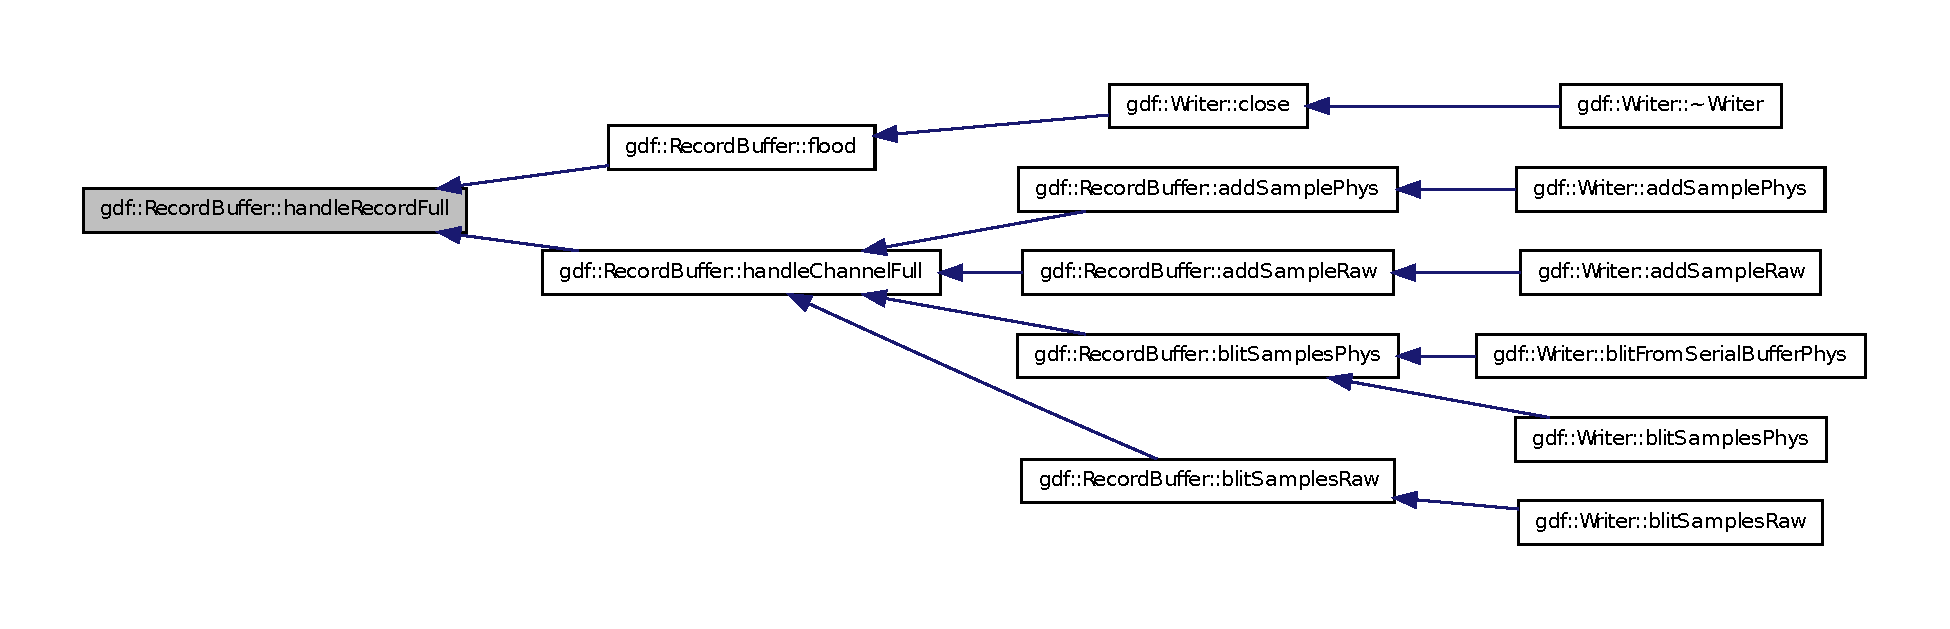
\includegraphics[width=400pt]{classgdf_1_1_record_buffer_a1ae270e60f9d483a06fe92df0cd664e4_icgraph}
\end{center}
\end{figure}




The documentation for this class was generated from the following files:\begin{DoxyCompactItemize}
\item 
include/GDF/RecordBuffer.h\item 
src/RecordBuffer.cpp\end{DoxyCompactItemize}

\hypertarget{classgdf_1_1_record_buffer_1_1_record_full_handler}{
\section{gdf::RecordBuffer::RecordFullHandler Class Reference}
\label{classgdf_1_1_record_buffer_1_1_record_full_handler}\index{gdf::RecordBuffer::RecordFullHandler@{gdf::RecordBuffer::RecordFullHandler}}
}


Inherited by \hyperlink{classgdf_1_1_writer}{gdf::Writer}.

\subsection*{Public Member Functions}
\begin{DoxyCompactItemize}
\item 
\hypertarget{classgdf_1_1_record_buffer_1_1_record_full_handler_adf2e9f871aed8926a66a8fa52d1694b7}{
virtual void {\bfseries triggerRecordFull} (\hyperlink{classgdf_1_1_record}{Record} $\ast$rec)=0}
\label{classgdf_1_1_record_buffer_1_1_record_full_handler_adf2e9f871aed8926a66a8fa52d1694b7}

\end{DoxyCompactItemize}


The documentation for this class was generated from the following file:\begin{DoxyCompactItemize}
\item 
include/GDF/RecordBuffer.h\end{DoxyCompactItemize}

\hypertarget{classgdf_1_1exception_1_1serialization__error}{
\section{gdf::exception::serialization\_\-error Class Reference}
\label{classgdf_1_1exception_1_1serialization__error}\index{gdf::exception::serialization\_\-error@{gdf::exception::serialization\_\-error}}
}


File exists.  




{\ttfamily \#include $<$Exceptions.h$>$}

\subsection*{Public Member Functions}
\begin{DoxyCompactItemize}
\item 
\hypertarget{classgdf_1_1exception_1_1serialization__error_aa9d45cd5cb4ec85d41295bfe0a32b161}{
{\bfseries serialization\_\-error} (std::string str)}
\label{classgdf_1_1exception_1_1serialization__error_aa9d45cd5cb4ec85d41295bfe0a32b161}

\end{DoxyCompactItemize}


\subsection{Detailed Description}
File exists. 

The documentation for this class was generated from the following file:\begin{DoxyCompactItemize}
\item 
include/GDF/Exceptions.h\end{DoxyCompactItemize}

\hypertarget{classgdf_1_1exception_1_1signal__exists}{
\section{gdf::exception::signal\_\-exists Class Reference}
\label{classgdf_1_1exception_1_1signal__exists}\index{gdf::exception::signal\_\-exists@{gdf::exception::signal\_\-exists}}
}


\hyperlink{classgdf_1_1_channel}{Channel} does exist.  




{\ttfamily \#include $<$Exceptions.h$>$}

\subsection*{Public Member Functions}
\begin{DoxyCompactItemize}
\item 
\hypertarget{classgdf_1_1exception_1_1signal__exists_a80bf174a9953309cddce10454d6abafb}{
{\bfseries signal\_\-exists} (std::string str)}
\label{classgdf_1_1exception_1_1signal__exists_a80bf174a9953309cddce10454d6abafb}

\end{DoxyCompactItemize}


\subsection{Detailed Description}
\hyperlink{classgdf_1_1_channel}{Channel} does exist. 

The documentation for this class was generated from the following file:\begin{DoxyCompactItemize}
\item 
include/GDF/Exceptions.h\end{DoxyCompactItemize}

\hypertarget{classgdf_1_1exception_1_1signal__exists__not}{
\section{gdf::exception::signal\_\-exists\_\-not Class Reference}
\label{classgdf_1_1exception_1_1signal__exists__not}\index{gdf::exception::signal\_\-exists\_\-not@{gdf::exception::signal\_\-exists\_\-not}}
}


\hyperlink{classgdf_1_1_channel}{Channel} does not exist.  




{\ttfamily \#include $<$Exceptions.h$>$}

\subsection*{Public Member Functions}
\begin{DoxyCompactItemize}
\item 
\hypertarget{classgdf_1_1exception_1_1signal__exists__not_a79235e74936b1ba16f85db1cd3539ab3}{
{\bfseries signal\_\-exists\_\-not} (std::string str)}
\label{classgdf_1_1exception_1_1signal__exists__not_a79235e74936b1ba16f85db1cd3539ab3}

\end{DoxyCompactItemize}


\subsection{Detailed Description}
\hyperlink{classgdf_1_1_channel}{Channel} does not exist. 

The documentation for this class was generated from the following file:\begin{DoxyCompactItemize}
\item 
include/GDF/Exceptions.h\end{DoxyCompactItemize}

\hypertarget{classgdf_1_1_signal_header}{
\section{gdf::SignalHeader Class Reference}
\label{classgdf_1_1_signal_header}\index{gdf::SignalHeader@{gdf::SignalHeader}}
}


Contains all information required to construct the GDF signal header.  




{\ttfamily \#include $<$SignalHeader.h$>$}

\subsection*{Friends}
\begin{DoxyCompactItemize}
\item 
\hypertarget{classgdf_1_1_signal_header_ade47bf1d3f5a91747dd7fbb489fbcab0}{
class {\bfseries GDFHeaderAccess}}
\label{classgdf_1_1_signal_header_ade47bf1d3f5a91747dd7fbb489fbcab0}

\item 
\hypertarget{classgdf_1_1_signal_header_a0dd6213f6ada6c22b9c2e8e7890305a2}{
std::ostream \& \hyperlink{classgdf_1_1_signal_header_a0dd6213f6ada6c22b9c2e8e7890305a2}{operator$<$$<$} (std::ostream \&out, const \hyperlink{classgdf_1_1_g_d_f_header_access}{GDFHeaderAccess} \&hdr)}
\label{classgdf_1_1_signal_header_a0dd6213f6ada6c22b9c2e8e7890305a2}

\begin{DoxyCompactList}\small\item\em Header Serializer. \item\end{DoxyCompactList}\item 
\hypertarget{classgdf_1_1_signal_header_a0a4dea8648fdd7b1131f900f772d2961}{
std::istream \& \hyperlink{classgdf_1_1_signal_header_a0a4dea8648fdd7b1131f900f772d2961}{operator$>$$>$} (std::istream \&in, \hyperlink{classgdf_1_1_g_d_f_header_access}{GDFHeaderAccess} \&hdr)}
\label{classgdf_1_1_signal_header_a0a4dea8648fdd7b1131f900f772d2961}

\begin{DoxyCompactList}\small\item\em Header Deserializer. \item\end{DoxyCompactList}\end{DoxyCompactItemize}


\subsection{Detailed Description}
Contains all information required to construct the GDF signal header. 

The documentation for this class was generated from the following files:\begin{DoxyCompactItemize}
\item 
include/GDF/SignalHeader.h\item 
src/SignalHeader.cpp\end{DoxyCompactItemize}

\hypertarget{classgdf_1_1_tag_header}{
\section{gdf::TagHeader Class Reference}
\label{classgdf_1_1_tag_header}\index{gdf::TagHeader@{gdf::TagHeader}}
}


Contains all information required to construct the optional GDF tag header.  




{\ttfamily \#include $<$TagHeader.h$>$}

\subsection*{Public Member Functions}
\begin{DoxyCompactItemize}
\item 
\hypertarget{classgdf_1_1_tag_header_a27ca1dab24ac2407af9071831876059b}{
size\_\-t \hyperlink{classgdf_1_1_tag_header_a27ca1dab24ac2407af9071831876059b}{getLength} ()}
\label{classgdf_1_1_tag_header_a27ca1dab24ac2407af9071831876059b}

\begin{DoxyCompactList}\small\item\em Returns number the length of the header (number of 256 byte blocks). \item\end{DoxyCompactList}\end{DoxyCompactItemize}


\subsection{Detailed Description}
Contains all information required to construct the optional GDF tag header. 

The documentation for this class was generated from the following file:\begin{DoxyCompactItemize}
\item 
include/GDF/TagHeader.h\end{DoxyCompactItemize}

\hypertarget{classgdf_1_1_writer}{
\section{gdf::Writer Class Reference}
\label{classgdf_1_1_writer}\index{gdf::Writer@{gdf::Writer}}
}


Class for writing GDF files to disc.  




{\ttfamily \#include $<$Writer.h$>$}



Inherits \hyperlink{classgdf_1_1_record_buffer_1_1_record_full_handler}{gdf::RecordBuffer::RecordFullHandler}.



Collaboration diagram for gdf::Writer:
\nopagebreak
\begin{figure}[H]
\begin{center}
\leavevmode
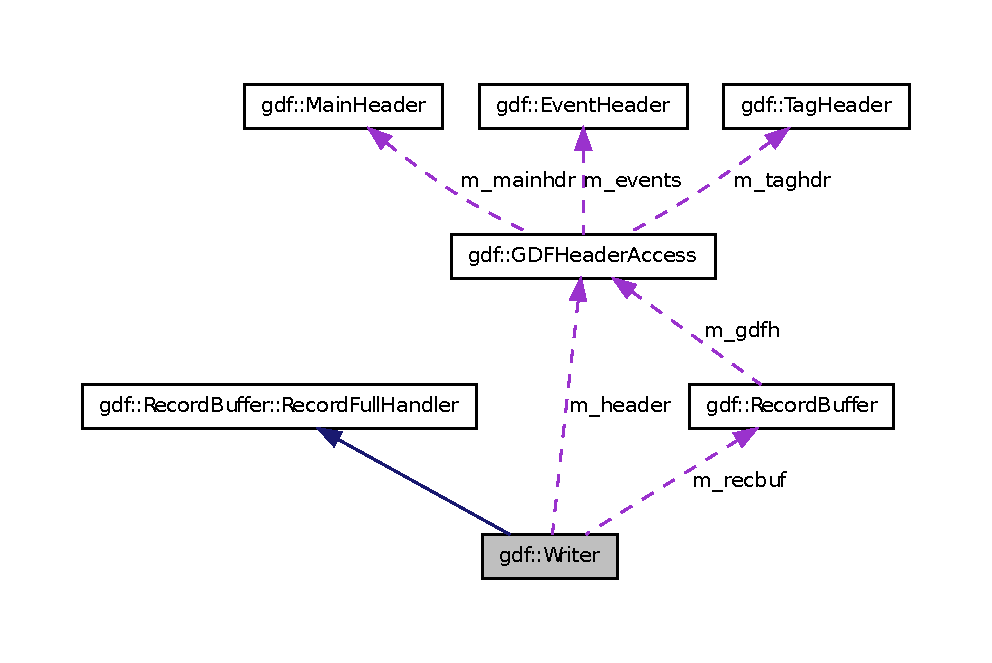
\includegraphics[width=400pt]{classgdf_1_1_writer__coll__graph}
\end{center}
\end{figure}
\subsection*{Public Member Functions}
\begin{DoxyCompactItemize}
\item 
\hypertarget{classgdf_1_1_writer_a612e93a7862d4fa9c871a7e62399048c}{
\hyperlink{classgdf_1_1_writer_a612e93a7862d4fa9c871a7e62399048c}{Writer} ()}
\label{classgdf_1_1_writer_a612e93a7862d4fa9c871a7e62399048c}

\begin{DoxyCompactList}\small\item\em Constructor. \item\end{DoxyCompactList}\item 
\hypertarget{classgdf_1_1_writer_a6a436f443584c4daa94a941e2f202dfc}{
virtual \hyperlink{classgdf_1_1_writer_a6a436f443584c4daa94a941e2f202dfc}{$\sim$Writer} ()}
\label{classgdf_1_1_writer_a6a436f443584c4daa94a941e2f202dfc}

\begin{DoxyCompactList}\small\item\em Destructor. \item\end{DoxyCompactList}\item 
void \hyperlink{classgdf_1_1_writer_a984bb670f2ca17c85916924877edab39}{open} (const int flags=writer\_\-ev\_\-file)
\begin{DoxyCompactList}\small\item\em Opens file for writing and writes Header. \item\end{DoxyCompactList}\item 
void \hyperlink{classgdf_1_1_writer_ab493c0c6beb99d11d0cba1a229681e44}{open} (const std::string filename, const int flags=writer\_\-ev\_\-file)
\begin{DoxyCompactList}\small\item\em Opens file for writing and writes Header. \item\end{DoxyCompactList}\item 
void \hyperlink{classgdf_1_1_writer_ae5856d4b6ca98e7af552d99d830433c9}{close} ()
\begin{DoxyCompactList}\small\item\em Close file. \item\end{DoxyCompactList}\item 
\hypertarget{classgdf_1_1_writer_abc4c99004fc2275bc25dddb95e164e10}{
bool \hyperlink{classgdf_1_1_writer_abc4c99004fc2275bc25dddb95e164e10}{isOpen} ()}
\label{classgdf_1_1_writer_abc4c99004fc2275bc25dddb95e164e10}

\begin{DoxyCompactList}\small\item\em Check if file is open. \item\end{DoxyCompactList}\item 
void \hyperlink{classgdf_1_1_writer_ad8cab49e3b866304802924707fd9d367}{setFilename} (std::string filename)
\begin{DoxyCompactList}\small\item\em set filename for later opening \item\end{DoxyCompactList}\item 
void \hyperlink{classgdf_1_1_writer_a15b2d4702b41521a1dba4fe8b7f2986a}{setMaxFullRecords} (size\_\-t num)
\begin{DoxyCompactList}\small\item\em Set number of full records that are kept in memory before the buffer is flushed. \item\end{DoxyCompactList}\item 
bool \hyperlink{classgdf_1_1_writer_ab0dc03f3e4f125695c40c09ce66d9d16}{createSignal} (size\_\-t index, bool throwexc=false)
\begin{DoxyCompactList}\small\item\em Create a signal. \item\end{DoxyCompactList}\item 
void \hyperlink{classgdf_1_1_writer_a25563ed9d61e7b6935dc09bc469c9eb7}{swapSignals} (size\_\-t a, size\_\-t b)
\begin{DoxyCompactList}\small\item\em Swap to signals. \item\end{DoxyCompactList}\item 
void \hyperlink{classgdf_1_1_writer_ab69e32b0fb120731544cbff10d6e3a3f}{relocateSignal} (size\_\-t src, size\_\-t dst)
\begin{DoxyCompactList}\small\item\em Change signal index. \item\end{DoxyCompactList}\item 
\hypertarget{classgdf_1_1_writer_ae7328f77c14354b57608c9c8097e4a51}{
size\_\-t \hyperlink{classgdf_1_1_writer_ae7328f77c14354b57608c9c8097e4a51}{getFirstFreeSignalIndex} ()}
\label{classgdf_1_1_writer_ae7328f77c14354b57608c9c8097e4a51}

\begin{DoxyCompactList}\small\item\em get lowest signal index that can be created \item\end{DoxyCompactList}\item 
void \hyperlink{classgdf_1_1_writer_a78c344714054c13d96e0c85af24ad19f}{blitFromSerialBufferPhys} (const double $\ast$buf, const std::vector$<$ size\_\-t $>$ \&samples\_\-per\_\-channel)
\begin{DoxyCompactList}\small\item\em Blit data from a serial buffer. \item\end{DoxyCompactList}\item 
void \hyperlink{classgdf_1_1_writer_aeb0e491af4de91e79469634d8b3ecc5d}{addSamplePhys} (const size\_\-t channel\_\-idx, const float64 value)
\begin{DoxyCompactList}\small\item\em Add sample in physical units to a channel. \item\end{DoxyCompactList}\item 
{\footnotesize template$<$typename T $>$ }\\void \hyperlink{classgdf_1_1_writer_a072237c5d82136be71668611a27111fc}{addSampleRaw} (const size\_\-t channel\_\-idx, const T value)
\begin{DoxyCompactList}\small\item\em Add a raw sample to channel. \item\end{DoxyCompactList}\item 
void \hyperlink{classgdf_1_1_writer_a3e01dfba57c77e5cac1db767de79b650}{blitSamplesPhys} (const size\_\-t channel\_\-idx, const float64 $\ast$values, size\_\-t num)
\begin{DoxyCompactList}\small\item\em Blit a number of samples in physical units to channel. \item\end{DoxyCompactList}\item 
void \hyperlink{classgdf_1_1_writer_af8b7e224467b9b706e4eaec7672d8399}{blitSamplesPhys} (const size\_\-t channel\_\-idx, const std::vector$<$ float64 $>$ \&values)
\begin{DoxyCompactList}\small\item\em Blit a number of samples in physical units to channel. \item\end{DoxyCompactList}\item 
{\footnotesize template$<$typename T $>$ }\\void \hyperlink{classgdf_1_1_writer_a2faf6a7c8aa18f81aadd0ff42eeb5caf}{blitSamplesRaw} (const size\_\-t channel\_\-idx, const T $\ast$values, size\_\-t num)
\begin{DoxyCompactList}\small\item\em Blit a number of raw samples to channel. \item\end{DoxyCompactList}\item 
{\footnotesize template$<$typename T $>$ }\\void \hyperlink{classgdf_1_1_writer_ae9eb09e9e7017fafaa6c367ec74d66bb}{blitSamplesRaw} (const size\_\-t channel\_\-idx, const std::vector$<$ T $>$ \&values)
\begin{DoxyCompactList}\small\item\em Blit a number of raw samples to channel. \item\end{DoxyCompactList}\item 
void \hyperlink{classgdf_1_1_writer_aa067a56c9699ad0c0a9fbebf83724dec}{addRecord} (\hyperlink{classgdf_1_1_record}{Record} \&r)
\begin{DoxyCompactList}\small\item\em Add a complete \hyperlink{classgdf_1_1_record}{Record}. \item\end{DoxyCompactList}\item 
\hypertarget{classgdf_1_1_writer_a14c39a92ac6f19312b2561363283d3e4}{
void \hyperlink{classgdf_1_1_writer_a14c39a92ac6f19312b2561363283d3e4}{flush} ()}
\label{classgdf_1_1_writer_a14c39a92ac6f19312b2561363283d3e4}

\begin{DoxyCompactList}\small\item\em writes all full records from buffer to disc \item\end{DoxyCompactList}\item 
void \hyperlink{classgdf_1_1_writer_ac8b0924c5b5721d01274e73c02b0d69f}{setEventMode} (uint8 mode)
\begin{DoxyCompactList}\small\item\em Set Event Mode. \item\end{DoxyCompactList}\item 
void \hyperlink{classgdf_1_1_writer_aeabb4626bd62684d0c9e5d3222e83fff}{setEventSamplingRate} (float32 fs=-\/1)
\begin{DoxyCompactList}\small\item\em Set Sampling Rate associated with event positions. \item\end{DoxyCompactList}\item 
\hypertarget{classgdf_1_1_writer_ab0a2c1b89c23f5d46144447253ada5ca}{
void \hyperlink{classgdf_1_1_writer_ab0a2c1b89c23f5d46144447253ada5ca}{addEvent} (const \hyperlink{structgdf_1_1_mode1_event}{Mode1Event} \&ev)}
\label{classgdf_1_1_writer_ab0a2c1b89c23f5d46144447253ada5ca}

\begin{DoxyCompactList}\small\item\em Add a Mode 1 Event. \item\end{DoxyCompactList}\item 
\hypertarget{classgdf_1_1_writer_a74395664e8920e69c02808f53bf517e0}{
void \hyperlink{classgdf_1_1_writer_a74395664e8920e69c02808f53bf517e0}{addEvent} (uint32 position, uint16 type)}
\label{classgdf_1_1_writer_a74395664e8920e69c02808f53bf517e0}

\begin{DoxyCompactList}\small\item\em Add a Mode 1 Event. \item\end{DoxyCompactList}\item 
\hypertarget{classgdf_1_1_writer_a32c1f5eb7c4c560705ce994d9463f987}{
void \hyperlink{classgdf_1_1_writer_a32c1f5eb7c4c560705ce994d9463f987}{addEvent} (const \hyperlink{structgdf_1_1_mode3_event}{Mode3Event} \&ev)}
\label{classgdf_1_1_writer_a32c1f5eb7c4c560705ce994d9463f987}

\begin{DoxyCompactList}\small\item\em Add a Mode 3 Event. \item\end{DoxyCompactList}\item 
\hypertarget{classgdf_1_1_writer_a51041a8a46a997d869b91737d03ea44f}{
void \hyperlink{classgdf_1_1_writer_a51041a8a46a997d869b91737d03ea44f}{addEvent} (uint32 position, uint16 type, uint16 channel, uint32 duration)}
\label{classgdf_1_1_writer_a51041a8a46a997d869b91737d03ea44f}

\begin{DoxyCompactList}\small\item\em Add a Mode 3 Event. \item\end{DoxyCompactList}\item 
\hypertarget{classgdf_1_1_writer_a20d82ae706287503b98205f7a23b0a8e}{
void \hyperlink{classgdf_1_1_writer_a20d82ae706287503b98205f7a23b0a8e}{addEvent} (uint32 position, uint16 type, uint16 channel, float32 value)}
\label{classgdf_1_1_writer_a20d82ae706287503b98205f7a23b0a8e}

\begin{DoxyCompactList}\small\item\em Add a Mode 3 Event. \item\end{DoxyCompactList}\item 
\hypertarget{classgdf_1_1_writer_a24400dc06cda7e3de52f62b32fd3e42e}{
const \hyperlink{classgdf_1_1_g_d_f_header_access}{GDFHeaderAccess} \& \hyperlink{classgdf_1_1_writer_a24400dc06cda7e3de52f62b32fd3e42e}{getHeaderAccess\_\-readonly} () const }
\label{classgdf_1_1_writer_a24400dc06cda7e3de52f62b32fd3e42e}

\begin{DoxyCompactList}\small\item\em get Constant reference to header access \item\end{DoxyCompactList}\item 
\hypertarget{classgdf_1_1_writer_a52a0d180e34c4860559fddc929527b13}{
\hyperlink{classgdf_1_1_g_d_f_header_access}{GDFHeaderAccess} \& \hyperlink{classgdf_1_1_writer_a52a0d180e34c4860559fddc929527b13}{getHeaderAccess} ()}
\label{classgdf_1_1_writer_a52a0d180e34c4860559fddc929527b13}

\begin{DoxyCompactList}\small\item\em get reference to main header \item\end{DoxyCompactList}\item 
\hypertarget{classgdf_1_1_writer_a99a6e8d6baf70560359b0a1474721011}{
const \hyperlink{classgdf_1_1_main_header}{MainHeader} \& \hyperlink{classgdf_1_1_writer_a99a6e8d6baf70560359b0a1474721011}{getMainHeader\_\-readonly} () const }
\label{classgdf_1_1_writer_a99a6e8d6baf70560359b0a1474721011}

\begin{DoxyCompactList}\small\item\em get Constant reference to main header \item\end{DoxyCompactList}\item 
\hypertarget{classgdf_1_1_writer_a5460055c0f847fee89ae80771e8a52b1}{
\hyperlink{classgdf_1_1_main_header}{MainHeader} \& \hyperlink{classgdf_1_1_writer_a5460055c0f847fee89ae80771e8a52b1}{getMainHeader} ()}
\label{classgdf_1_1_writer_a5460055c0f847fee89ae80771e8a52b1}

\begin{DoxyCompactList}\small\item\em get reference to main header \item\end{DoxyCompactList}\item 
\hypertarget{classgdf_1_1_writer_afcdfc96e12802d0e05848a3222b01566}{
const \hyperlink{classgdf_1_1_signal_header}{SignalHeader} \& \hyperlink{classgdf_1_1_writer_afcdfc96e12802d0e05848a3222b01566}{getSignalHeader\_\-readonly} (size\_\-t idx) const }
\label{classgdf_1_1_writer_afcdfc96e12802d0e05848a3222b01566}

\begin{DoxyCompactList}\small\item\em get constant reference to a signal's header \item\end{DoxyCompactList}\item 
\hypertarget{classgdf_1_1_writer_ad966f79403be1d7ee22114156ca9c832}{
size\_\-t {\bfseries getNumSignals} () const }
\label{classgdf_1_1_writer_ad966f79403be1d7ee22114156ca9c832}

\item 
\hypertarget{classgdf_1_1_writer_ac52f285e4d2533a88d89fb88b1ab0d33}{
\hyperlink{classgdf_1_1_signal_header}{SignalHeader} \& \hyperlink{classgdf_1_1_writer_ac52f285e4d2533a88d89fb88b1ab0d33}{getSignalHeader} (size\_\-t idx)}
\label{classgdf_1_1_writer_ac52f285e4d2533a88d89fb88b1ab0d33}

\begin{DoxyCompactList}\small\item\em get reference to a signal's header \item\end{DoxyCompactList}\end{DoxyCompactItemize}


\subsection{Detailed Description}
Class for writing GDF files to disc. Events are buffered and appended to the file when calling \hyperlink{classgdf_1_1_writer_ae5856d4b6ca98e7af552d99d830433c9}{close( )}. By default events are buffered in a separate file named {\itshape filename.events\/}. Thus, information may be recovered after computer crashes during long online recordings. The user may chose to buffer events in memory instead (see \hyperlink{classgdf_1_1_writer_a984bb670f2ca17c85916924877edab39}{open()}). 

\subsection{Member Function Documentation}
\hypertarget{classgdf_1_1_writer_aa067a56c9699ad0c0a9fbebf83724dec}{
\index{gdf::Writer@{gdf::Writer}!addRecord@{addRecord}}
\index{addRecord@{addRecord}!gdf::Writer@{gdf::Writer}}
\subsubsection[{addRecord}]{\setlength{\rightskip}{0pt plus 5cm}void gdf::Writer::addRecord (
\begin{DoxyParamCaption}
\item[{{\bf Record} \&}]{ r}
\end{DoxyParamCaption}
)}}
\label{classgdf_1_1_writer_aa067a56c9699ad0c0a9fbebf83724dec}


Add a complete \hyperlink{classgdf_1_1_record}{Record}. 

There must not be any partial records in the buffer in order to add a complete record. 

Here is the call graph for this function:
\nopagebreak
\begin{figure}[H]
\begin{center}
\leavevmode
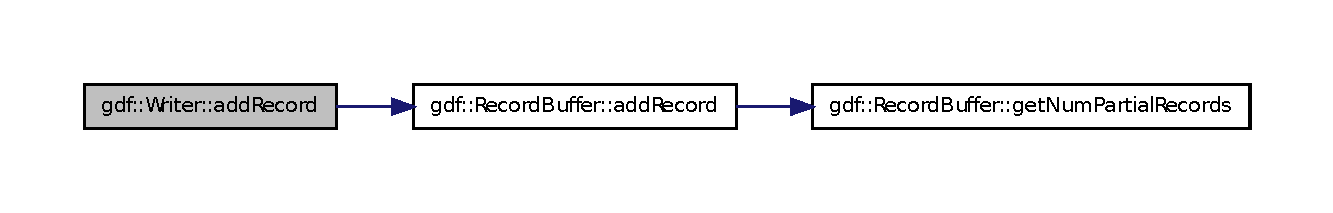
\includegraphics[width=400pt]{classgdf_1_1_writer_aa067a56c9699ad0c0a9fbebf83724dec_cgraph}
\end{center}
\end{figure}


\hypertarget{classgdf_1_1_writer_aeb0e491af4de91e79469634d8b3ecc5d}{
\index{gdf::Writer@{gdf::Writer}!addSamplePhys@{addSamplePhys}}
\index{addSamplePhys@{addSamplePhys}!gdf::Writer@{gdf::Writer}}
\subsubsection[{addSamplePhys}]{\setlength{\rightskip}{0pt plus 5cm}void gdf::Writer::addSamplePhys (
\begin{DoxyParamCaption}
\item[{const size\_\-t}]{ channel\_\-idx, }
\item[{const float64}]{ value}
\end{DoxyParamCaption}
)}}
\label{classgdf_1_1_writer_aeb0e491af4de91e79469634d8b3ecc5d}


Add sample in physical units to a channel. 

The sample value is converted from the channels \mbox{[}physmin,physmax\mbox{]} to the range of \mbox{[}digmin,digmax\mbox{]} and then cast to the correct data type. 
\begin{DoxyParams}{Parameters}
\item[\mbox{\tt[in]} {\em channel\_\-idx}]index of the channel written to \item[\mbox{\tt[in]} {\em value}]sample value in physical units \end{DoxyParams}


Here is the call graph for this function:
\nopagebreak
\begin{figure}[H]
\begin{center}
\leavevmode
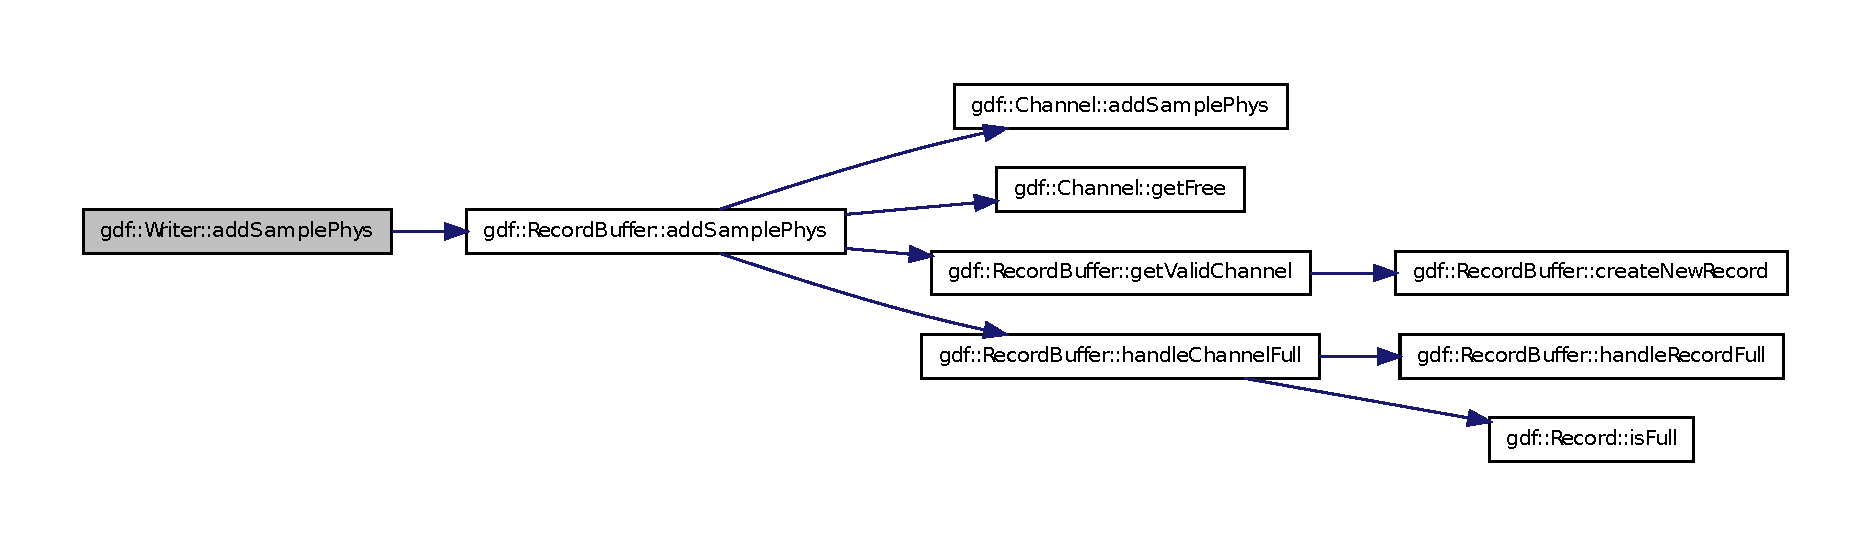
\includegraphics[width=400pt]{classgdf_1_1_writer_aeb0e491af4de91e79469634d8b3ecc5d_cgraph}
\end{center}
\end{figure}


\hypertarget{classgdf_1_1_writer_a072237c5d82136be71668611a27111fc}{
\index{gdf::Writer@{gdf::Writer}!addSampleRaw@{addSampleRaw}}
\index{addSampleRaw@{addSampleRaw}!gdf::Writer@{gdf::Writer}}
\subsubsection[{addSampleRaw}]{\setlength{\rightskip}{0pt plus 5cm}template$<$typename T $>$ void gdf::Writer::addSampleRaw (
\begin{DoxyParamCaption}
\item[{const size\_\-t}]{ channel\_\-idx, }
\item[{const T}]{ value}
\end{DoxyParamCaption}
)\hspace{0.3cm}{\ttfamily  \mbox{[}inline\mbox{]}}}}
\label{classgdf_1_1_writer_a072237c5d82136be71668611a27111fc}


Add a raw sample to channel. 

The sample value is cast to the correct data type, but no range checking is performed 
\begin{DoxyParams}{Parameters}
\item[\mbox{\tt[in]} {\em channel\_\-idx}]index of the channel written to \item[\mbox{\tt[in]} {\em value}]raw sample value in physical units \end{DoxyParams}


Here is the call graph for this function:
\nopagebreak
\begin{figure}[H]
\begin{center}
\leavevmode
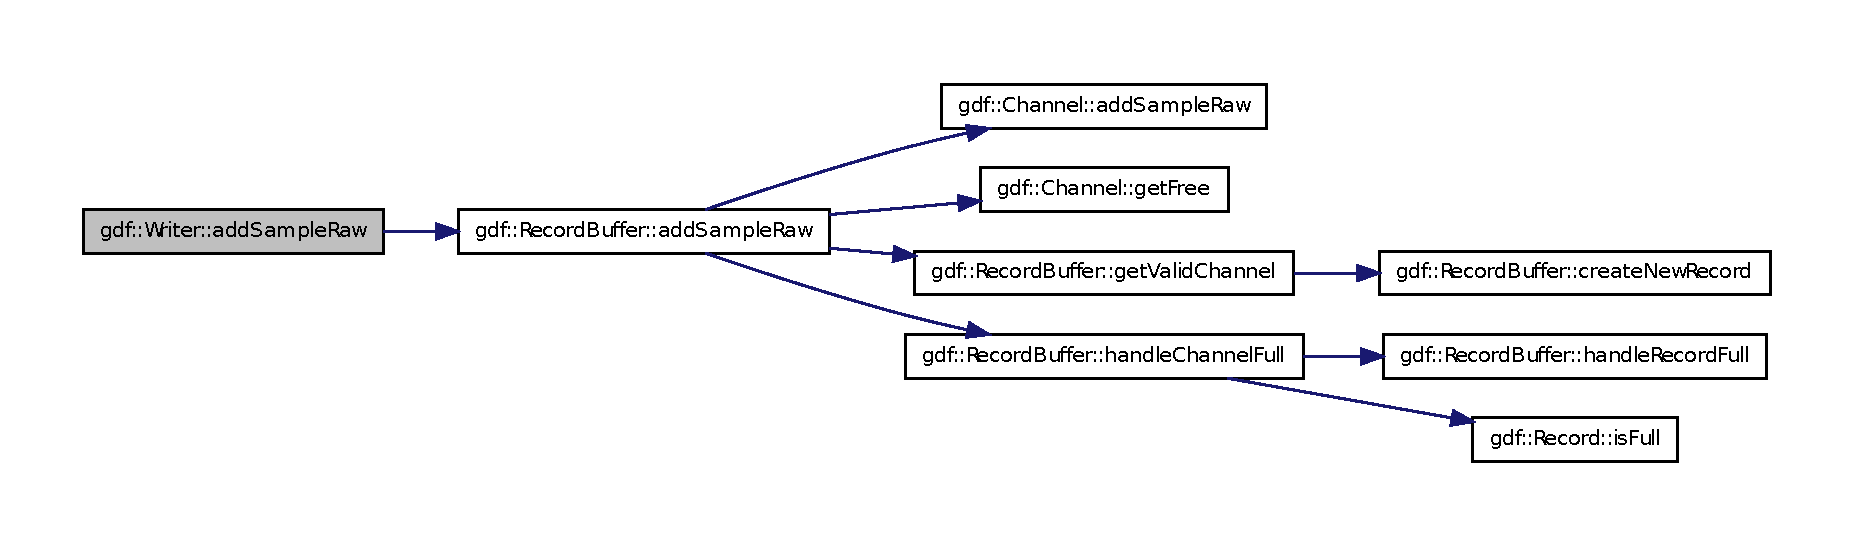
\includegraphics[width=400pt]{classgdf_1_1_writer_a072237c5d82136be71668611a27111fc_cgraph}
\end{center}
\end{figure}


\hypertarget{classgdf_1_1_writer_a78c344714054c13d96e0c85af24ad19f}{
\index{gdf::Writer@{gdf::Writer}!blitFromSerialBufferPhys@{blitFromSerialBufferPhys}}
\index{blitFromSerialBufferPhys@{blitFromSerialBufferPhys}!gdf::Writer@{gdf::Writer}}
\subsubsection[{blitFromSerialBufferPhys}]{\setlength{\rightskip}{0pt plus 5cm}void gdf::Writer::blitFromSerialBufferPhys (
\begin{DoxyParamCaption}
\item[{const double $\ast$}]{ buf, }
\item[{const std::vector$<$ size\_\-t $>$ \&}]{ samples\_\-per\_\-channel}
\end{DoxyParamCaption}
)}}
\label{classgdf_1_1_writer_a78c344714054c13d96e0c85af24ad19f}


Blit data from a serial buffer. 

Instead of streaming samples as they come, the complete data is provided in an array of type double. In the buffer channels have to be arranged sequentially. I.e. all samples from channel 1 are followed by all samles from channel 2, and so on. This function attempts to keep memory overhead low by filling record by record whenever possible. 
\begin{DoxyParams}{Parameters}
\item[\mbox{\tt[in]} {\em buf}]Buffer \item[\mbox{\tt[in]} {\em samples\_\-per\_\-channel}]A vector containing the number of samples in each channel. \end{DoxyParams}


Here is the call graph for this function:
\nopagebreak
\begin{figure}[H]
\begin{center}
\leavevmode
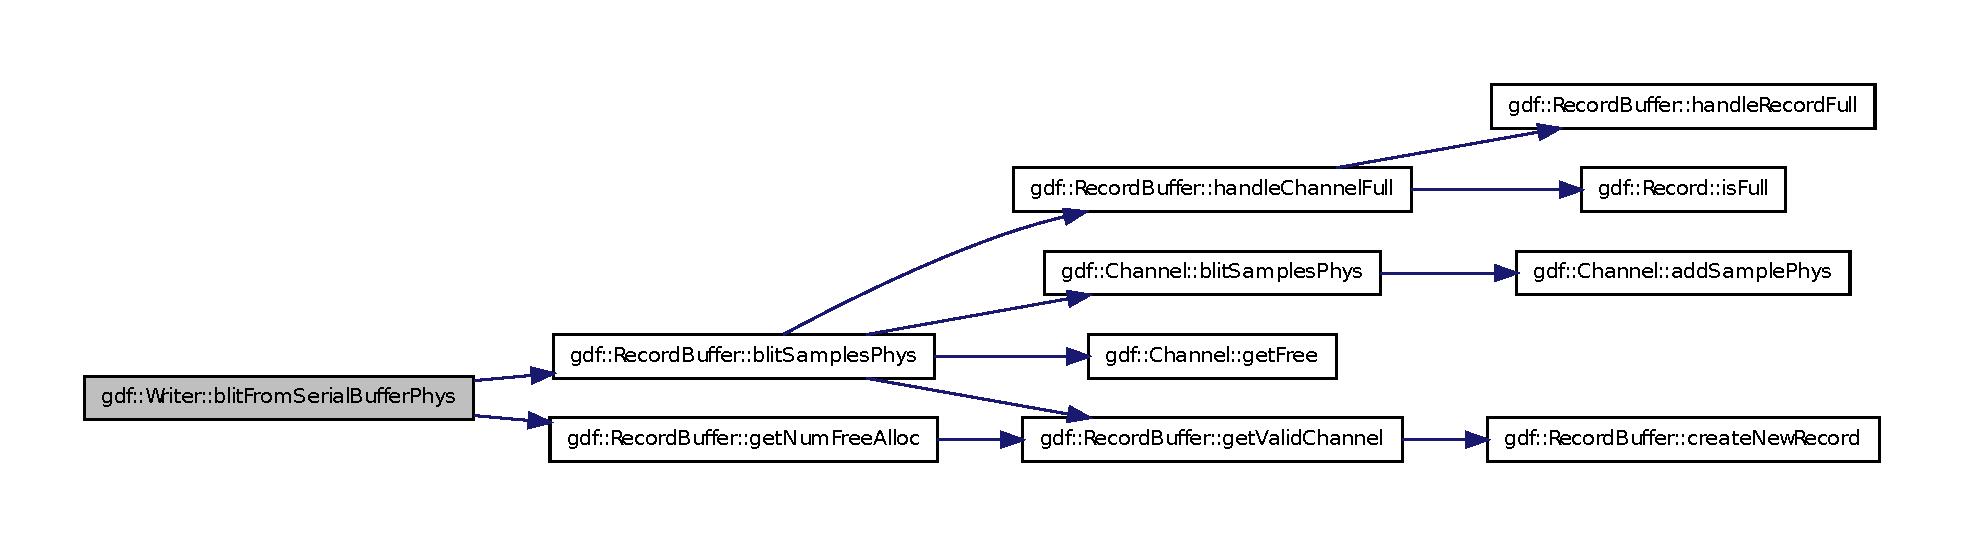
\includegraphics[width=400pt]{classgdf_1_1_writer_a78c344714054c13d96e0c85af24ad19f_cgraph}
\end{center}
\end{figure}


\hypertarget{classgdf_1_1_writer_a3e01dfba57c77e5cac1db767de79b650}{
\index{gdf::Writer@{gdf::Writer}!blitSamplesPhys@{blitSamplesPhys}}
\index{blitSamplesPhys@{blitSamplesPhys}!gdf::Writer@{gdf::Writer}}
\subsubsection[{blitSamplesPhys}]{\setlength{\rightskip}{0pt plus 5cm}void gdf::Writer::blitSamplesPhys (
\begin{DoxyParamCaption}
\item[{const size\_\-t}]{ channel\_\-idx, }
\item[{const float64 $\ast$}]{ values, }
\item[{size\_\-t}]{ num}
\end{DoxyParamCaption}
)}}
\label{classgdf_1_1_writer_a3e01dfba57c77e5cac1db767de79b650}


Blit a number of samples in physical units to channel. 

The sample values are converted from the channels \mbox{[}physmin,physmax\mbox{]} to the range of \mbox{[}digmin,digmax\mbox{]} and then cast to the correct data type. 
\begin{DoxyParams}{Parameters}
\item[\mbox{\tt[in]} {\em channel\_\-idx}]index of the channel written to \item[\mbox{\tt[in]} {\em values}]array of sample values in physical units \item[\mbox{\tt[in]} {\em num}]number of samples to blit \end{DoxyParams}


Here is the call graph for this function:
\nopagebreak
\begin{figure}[H]
\begin{center}
\leavevmode
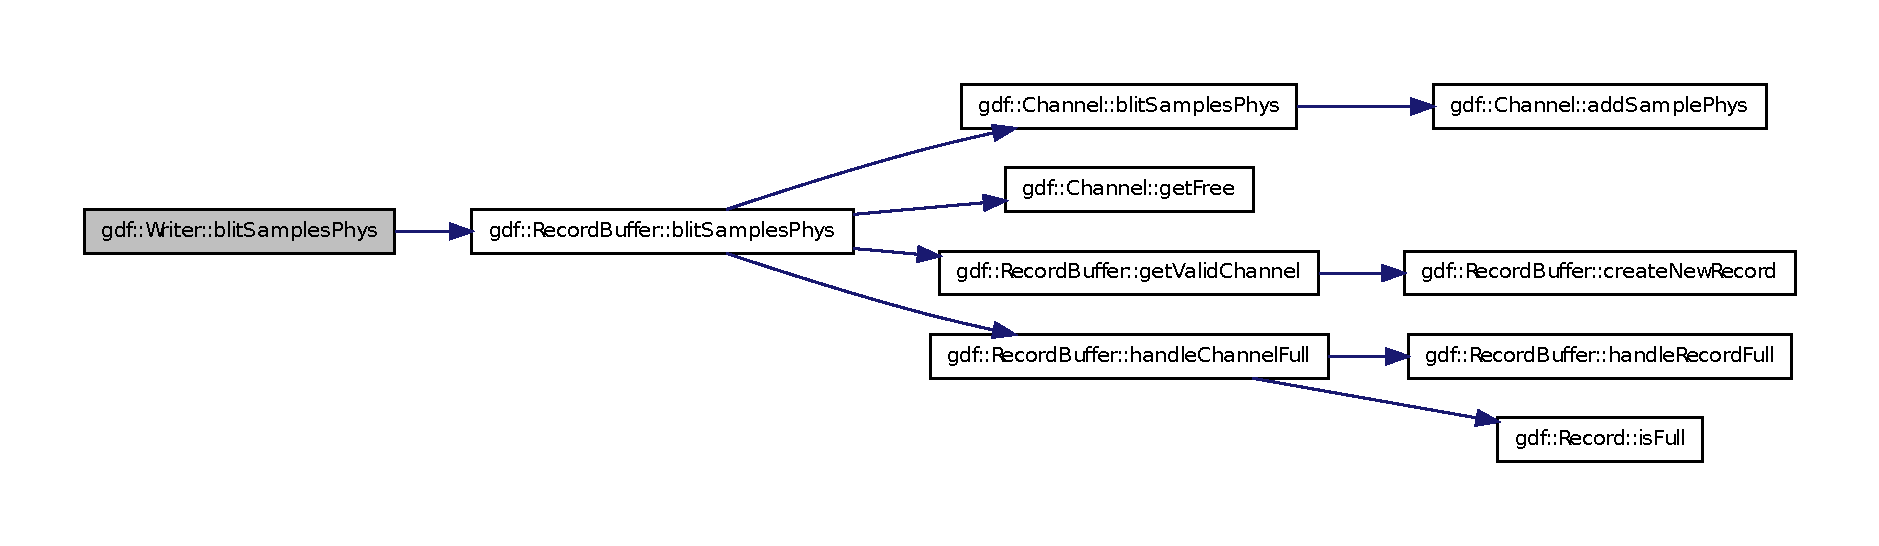
\includegraphics[width=400pt]{classgdf_1_1_writer_a3e01dfba57c77e5cac1db767de79b650_cgraph}
\end{center}
\end{figure}


\hypertarget{classgdf_1_1_writer_af8b7e224467b9b706e4eaec7672d8399}{
\index{gdf::Writer@{gdf::Writer}!blitSamplesPhys@{blitSamplesPhys}}
\index{blitSamplesPhys@{blitSamplesPhys}!gdf::Writer@{gdf::Writer}}
\subsubsection[{blitSamplesPhys}]{\setlength{\rightskip}{0pt plus 5cm}void gdf::Writer::blitSamplesPhys (
\begin{DoxyParamCaption}
\item[{const size\_\-t}]{ channel\_\-idx, }
\item[{const std::vector$<$ float64 $>$ \&}]{ values}
\end{DoxyParamCaption}
)}}
\label{classgdf_1_1_writer_af8b7e224467b9b706e4eaec7672d8399}


Blit a number of samples in physical units to channel. 

The sample values are converted from the channels \mbox{[}physmin,physmax\mbox{]} to the range of \mbox{[}digmin,digmax\mbox{]} and then cast to the correct data type. 
\begin{DoxyParams}{Parameters}
\item[\mbox{\tt[in]} {\em channel\_\-idx}]index of the channel written to \item[\mbox{\tt[in]} {\em values}]vector of sample values in physical units \end{DoxyParams}


Here is the call graph for this function:
\nopagebreak
\begin{figure}[H]
\begin{center}
\leavevmode
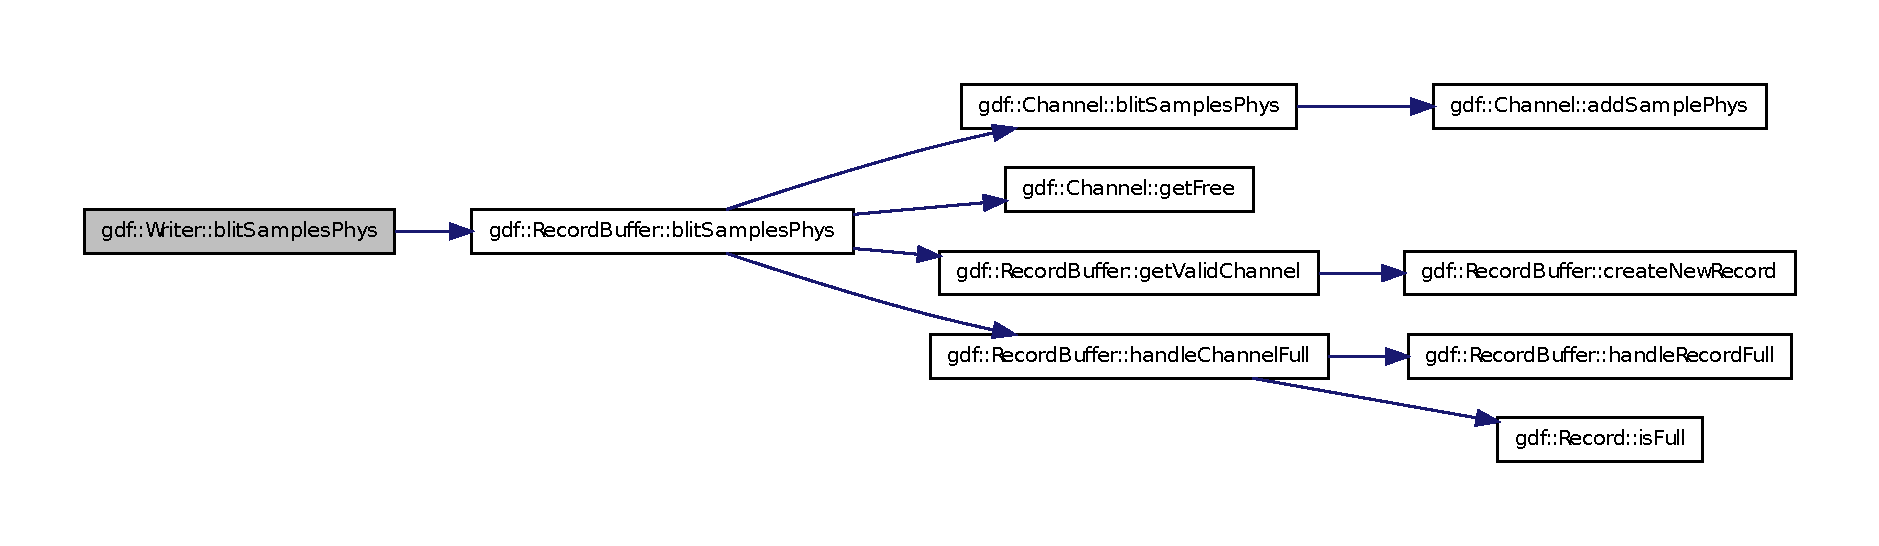
\includegraphics[width=400pt]{classgdf_1_1_writer_af8b7e224467b9b706e4eaec7672d8399_cgraph}
\end{center}
\end{figure}


\hypertarget{classgdf_1_1_writer_a2faf6a7c8aa18f81aadd0ff42eeb5caf}{
\index{gdf::Writer@{gdf::Writer}!blitSamplesRaw@{blitSamplesRaw}}
\index{blitSamplesRaw@{blitSamplesRaw}!gdf::Writer@{gdf::Writer}}
\subsubsection[{blitSamplesRaw}]{\setlength{\rightskip}{0pt plus 5cm}template$<$typename T $>$ void gdf::Writer::blitSamplesRaw (
\begin{DoxyParamCaption}
\item[{const size\_\-t}]{ channel\_\-idx, }
\item[{const T $\ast$}]{ values, }
\item[{size\_\-t}]{ num}
\end{DoxyParamCaption}
)\hspace{0.3cm}{\ttfamily  \mbox{[}inline\mbox{]}}}}
\label{classgdf_1_1_writer_a2faf6a7c8aa18f81aadd0ff42eeb5caf}


Blit a number of raw samples to channel. 

The sample values are cast to the correct data type, but no range checking is performed 
\begin{DoxyParams}{Parameters}
\item[\mbox{\tt[in]} {\em channel\_\-idx}]index of the channel written to \item[\mbox{\tt[in]} {\em values}]array of raw sample value \item[\mbox{\tt[in]} {\em num}]number of samples to blit \end{DoxyParams}


Here is the call graph for this function:
\nopagebreak
\begin{figure}[H]
\begin{center}
\leavevmode
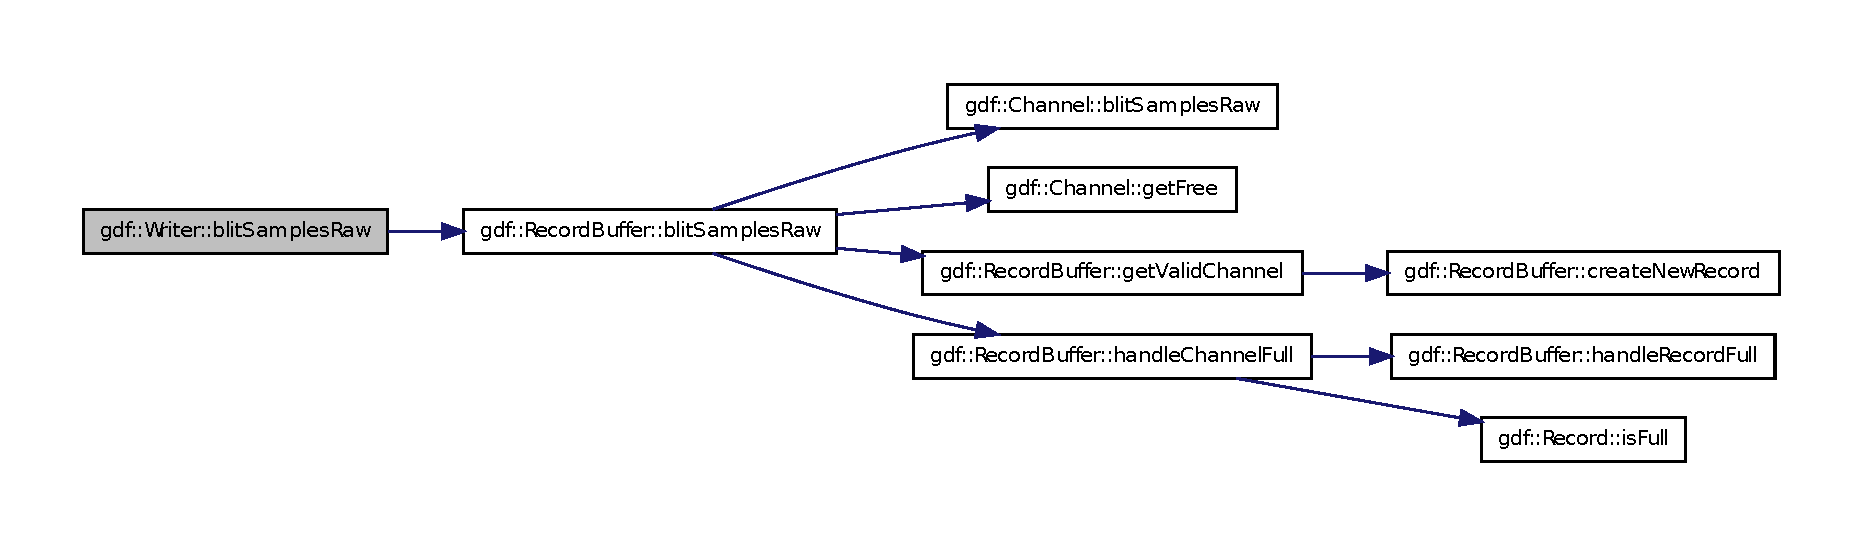
\includegraphics[width=400pt]{classgdf_1_1_writer_a2faf6a7c8aa18f81aadd0ff42eeb5caf_cgraph}
\end{center}
\end{figure}


\hypertarget{classgdf_1_1_writer_ae9eb09e9e7017fafaa6c367ec74d66bb}{
\index{gdf::Writer@{gdf::Writer}!blitSamplesRaw@{blitSamplesRaw}}
\index{blitSamplesRaw@{blitSamplesRaw}!gdf::Writer@{gdf::Writer}}
\subsubsection[{blitSamplesRaw}]{\setlength{\rightskip}{0pt plus 5cm}template$<$typename T $>$ void gdf::Writer::blitSamplesRaw (
\begin{DoxyParamCaption}
\item[{const size\_\-t}]{ channel\_\-idx, }
\item[{const std::vector$<$ T $>$ \&}]{ values}
\end{DoxyParamCaption}
)\hspace{0.3cm}{\ttfamily  \mbox{[}inline\mbox{]}}}}
\label{classgdf_1_1_writer_ae9eb09e9e7017fafaa6c367ec74d66bb}


Blit a number of raw samples to channel. 

The sample values are cast to the correct data type, but no range checking is performed 
\begin{DoxyParams}{Parameters}
\item[\mbox{\tt[in]} {\em channel\_\-idx}]index of the channel written to \item[\mbox{\tt[in]} {\em values}]vector of raw sample value \end{DoxyParams}


Here is the call graph for this function:
\nopagebreak
\begin{figure}[H]
\begin{center}
\leavevmode
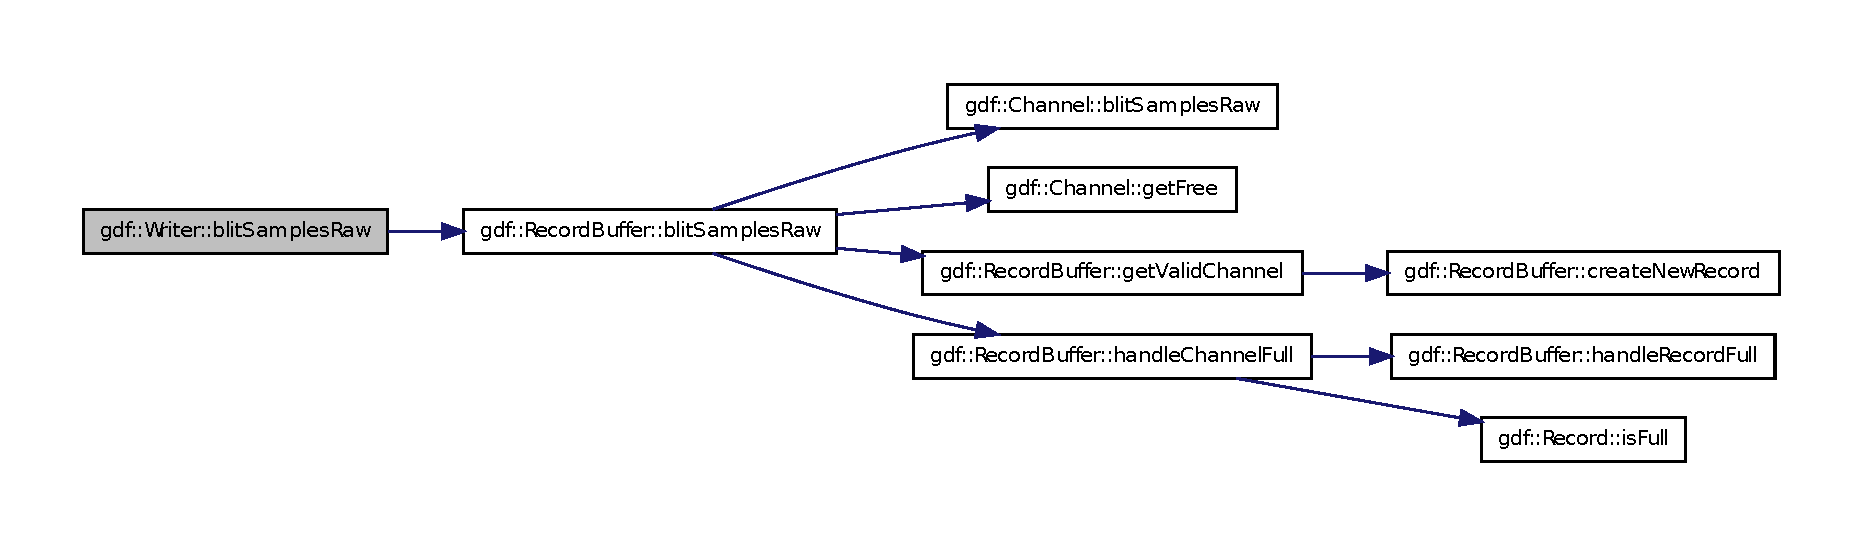
\includegraphics[width=400pt]{classgdf_1_1_writer_ae9eb09e9e7017fafaa6c367ec74d66bb_cgraph}
\end{center}
\end{figure}


\hypertarget{classgdf_1_1_writer_ae5856d4b6ca98e7af552d99d830433c9}{
\index{gdf::Writer@{gdf::Writer}!close@{close}}
\index{close@{close}!gdf::Writer@{gdf::Writer}}
\subsubsection[{close}]{\setlength{\rightskip}{0pt plus 5cm}void gdf::Writer::close (
\begin{DoxyParamCaption}
{}
\end{DoxyParamCaption}
)}}
\label{classgdf_1_1_writer_ae5856d4b6ca98e7af552d99d830433c9}


Close file. 

File is closed if open. Prior to closing, events are written to the file. 

Here is the call graph for this function:
\nopagebreak
\begin{figure}[H]
\begin{center}
\leavevmode
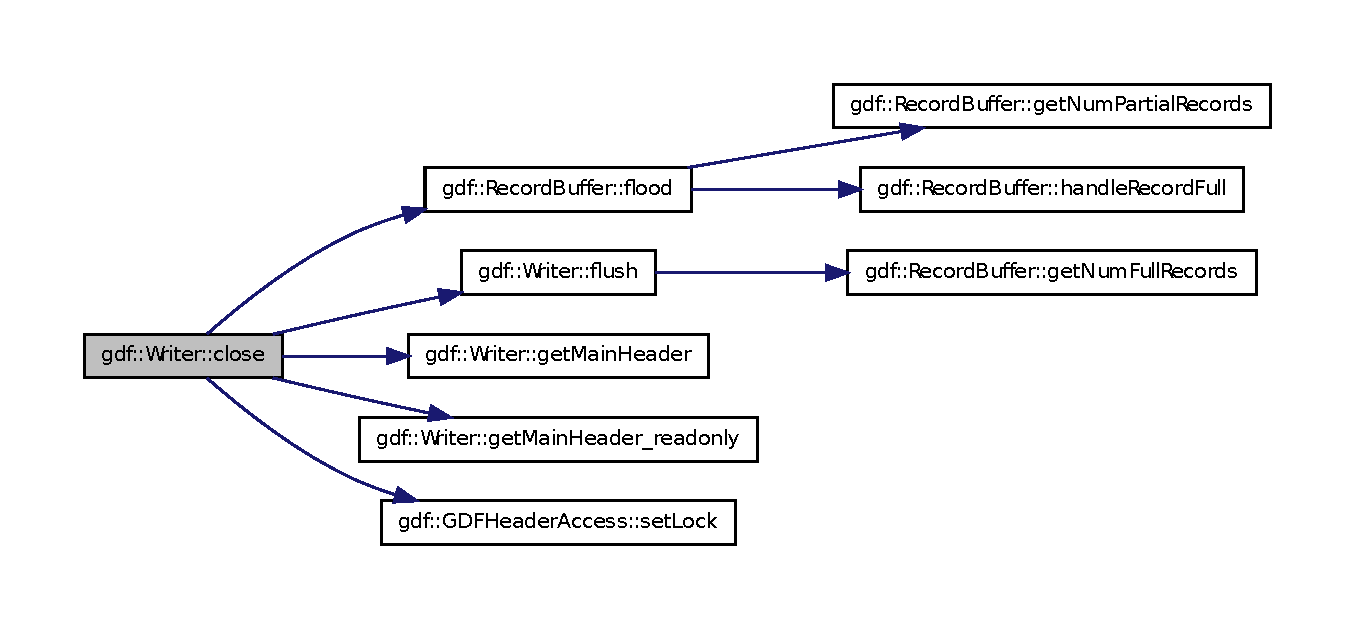
\includegraphics[width=400pt]{classgdf_1_1_writer_ae5856d4b6ca98e7af552d99d830433c9_cgraph}
\end{center}
\end{figure}




Here is the caller graph for this function:
\nopagebreak
\begin{figure}[H]
\begin{center}
\leavevmode
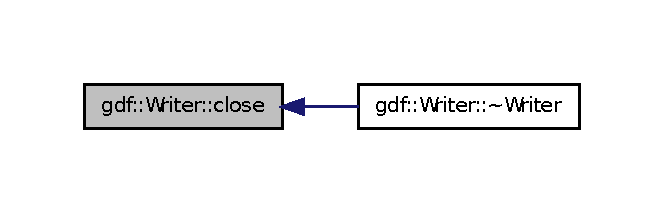
\includegraphics[width=318pt]{classgdf_1_1_writer_ae5856d4b6ca98e7af552d99d830433c9_icgraph}
\end{center}
\end{figure}


\hypertarget{classgdf_1_1_writer_ab0dc03f3e4f125695c40c09ce66d9d16}{
\index{gdf::Writer@{gdf::Writer}!createSignal@{createSignal}}
\index{createSignal@{createSignal}!gdf::Writer@{gdf::Writer}}
\subsubsection[{createSignal}]{\setlength{\rightskip}{0pt plus 5cm}bool gdf::Writer::createSignal (
\begin{DoxyParamCaption}
\item[{size\_\-t}]{ index, }
\item[{bool}]{ throwexc = {\ttfamily false}}
\end{DoxyParamCaption}
)}}
\label{classgdf_1_1_writer_ab0dc03f3e4f125695c40c09ce66d9d16}


Create a signal. 

Signals have to be created before they can be configured and stored. 
\begin{DoxyParams}{Parameters}
\item[\mbox{\tt[in]} {\em index}]index of the signal \item[\mbox{\tt[in]} {\em throwexc}]if true, \hyperlink{classgdf_1_1exception_1_1signal__exists}{exception::signal\_\-exists} may be thrown \end{DoxyParams}
\begin{DoxyReturn}{Returns}
true on success 
\end{DoxyReturn}
\hypertarget{classgdf_1_1_writer_a984bb670f2ca17c85916924877edab39}{
\index{gdf::Writer@{gdf::Writer}!open@{open}}
\index{open@{open}!gdf::Writer@{gdf::Writer}}
\subsubsection[{open}]{\setlength{\rightskip}{0pt plus 5cm}void gdf::Writer::open (
\begin{DoxyParamCaption}
\item[{const int}]{ flags = {\ttfamily writer\_\-ev\_\-file}}
\end{DoxyParamCaption}
)}}
\label{classgdf_1_1_writer_a984bb670f2ca17c85916924877edab39}


Opens file for writing and writes Header. 

Prior to opening the file, \hyperlink{classgdf_1_1_g_d_f_header_access_a16f91d1cb964f0acd3c842cf87c9d959}{GDFHeaderAccess::sanitize()} is called. Exceptions thrown by \hyperlink{classgdf_1_1_g_d_f_header_access_a16f91d1cb964f0acd3c842cf87c9d959}{GDFHeaderAccess::sanitize()} are checked if there are errors and/or warnings. In the presence of errors the exception is forwarded immediately, and in case of warnings the file is opened but the exception is still forwarded. If the file exists, it is not opened unless the file\_\-overwrite flag is set. 
\begin{DoxyParams}{Parameters}
\item[\mbox{\tt[in]} {\em flags}]Flags... \end{DoxyParams}

\begin{DoxyExceptions}{Exceptions}
\item[{\em \hyperlink{classgdf_1_1exception_1_1header__issues}{exception::header\_\-issues}}]\item[{\em \hyperlink{classgdf_1_1exception_1_1file__exists}{exception::file\_\-exists}}]\end{DoxyExceptions}


Here is the call graph for this function:
\nopagebreak
\begin{figure}[H]
\begin{center}
\leavevmode
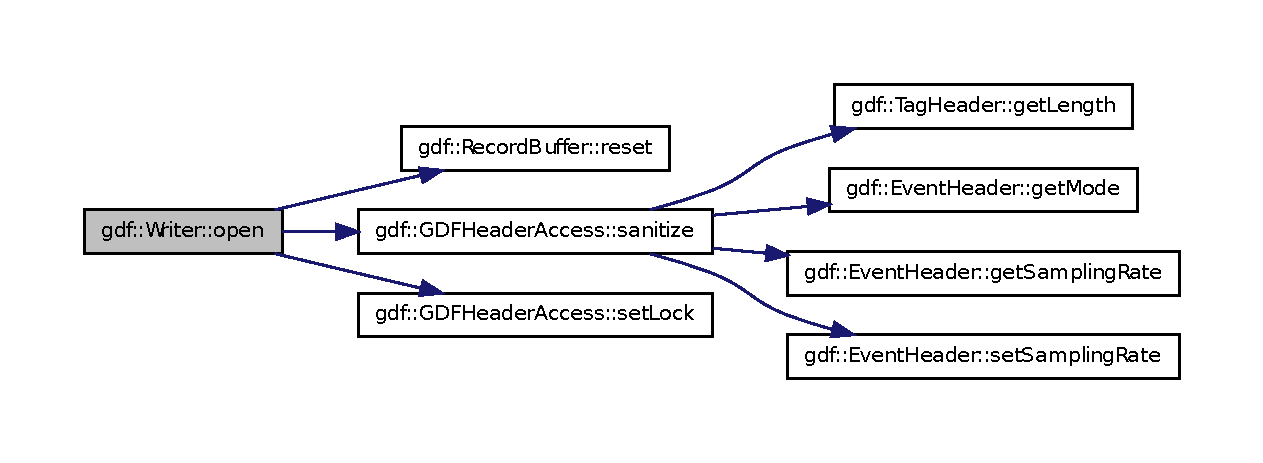
\includegraphics[width=400pt]{classgdf_1_1_writer_a984bb670f2ca17c85916924877edab39_cgraph}
\end{center}
\end{figure}




Here is the caller graph for this function:
\nopagebreak
\begin{figure}[H]
\begin{center}
\leavevmode
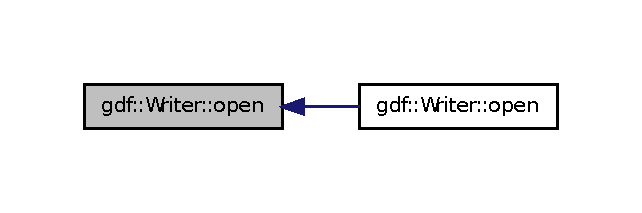
\includegraphics[width=308pt]{classgdf_1_1_writer_a984bb670f2ca17c85916924877edab39_icgraph}
\end{center}
\end{figure}


\hypertarget{classgdf_1_1_writer_ab493c0c6beb99d11d0cba1a229681e44}{
\index{gdf::Writer@{gdf::Writer}!open@{open}}
\index{open@{open}!gdf::Writer@{gdf::Writer}}
\subsubsection[{open}]{\setlength{\rightskip}{0pt plus 5cm}void gdf::Writer::open (
\begin{DoxyParamCaption}
\item[{const std::string}]{ filename, }
\item[{const int}]{ flags = {\ttfamily writer\_\-ev\_\-file}}
\end{DoxyParamCaption}
)}}
\label{classgdf_1_1_writer_ab493c0c6beb99d11d0cba1a229681e44}


Opens file for writing and writes Header. 

Convenience function. Calls setFilename prior to opening the file 
\begin{DoxyParams}{Parameters}
\item[\mbox{\tt[in]} {\em filename}]Full path name to the file. \item[\mbox{\tt[in]} {\em flags}]Flags... \end{DoxyParams}

\begin{DoxyExceptions}{Exceptions}
\item[{\em \hyperlink{classgdf_1_1exception_1_1header__issues}{exception::header\_\-issues}}]\item[{\em \hyperlink{classgdf_1_1exception_1_1file__exists}{exception::file\_\-exists}}]\end{DoxyExceptions}


Here is the call graph for this function:
\nopagebreak
\begin{figure}[H]
\begin{center}
\leavevmode
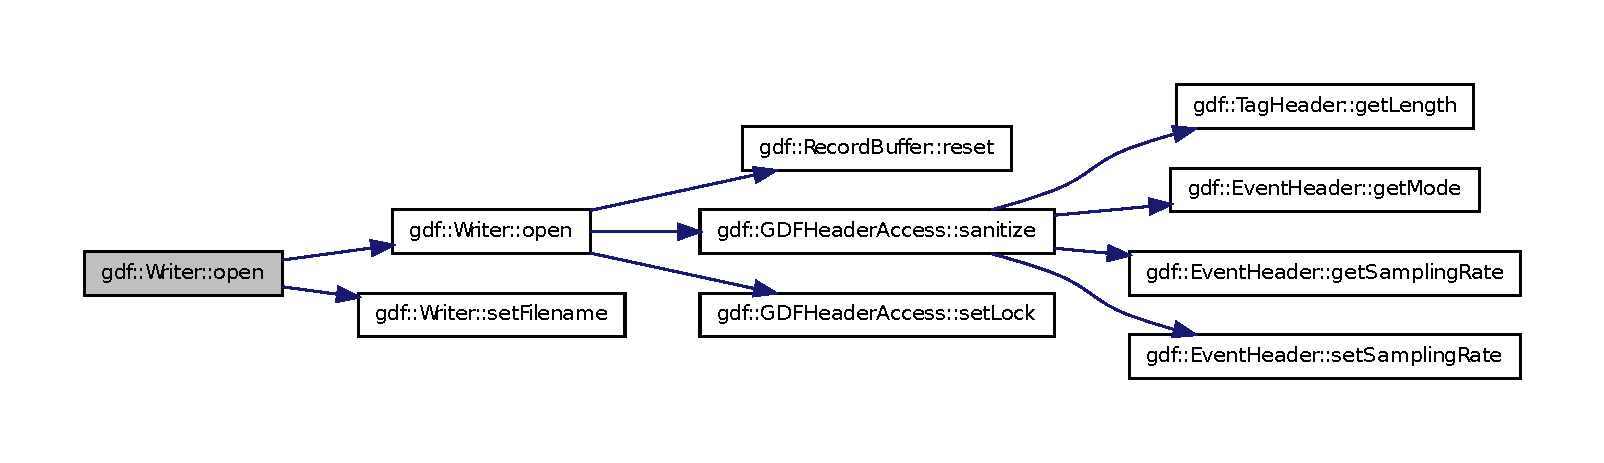
\includegraphics[width=400pt]{classgdf_1_1_writer_ab493c0c6beb99d11d0cba1a229681e44_cgraph}
\end{center}
\end{figure}


\hypertarget{classgdf_1_1_writer_ab69e32b0fb120731544cbff10d6e3a3f}{
\index{gdf::Writer@{gdf::Writer}!relocateSignal@{relocateSignal}}
\index{relocateSignal@{relocateSignal}!gdf::Writer@{gdf::Writer}}
\subsubsection[{relocateSignal}]{\setlength{\rightskip}{0pt plus 5cm}void gdf::Writer::relocateSignal (
\begin{DoxyParamCaption}
\item[{size\_\-t}]{ src, }
\item[{size\_\-t}]{ dst}
\end{DoxyParamCaption}
)}}
\label{classgdf_1_1_writer_ab69e32b0fb120731544cbff10d6e3a3f}


Change signal index. 

The new index must not exist 
\begin{DoxyParams}{Parameters}
\item[\mbox{\tt[in]} {\em src}]old index of first signal \item[\mbox{\tt[in]} {\em dst}]new index of second signal \end{DoxyParams}
\hypertarget{classgdf_1_1_writer_ac8b0924c5b5721d01274e73c02b0d69f}{
\index{gdf::Writer@{gdf::Writer}!setEventMode@{setEventMode}}
\index{setEventMode@{setEventMode}!gdf::Writer@{gdf::Writer}}
\subsubsection[{setEventMode}]{\setlength{\rightskip}{0pt plus 5cm}void gdf::Writer::setEventMode (
\begin{DoxyParamCaption}
\item[{uint8}]{ mode}
\end{DoxyParamCaption}
)}}
\label{classgdf_1_1_writer_ac8b0924c5b5721d01274e73c02b0d69f}


Set Event Mode. 

mode can be 1 or 3 1: (default) Events are stored as position,type pairs 3: Events are stored with position and type, associated to a channel and have a duration or value. 
\begin{DoxyParams}{Parameters}
\item[\mbox{\tt[in]} {\em mode}]event mode \end{DoxyParams}


Here is the call graph for this function:
\nopagebreak
\begin{figure}[H]
\begin{center}
\leavevmode
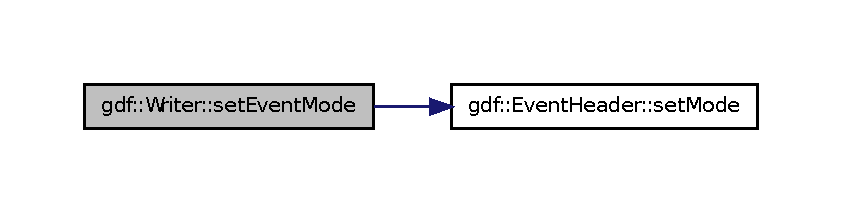
\includegraphics[width=400pt]{classgdf_1_1_writer_ac8b0924c5b5721d01274e73c02b0d69f_cgraph}
\end{center}
\end{figure}


\hypertarget{classgdf_1_1_writer_aeabb4626bd62684d0c9e5d3222e83fff}{
\index{gdf::Writer@{gdf::Writer}!setEventSamplingRate@{setEventSamplingRate}}
\index{setEventSamplingRate@{setEventSamplingRate}!gdf::Writer@{gdf::Writer}}
\subsubsection[{setEventSamplingRate}]{\setlength{\rightskip}{0pt plus 5cm}void gdf::Writer::setEventSamplingRate (
\begin{DoxyParamCaption}
\item[{float32}]{ fs = {\ttfamily -\/1}}
\end{DoxyParamCaption}
)}}
\label{classgdf_1_1_writer_aeabb4626bd62684d0c9e5d3222e83fff}


Set Sampling Rate associated with event positions. 

Events are not actually sampled, but their position is stored in samples rather than seconds. In order to convert event positions between time and sample, this sampling rate is used. If Sampling rate is not set (or set to $<$= 0 ), fs is set to the highest signal sampling rate. 
\begin{DoxyParams}{Parameters}
\item[\mbox{\tt[in]} {\em fs}]sampling rate \end{DoxyParams}


Here is the call graph for this function:
\nopagebreak
\begin{figure}[H]
\begin{center}
\leavevmode
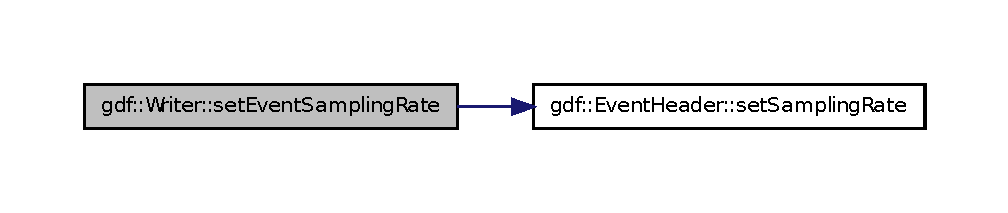
\includegraphics[width=400pt]{classgdf_1_1_writer_aeabb4626bd62684d0c9e5d3222e83fff_cgraph}
\end{center}
\end{figure}


\hypertarget{classgdf_1_1_writer_ad8cab49e3b866304802924707fd9d367}{
\index{gdf::Writer@{gdf::Writer}!setFilename@{setFilename}}
\index{setFilename@{setFilename}!gdf::Writer@{gdf::Writer}}
\subsubsection[{setFilename}]{\setlength{\rightskip}{0pt plus 5cm}void gdf::Writer::setFilename (
\begin{DoxyParamCaption}
\item[{std::string}]{ filename}
\end{DoxyParamCaption}
)}}
\label{classgdf_1_1_writer_ad8cab49e3b866304802924707fd9d367}


set filename for later opening 


\begin{DoxyParams}{Parameters}
\item[\mbox{\tt[in]} {\em filename}]Full path name to the file \end{DoxyParams}


Here is the caller graph for this function:
\nopagebreak
\begin{figure}[H]
\begin{center}
\leavevmode
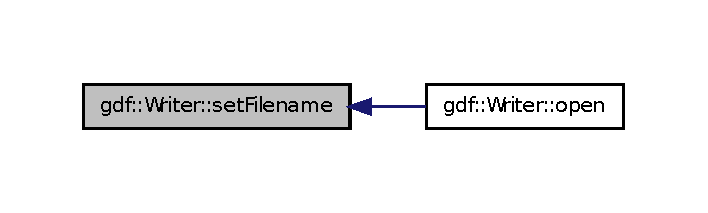
\includegraphics[width=340pt]{classgdf_1_1_writer_ad8cab49e3b866304802924707fd9d367_icgraph}
\end{center}
\end{figure}


\hypertarget{classgdf_1_1_writer_a15b2d4702b41521a1dba4fe8b7f2986a}{
\index{gdf::Writer@{gdf::Writer}!setMaxFullRecords@{setMaxFullRecords}}
\index{setMaxFullRecords@{setMaxFullRecords}!gdf::Writer@{gdf::Writer}}
\subsubsection[{setMaxFullRecords}]{\setlength{\rightskip}{0pt plus 5cm}void gdf::Writer::setMaxFullRecords (
\begin{DoxyParamCaption}
\item[{size\_\-t}]{ num}
\end{DoxyParamCaption}
)}}
\label{classgdf_1_1_writer_a15b2d4702b41521a1dba4fe8b7f2986a}


Set number of full records that are kept in memory before the buffer is flushed. 


\begin{DoxyParams}{Parameters}
\item[\mbox{\tt[in]} {\em num}]number of records \end{DoxyParams}


Here is the caller graph for this function:
\nopagebreak
\begin{figure}[H]
\begin{center}
\leavevmode
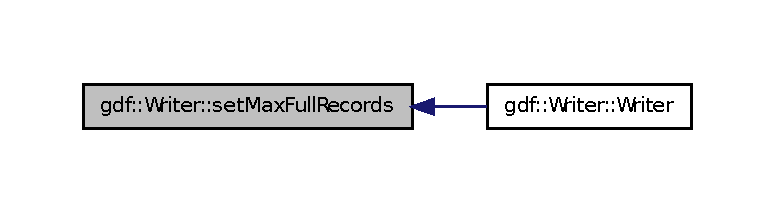
\includegraphics[width=372pt]{classgdf_1_1_writer_a15b2d4702b41521a1dba4fe8b7f2986a_icgraph}
\end{center}
\end{figure}


\hypertarget{classgdf_1_1_writer_a25563ed9d61e7b6935dc09bc469c9eb7}{
\index{gdf::Writer@{gdf::Writer}!swapSignals@{swapSignals}}
\index{swapSignals@{swapSignals}!gdf::Writer@{gdf::Writer}}
\subsubsection[{swapSignals}]{\setlength{\rightskip}{0pt plus 5cm}void gdf::Writer::swapSignals (
\begin{DoxyParamCaption}
\item[{size\_\-t}]{ a, }
\item[{size\_\-t}]{ b}
\end{DoxyParamCaption}
)}}
\label{classgdf_1_1_writer_a25563ed9d61e7b6935dc09bc469c9eb7}


Swap to signals. 

Both signals must exist. 
\begin{DoxyParams}{Parameters}
\item[\mbox{\tt[in]} {\em a}]index of first signal \item[\mbox{\tt[in]} {\em b}]index of second signal \end{DoxyParams}


The documentation for this class was generated from the following files:\begin{DoxyCompactItemize}
\item 
include/GDF/Writer.h\item 
src/Writer.cpp\end{DoxyCompactItemize}

\hypertarget{classgdf_1_1exception_1_1wrong__eventmode}{
\section{gdf::exception::wrong\_\-eventmode Class Reference}
\label{classgdf_1_1exception_1_1wrong__eventmode}\index{gdf::exception::wrong\_\-eventmode@{gdf::exception::wrong\_\-eventmode}}
}


Operation on wrong event mode.  




{\ttfamily \#include $<$Exceptions.h$>$}

\subsection*{Public Member Functions}
\begin{DoxyCompactItemize}
\item 
\hypertarget{classgdf_1_1exception_1_1wrong__eventmode_a552a358aa767076ebebf94604d70029b}{
{\bfseries wrong\_\-eventmode} (std::string str)}
\label{classgdf_1_1exception_1_1wrong__eventmode_a552a358aa767076ebebf94604d70029b}

\end{DoxyCompactItemize}


\subsection{Detailed Description}
Operation on wrong event mode. 

The documentation for this class was generated from the following file:\begin{DoxyCompactItemize}
\item 
include/GDF/Exceptions.h\end{DoxyCompactItemize}

\printindex
\end{document}
